\documentclass[twocolumn,10pt]{article}
\pdfoutput=1 % This must be in the first 5 lines to tell arXiv to use pdfLaTeX
\usepackage[l2tabu,orthodox]{nag}
\usepackage[utf8x]{inputenc}
\usepackage[british]{babel}
\usepackage{microtype}
\usepackage{amsmath}
\usepackage[all]{onlyamsmath}
\usepackage{newtxtext}
\usepackage{newtxmath}
\usepackage[caption=false]{subfig}
\usepackage{booktabs}
\usepackage{upquote}
\usepackage{graphicx}
\usepackage{url}
\usepackage{algorithm}
\usepackage{algpseudocode}
\usepackage{color}
\usepackage[cm]{fullpage}
\usepackage{multirow}
\usepackage{authblk}

\frenchspacing
\uchyph=0

\newlength{\figureWidthOneColumn}
\setlength{\figureWidthOneColumn}{0.4\textwidth}

\newlength{\figureWidthTwoColumn}
\setlength{\figureWidthTwoColumn}{0.8\textwidth}

\newcommand{\todo}[1]{\textbf{\textcolor{red}{To do: #1}}}
\newcommand{\pb}[1]{\vspace{0.75ex}\noindent{\textbf{#1}}}
\newcommand{\liwc}[1]{\textsc{#1}}
\newcommand{\word}[1]{\textit{`#1'}}

%==================================================================================================
\begin{document}

\title{An Empirical Analysis of the Internet Engineering Task Force with Computational Methods}

\author[1]{Mladen Karan}
\author[1]{Prashant Khare}
\author[2]{Ravi Shekhar}
\author[1]{Matthew Russell Barnes}
\author[1]{Waleed Iqbal}
\author[3]{Junaid Qadir}
\author[4]{Stephen McQuistin}
\author[1]{Richard G. Clegg}
\author[1]{Patrick Healey}
\author[5]{Matthew Purver}
\author[1]{Ignacio Castro}
\author[6]{Gareth Tyson}
\author[7]{Colin Perkins}

\affil[1]{Queen Mary University of London}
\affil[2]{University of Essex}
\affil[3]{Qatar University}
\affil[4]{University of St Andrews}
\affil[5]{Jo\v{z}ef Stefan Institute}
\affil[6]{Hong Kong University of Science \& Technology}
\affil[7]{University of Glasgow}

\date{7 October 2024}

\maketitle
%==================================================================================================
\begin{abstract}
  % Four sentences:
  %  - State the problem
  %  - Say why it's an interesting problem
  %  - Say what your solution achieves
  %  - Say what follows from your solution

  The Internet requires interoperability between networks, systems, and
  applications, as well as cooperation among a growing number of
  stakeholders. The Internet Engineering Task Force (IETF) is critical in
  supporting this cooperation and interoperability by bringing together
  interested parties and standardising the protocols that power the
  Internet, such as IP or HTTP. Our work covers more 20 years of IETF
  data, and analyses the participants of the IETF, the emails they
  exchange, and the documents they produce. We show how these data can be
  used to understand who are these Internet actors, and their interests as
  well as how Internet's growth and maturity has given rise to a longer and
  complex standardisation process where participants gain and exercise
  influence and how this is reflected in the language they use and the
  interactions they have.
  
\end{abstract}
%==================================================================================================
\section{Introduction}

% Paragraph 1: Motivation. At a high level, what is the problem area you
% are working in and why is it important? It is important to set the larger
% context here. Why is the problem of interest and importance to the larger
% community?

Network protocol standards are crucial for successful operation of the
Internet.  A successful standard provides a basis for interoperability
between systems developed by competing vendors, and supports the growth of
an open ecosystem of products and services. Further, the process by which
network protocol standards are developed, comprising multiple rounds of
open feedback and review, has proven remarkably effective in designing
high-quality and robust protocols, many of which see widespread deployment
and use. Understanding the Internet standards development process, and how
it produces successful protocols is, therefore, important if we are to
understand the Internet and how it has evolved.

One of the main organisations that develops protocol standards is the
Internet Engineering Task Force (IETF). The IETF was founded in 1986,
following on from the US Government-funded effort that developed the early
Internet. It has since grown to become a global community of network
protocol designers, vendors, network operators, and researchers that
develop and publish open network protocol standards and operational
guidelines.  The IETF publishes its standards, and other documents, in
the RFC series.\footnote{\url{https://www.rfc-editor.org}} This series
comprises around 9,000 documents, authored over more than 50 years,
and provides a rich history of the development of the Internet and
its protocols \cite{RFC8700}.


% Paragraph 2: What is the specific problem considered in this paper? This
% paragraph narrows down the topic area of the paper. In the first
% paragraph you have established general context and importance. Here you
% establish specific context and background.

Standardisation is an inherently social and political process
\cite{RFC2026,RFC7282}, requiring cooperation and consensus among a growing
number of stakeholders.

It is important to gain a coherent understanding of the activities that
take place within the IETF, as well as the key factors that may predict
the success of a protocol standard.


% Paragraph 3: "In this paper, we show that...". This is the key paragraph
% in the introduction - you summarize, in one paragraph, what are the main
% contributions of your paper, given the context established in paragraphs
% 1 and 2. What's the general approach taken? Why are the specific results
% significant? The story is not what you did, but rather:
%  - what you show, new ideas, new insights
%  - why interesting, important?
% State your contributions: these drive the entire paper.  Contributions
% should be refutable claims, not vague generic statements.

In this paper, we ...

% Paragraph 4: What are the differences between your work, and what others
% have done? Keep this at a high level, as you can refer to future sections
% where specific details and differences will be given, but it is important
% for the reader to know what is new about this work compared to other work
% in the area.


This paper summarises and expands on our prior work
\cite{mcquistin:2021:characterising,khare:2022:web-we-weave,
healey:2023:power,mcquistin:2023:errare,khare:2023:tracing,
karan:2023:leda,healey:2023:power-frontiers,barnes:2024:temporal}.

% Paragraph 5: "We structure the remainder of this paper as follows." Give
% the reader a road-map for the rest of the paper. Try to avoid redundant
% phrasing, "In Section 2, In section 3, ..., In Section 4, ... ", etc.

We structure the remainder of this paper as follows.
Section \ref{sec:background} introduces the IETF and the Internet Standards
development process, and reviews the data with which we work.
Section \ref{sec:trends-documents} considers trends in document production,
complexity, and correctness.
Section \ref{sec:trends-demographics} moves on to consider the people who
are involved in Internet standards development and how the demographics of
the community have shifted over time.
Section \ref{sec:org-dyn} studies the interaction between participants,
explores who has influence and impact in the IETF and how that influence
is evident in their activities, and the dynamics of communications within
the IETF.
Section \ref{sec:language} considers communications within the IETF from
the perspective of language to explore whether there are differences in
linguistic patterns and language use in more influential participants,
and to consider how the use of language reflects the consensus-driven
nature of the standards development process.
Section \ref{sec:success-factors} then considers factors that lead to
success, exploring what makes a document likely to be published as an
RFC and what makes a successful participant.
Finally, we review related work in Section \ref{sec:related} and conclude
in Section \ref{sec:conclusions}.

%==================================================================================================
\section{Background and Datasets}
\label{sec:background}

% The following is from our IMC 2021 paper:

We start by presenting an overview of the IETF, and the publication process
for RFCs, before outlining the data sources we use within this paper. We
also highlight the ethical considerations of accessing and processing this
data.


%--------------------------------------------------------------------------------------------------
\subsection{An IETF Primer}
\label{sec:background:ietf}

% The following is from our IMC 2021 paper:

%..................................................................................................
\pb{The IETF} is an open standards organisation, which develops
Internet standards via contributions and collaborations across a number of
voluntary stakeholders, including academics, consultants, industry
representatives, governments, and civil society organisations.  Through
extensive collaboration across contributors, the IETF, and associated
organisations, develops Internet standards and other documents. These are
published by the RFC Editor (\url{https://www.rfc-editor.org}) in four
\emph{publication streams}: the IETF stream, the Internet Research Task
Force (IRTF) stream, the Internet Architecture Board (IAB) stream, and the
Independent Submission stream.

There is also a fifth, legacy stream, comprising RFCs published prior to
the adoption of separate publication streams in July 2007 \cite{RFC4844}.
While the IETF is an open standards forum that develops technical standards
and operational guidelines for the Internet, the IRTF is an associated
organisation that promotes longer-term research, and the IAB provides
long-range technical direction for Internet development. The Independent
Submission stream ``allows RFC publication for some documents that are
outside the official IETF/IAB/IRTF process but are relevant to the Internet
community'' (\url{https://www.rfc-editor.org/about/independent}).

%..................................................................................................
\pb{The standards development process} is an inherently collaborative
activity.  Most day-to-day work is conducted on public mailing lists, in
conjunction with three plenary meetings and numerous interim working group
meetings per year. 
The mailing lists are broadly split into three categories: announcement
lists, where replies are not allowed; non-working group lists, for
discussing topics that do not relate to the work within an IETF working
group or IRTF research group; and working group and area lists, where
technical discussions take place.

The process of RFC publication begins with the submission of an
\emph{Internet-Draft}. Whereas anyone can post a draft, not all drafts
become RFCs. After a draft is first posted, multiple revisions might take
place resulting in multiple versions of the draft. Each new draft is
announced on one or more mailing lists related to the topic of the draft,
soliciting feedback and encouraging discussion. Drafts are initially posted
by individuals. For publication under the IETF stream, drafts must then be
adopted by a working group, where, via further revision, the draft may
ultimately be published as an RFC. The process of managing drafts, and the
degree and type of peer review conducted prior to their submission to the
RFC Editor for publication, differs between streams.

Once the technical development of the draft is complete its publication is
managed by the RFC Editor, who maintains the master archive of the RFC
documents, along with an index of metadata pertaining to the RFCs and their
authors. Finally, once an RFC has been published, deployment is voluntary,
and therefore not all RFCs are widely implemented.

%--------------------------------------------------------------------------------------------------
\subsection{Data Sources}
\label{sec:background:data}

% The following is adapted from our IMC 2021 paper and our IFIP TMA 2023
% paper, Section II:

We rely on a number of data sources to conduct our study.

%..................................................................................................
\pb{IETF Datatracker:}
The Datatracker\footnote{\url{https://datatracker.ietf.org/}} is the main
administrative database used by the IETF, IRTF, and IAB to coordinate their
work. It contains information about contributors, working groups,
documents, and meetings. The Datatracker provides comprehensive metadata
about authors, and the evolution of drafts as they work their way through
the standardisation process. The Datatracker was introduced in the early
2000s and its functionality has gradually been extended over time. It
contains limited historical data about RFCs produced before its creation,
but the IETF has back-filled some data from other records.  We have
extracted relevant metadata from the Datatracker, using its programmatic
REST API, for all RFCs published since 2001. This gives us data pertaining
to 4,512 authors, as well as richer metadata for 5,707 RFCs.

%..................................................................................................
\pb{RFC Editor:}
The RFC Editor maintains an index of all RFC publications, alongside
metadata related to each document, including its standardisation status,
publication stream, authors, and errata. We gather all entries for RFCs
published through the end of 2020, giving a total of 8,711 RFCs.

RFCs are not changed after publication, but the RFC Editor maintains a
public database of reported errata. The errata filing are separated into
\emph{technical errata}, mistakes in the technical content of the RFC that
are likely to result in incorrect, non-conforming, implementations of the
standards, and \emph{editorial errata} including spelling and punctuation
errors that do not otherwise impact the technical content.
Errata filed against RFCs published on the IETF stream are checked for
correctness by the RFC authors, working group chairs, and area directors.
IRTF errata are checked by the authors and the Internet Research Steering
Group. The IAB and Independent Submissions Editor check errata for their
streams. We collected\footnote{RFC errata are available at
\url{https://www.rfc-editor.org/errata.php}. We thank the RFC Editor for
making the underlying database available to us in machine-readable form for
this analysis.} the 6,759 errata reports submitted from January 2001 to the
end of December 2022 for analysis.

%..................................................................................................
\pb{Email archives and entity resolution:}
The IETF maintains reasonably complete email archives relating to working
group discussions, meeting, and other activities.\footnote{\url{https://mailarchive.ietf.org/}
with public IMAP access also available.} We gather all available messages
contained within this archive, covering 2,439,240 messages, sent from
74,646 unique email addresses, across 1,153 lists. This snapshot was taken
on April 18th 2021.

A key challenge is attributing each email to an individual contributor.
Although each, naturally, contains a \texttt{From:} header, we find that some
contributors use multiple addresses. Beyond this, it is necessary to map
each email to the respective person in the Datatracker and RFC Editor
datasets.  Thus, we perform entity resolution on email senders, and match
email senders with their Datatracker profiles. We assign each sender a
unique identifier, which is associated with a set of name and address
variations from the Datatracker. 

Entity resolution takes place in multiple stages.  First, we check if the
sender's email address has a Datatracker profile. If so, we associate all
of their Datatracker metadata with that person's unique identifier, and
label the message as having been sent by that identifier.  Next, if an
email's sender does not appear in the Datatracker, we check, based on their
name, if they have already been assigned a Datatracker record. If so, the
message is labelled as having been sent by that identifier, and the set of
names and addresses associated with that identifier is updated to include
the email's sender name and address.

These two stages -- matching with the Datatracker, and merging previously
seen names and addresses -- accounts for the majority (60\%) of messages.
If an email's sender is not in the Datatracker, and the name and address
has not been previously seen, a new person identifier is generated. This
accounts for a small portion (~10\%) of messages. This is reasonable, given
that Datatracker profiles have become necessary for many of the IETF's
day-to-day activities.

As a final processing step, we label each identifier as either representing
a \emph{contributor}, a \emph{role-based} address, or an \emph{automated}
sender. A contributor refers to any standard user participating in the
IETF; role-based identifiers reflect addresses that are used by the holders
of a particular organisational role, such as the IETF chair; and automated
identifiers are those addresses that are system-specific, such as GitHub or
IETF notification and announcement addresses. Role-based and automated
identifiers account for the remaining 30\% of messages.

Note, within the mail archive, spam-indicating headers are present for most
messages since 2009, and we confirm pre-filtering is performed by the IETF
mail servers.  As an extra validation step, we ran a spam filter over all
the archived messages and discarded those marked as spam. Both sources
indicate there is very little spam (less than 1\%), so it should not have
significant impact on our findings.

% \pb{Manually labelled dataset:} 
% We also use data collated by Nikkhah et al.~\cite{nikkhah2017statistical}.
% This dataset labels the ``success'', alongside other features like scope
% and value, of 251 RFCs.  155 of these also appear in our set of RFCs that
% have Datatracker metadata available. We later use this to explore the
% features that best predict the success of an RFC.

% \pb{Microsoft Academic citation data:}
% We use the Microsoft Academic Knowledge API to identify indexed academic
% work that cites each RFC. We use the Microsoft Academic Graph instead of
% other sources (\eg Google Scholar) as it provides time-stamped citations.

%..................................................................................................
\pb{Reproducibility and data access:}
We have developed a library, \texttt{ietfdata}, that fetches the RFC
Index, communicates with the IETF Datatracker API, and retrieves messages
from the IETF IMAP mail archives. This library appropriately regulates
access, caches data to minimise the impact on the infrastructure, and
performs necessary post-processing. This library is available as open
source and Ongoing development is coordinated on GitHub.%
\footnote{\url{https://github.com/glasgow-ipl/ietfdata}}


%--------------------------------------------------------------------------------------------------
\subsection{Ethical Considerations}
\label{sec:ethics}

% The following is adapted from our IMC 2021 paper:

The data we analyse is extracted from public IETF archives and APIs.  We
have taken steps to ensure ethical compliance.  To ensure that our access
to these services does not cause operational problems for the IETF, we are
in regular contact with the IETF Tools Team and Secretariat, as well as the
operators of the Datatracker and mailing list archive.  We have
discussed our work with IETF leadership (IETF and IAB Chairs, the IETF
Executive Director, and the IRTF Chair, who is a co-author on this paper)
and the RFC Editor to ensure that our access falls within their acceptable
use policies.

Participants in the IETF must agree to abide by the policies and procedures
described at \url{https://www.ietf.org/about/note-well}, including the privacy
policy at \url{https://www.ietf.org/privacy-statement}. These make explicit
provision that mailing list archives and the metadata contained in the
Datatracker system will be made public, and it is this public data that
we process to extract the aggregate statistics presented in Sections
\ref{sec:trends-documents}, \ref{sec:trends-demographics}, \ref{sec:org-dyn},
\ref{sec:language} as well as the features analysed in Section
\ref{sec:success-factors}. We transfer and store data securely, and retain
it only for the time needed to perform the analysis.  Since we operate
entirely using the public APIs provided by IETF, we have no access to
private data about individuals.

In balancing these ethical considerations with the reproducibility of our
work, we provide the tools needed to access the datasets from the relevant
IETF sources, rather than the data itself.


%==================================================================================================
\section{Trends in RFC Publication}
\label{sec:trends-documents}

% \begin{figure}
%   \centering
%   \includegraphics{figures/rfcs-by-year-stream.pdf}
%   \caption{Number of RFCs published per year}
%   \label{fig:rfcs-by-year}
% \end{figure}

To begin, we review trends in IETF standards publication. We consider the
rate of publication of documents in the RFC series, factors affecting the
publication rate, and the occurrence of errata reports, and answer the
following research questions:
\begin{enumerate}
  \item What factors affect the publication rate of RFCs and is the IETF
    standards development process getting faster or slower over time?
    (\S\ref{sec:trends-documents:production})

  \item Are the standards produced by the IETF broadly correct? Do the
    reported errata indicate problems with the standards development
    process in general, or in particular areas, and is the IETF getting
    better or worse at producing correct RFCs over time?
    (\S\ref{sec:trends-documents:errata})

\end{enumerate}

%--------------------------------------------------------------------------------------------------
\subsection{RFC Production and Complexity}
\label{sec:trends-documents:production}

RFC production trends show clear evidence that the IETF is a mature
standards development organisation. The peak of activity was in the 1990s
and early 2000s, with the initial broad deployment of the Internet, and the
organisation has since entered more of a development and maintenance mode
of operation. There are clear signs that the complexity of the installed
base of protocols is slowing development of new technologies.

% The following is from our IMC 2021 paper, Section 3.1:

%..................................................................................................
\pb{RFC Publication Rate:}
In total, 8,711 RFCs have been published through to the end of 2020.
Figure~\ref{fig:rfcs_by_area} shows how publication trends, in terms of
IETF areas and non-IETF streams, have changed over time. We identify three
broad publication phases in the RFC series. First, in 1969 through 1974,
RFCs are published at a rapid rate during the initial development of the
ARPANET. Then, from 1975 through 1985, development slows. This reflects a
relatively small community that is gaining real-world experience with the
network and developing a small core of applications and protocols. Finally,
with the creation of the IETF and the introduction of the National Science
Foundation Network (NSFNET) in 1986, both the community, and the number of
RFCs published, starts to expand rapidly. This is further driven by the
opening of the network to commercial and public use in the mid-1990s.
The annual RFC publication rate was highest in 2005, at the peak
of the standardisation efforts for SIP and related standards for voice-over-IP
and Internet telephony. The rate of publication has slowed in recent years,
following the completion of large work programmes relating to HTTP/2 and
WebRTC.

\begin{figure}
  \centering
  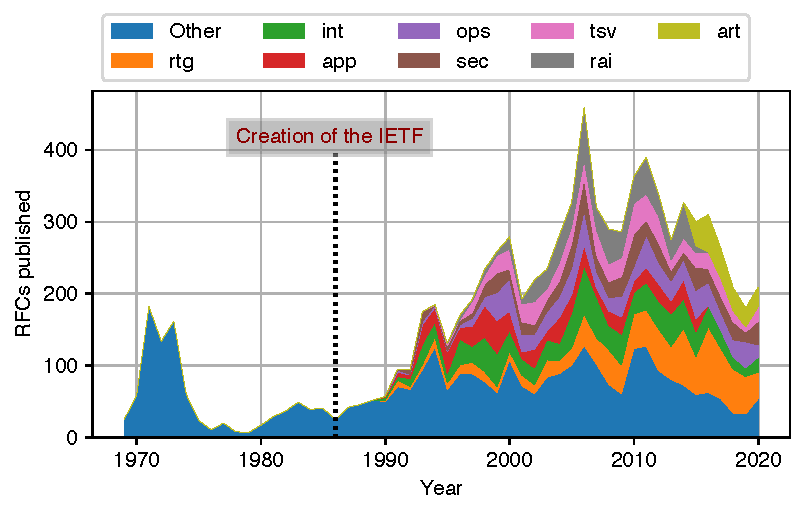
\includegraphics[width=\figureWidthOneColumn]{figures-prev/imc-2021/documents/rfcs_areas.pdf}
  \caption{
    Number of RFCs published over time, subdivided by IETF Area.
    The areas are 
    \emph{art} -- applications and real-time;
    \emph{app} -- applications;
    \emph{int} -- internetworking;
    \emph{ops} -- operations and management;
    \emph{rai} -- real-time applications and infrastructure;
    \emph{rtg} -- routing;
    \emph{sec} -- security; and
    \emph{tsv} -- transport and services.
    The \emph{other} category includes legacy RFCs, pre-dating the creation
    of the IETF, and RFCs published in non-IETF publication streams such as
    the IRTF, IAB, and the Independent stream.
  }
  \label{fig:rfcs_by_area}
\end{figure}

%..................................................................................................
\pb{Role of Working Groups:}
From the creation of the IETF in 1986 the growing community, with its
interests in an increasing set of applications and protocols, has been
split into a number of \emph{working groups}.\footnote{There are 122
active working groups at the time of writing, organised into 7 areas.
The number of groups varies over time, but is typically in the range
100-150.} These working groups are each chartered with a well-defined
programme of work and exist within \emph{areas} that have a broader focus.  

As shown in Figure~\ref{fig:rfcs_by_area}, the output of
different areas has remained relatively stable over time. The most notable
trends begin with the creation of the Real-time Applications and
Infrastructure (rai) area from within the Transport (tsv) area, and its
later merger with the Applications (app) area to become the Applications
and Real-Time (art) area around 2014. Additionally, we also observe the
significant growth in output of the Routing (rtg) area, owing to the
ongoing development of standards for MPLS, service function chaining, and
fat tree routing in data centres.

To give a sense for the broader productivity of the IETF,
Figure~\ref{fig:pub_wgs_yearly} shows the number of working groups that
publish RFCs each year. This highlights how the structure of the IETF has
grown to accommodate its larger community: in the early 1990s, fewer than
20 working groups were published an RFC each year, while in recent years
there has typically been at least 60 working group publishing RFCs, with
a peak of 97 working groups publishing RFCs in 2011 (the number of groups
publishing RFCs is less than the total number of groups, because it takes
time for the work of a new group to reach maturity).

\begin{figure}
  \centering
  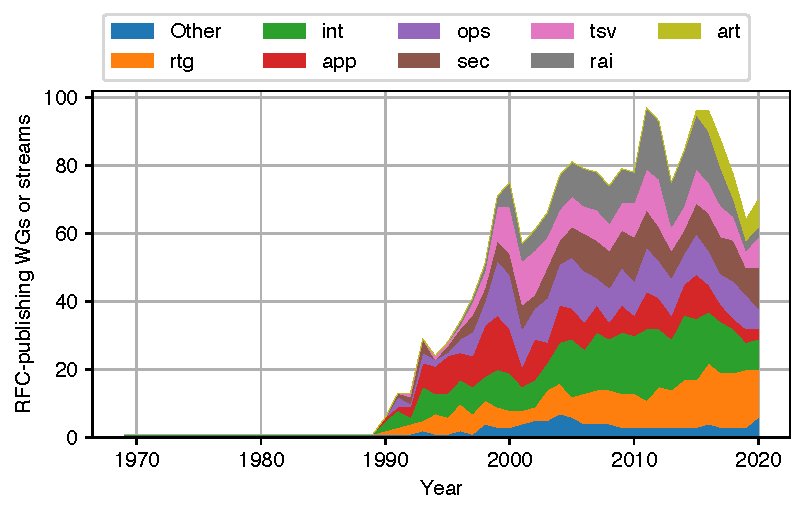
\includegraphics[width=\figureWidthOneColumn]{figures-prev/imc-2021/documents/unique_wgs_per_year_areas.pdf}
  \caption{
    Number of groups publishing RFCs over time, subdivided by IETF Area.
    The areas are as described in Figure~\ref{fig:rfcs_by_area}.
  }
  \label{fig:pub_wgs_yearly}
\end{figure}

%..................................................................................................
\pb{Internet-Drafts:}
Figure \ref{fig:drafts-by-date} shows the number of working documents,
known as Internet-drafts, that were active in the IETF over time. An
Internet-draft is a limited lifetime working document that expires after
six months, when replaced by a new version, or then published as an RFC.

We observe that the number of active drafts correlates more strongly with
the number of active working groups (Figure \ref{fig:pub_wgs_yearly}) than
with RFC publication (Figure \ref{fig:rfcs_by_area}).  This is largely to
be expected: an Internet-Draft is a work-in-progress document that is
proposed for adoption by, and discussion in, an IETF working group prior to
eventual publication as an RFC.  Competing proposals are often submitted as
drafts, to allow a working group to review them and make a decision how to
proceed, and hence not all drafts become RFCs. As we discuss in
\S\ref{sec:success-factors:documents}, draft adoption is a significant
milestone.

\begin{figure}
  \centering
  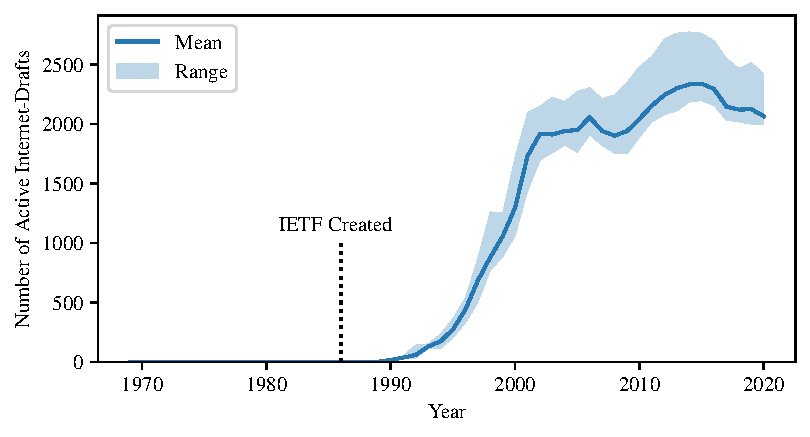
\includegraphics[width=\figureWidthOneColumn]{figures/drafts-by-date.pdf}
  \caption{
    Number of active drafts over time. Internet-Drafts, working documents
    of the IETF for work that was intended for eventual publication as an
    RFC, were introduction at the 13th IETF meeting in 1989.
  }
  \label{fig:drafts-by-date}
\end{figure}

%..................................................................................................
\pb{Factors Affecting Publication Rate:} 
The standards development process is taking longer.
Figure~\ref{fig:rfcs_days_to_pub} plots the median number of days from the
submission of the first draft of a document through to its publication as
an RFC. This shows a clear trend: RFCs are taking longer to make their way
through the standardisation and publication process. The median number of
days to publication was 469 in 2001, rising to 1,170 in 2020. 

\begin{figure}
  \centering
  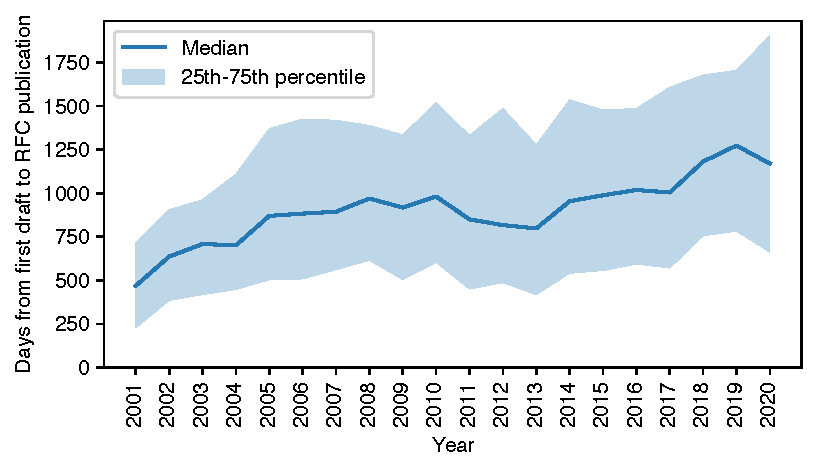
\includegraphics[width=\figureWidthOneColumn]{figures-prev/imc-2021/documents/day_counts_yearly.pdf}
  \caption{
    Days from first draft to RFC publication
  }
  \label{fig:rfcs_days_to_pub}
\end{figure}

Similarly, Figure~\ref{fig:drafts_year} shows the median number of
revisions each document undergoes before being published as an RFC. Days to
publication and number of revisions are strongly correlated, suggesting
that the time is spent making changes to the document. This may go some way
towards explaining the decline in output of the IETF: each RFC is taking
longer to produce, with more revisions before publication. 

\begin{figure}
  \centering
  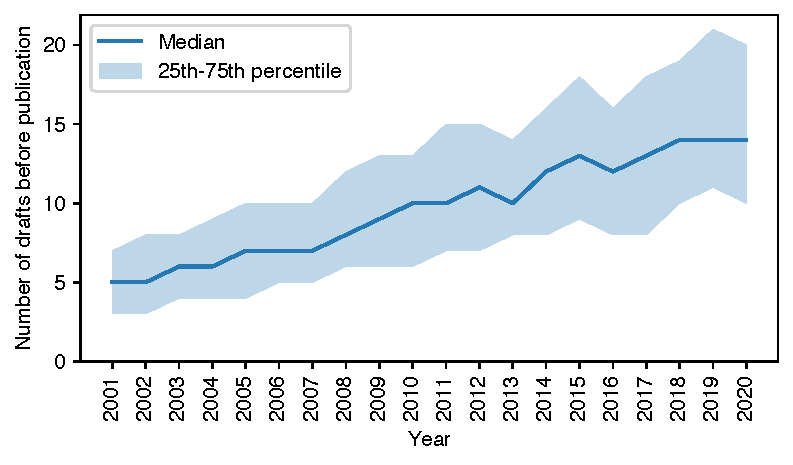
\includegraphics[width=\figureWidthOneColumn]{figures-prev/imc-2021/documents/draft_counts_yearly.pdf}
  \caption{
    Number of drafts per RFC
  }
  \label{fig:drafts_year}
\end{figure}


What factors affect the publication rate?  One may conjecture that this
slowdown is driven by longer RFCs that contain more material. Yet from the
median page count of RFCs, shown in Figure~\ref{fig:pages_year}, no clear
trend being visible. The increase in the duration of the standardisation
process for RFCs cannot be attributed to RFCs becoming longer: page counts
have remained stable. 

\begin{figure}
  \centering
  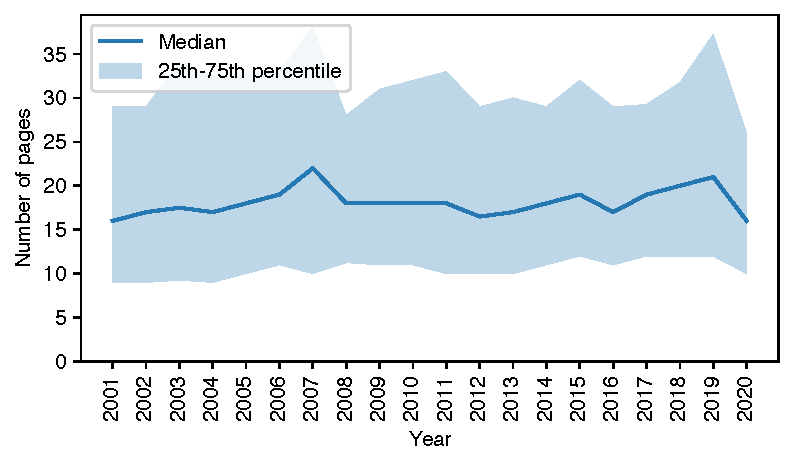
\includegraphics[width=\figureWidthOneColumn]{figures-prev/imc-2021/documents/page_counts_yearly_dt.pdf}
  \caption{
    RFC page counts
  }
  \label{fig:pages_year}
\end{figure}

The publication rate might also be slowing because RFCs are becoming more
complex. This could occur, for example, as a result of having to maintain
compatibility with older RFCs as the Internet has evolved and matured.
Figure~\ref{fig:updates_year} shows that this is the case, plotting the
proportion of RFCs that are published each year that update (i.e., extend
or augment) or obsolete (i.e., replace) one or more previously published
RFCs.  This percentage has slowly increased as the IETF has matured: in
2020, more than 30\% of RFCs updated or made obsolete a previous RFC.
%
Figure~\ref{fig:citations_year} expands on this, showing the median number
of citations from each RFC to other Internet-Drafts and RFCs. This
similarly shows that RFCs are increasingly referring to prior work.

\begin{figure}
  \centering
  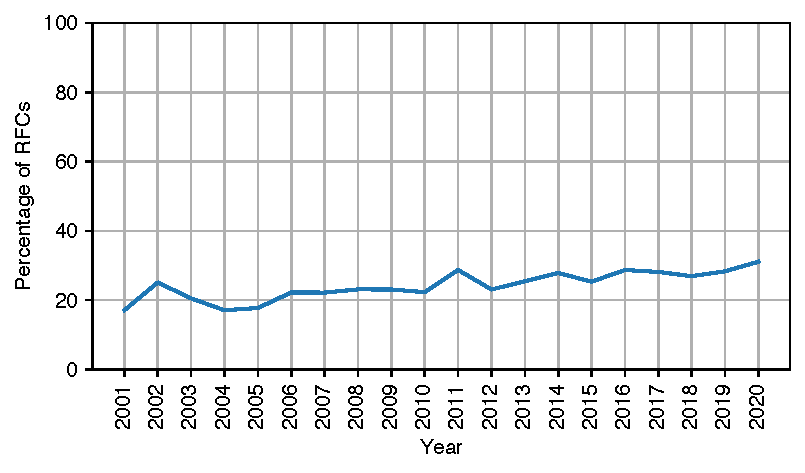
\includegraphics[width=\figureWidthOneColumn]{figures-prev/imc-2021/documents/update_obsolete_yearly_pct.pdf}
  \caption{
    RFCs that update or obsolete previous RFCs
  }
  \label{fig:updates_year}
\end{figure}

\begin{figure}
  \centering
  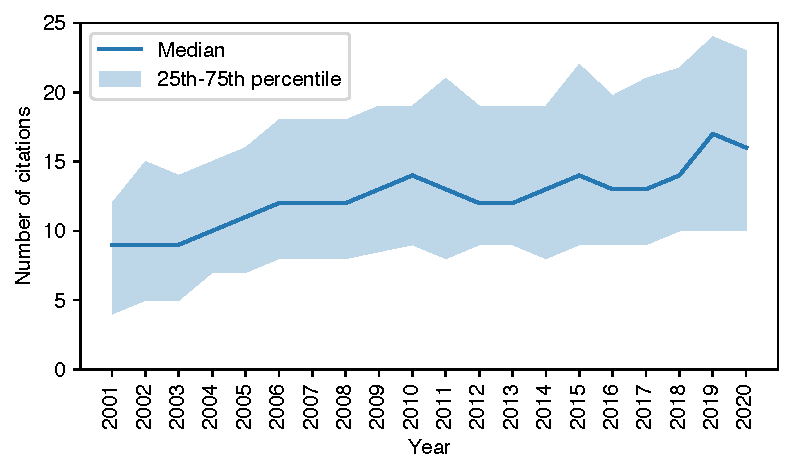
\includegraphics[width=\figureWidthOneColumn]{figures-prev/imc-2021/documents/cite_counts_yearly.pdf}
  \caption{
    Number of citations to other Internet-Drafts and RFCs per RFC in each
    year.
  }
  \label{fig:citations_year}
\end{figure}

Figure~\ref{fig:keyword_usage_rates} further confirms the growing complexity
of RFCs, showing how the use of normative language keywords has evolved
over time.  Keywords are used in RFCs to indicate the normative requirements
an RFC imposes on implementations. Figure~\ref{fig:keyword_usage_rates}
shows the total number of occurrences of each of the RFC 2119~\cite{RFC2119}
keywords (i.e., MUST, MUST NOT, REQUIRED, SHALL, SHALL NOT, SHOULD, SHOULD
NOT, RECOMMENDED, MAY, OPTIONAL), divided by the page count of the RFC. As
shown, the median number of keywords per page grew from 2001 through to
2010, indicating a growing number of requirements being expressed in RFCs,
before plateauing in recent years.

\begin{figure}
  \centering
  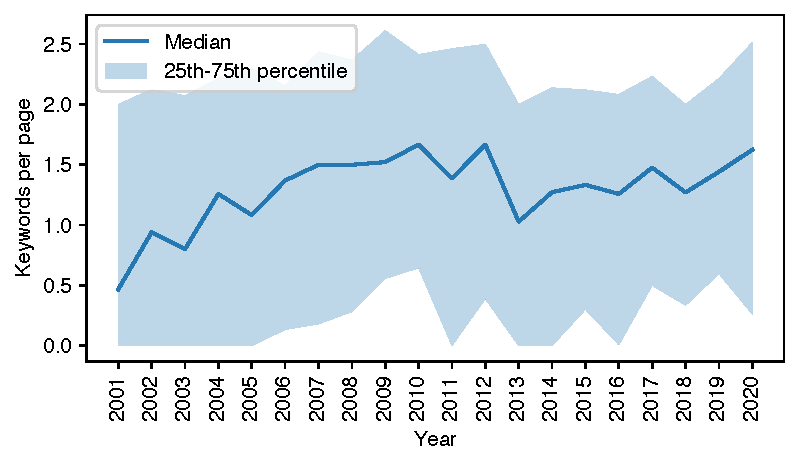
\includegraphics[width=\figureWidthOneColumn]{figures-prev/imc-2021/documents/keyword_usage_rate.pdf}
  \caption{
    Number of occurrences of normative language keywords per page in RFCs
    in each year.
  }
  \label{fig:keyword_usage_rates}
\end{figure}

%..................................................................................................
\pb{Summary:}
RFCs are taking longer to produce, and they go through a greater number
of revisions before publication. Further, they increasingly update or
reference previously published RFCs, and make greater use of
requirements-setting keywords. These are all hallmarks of a maturing
standards development organisation that must increasingly consider
compatibility with the installed based in the development of its standards.


%--------------------------------------------------------------------------------------------------
\subsection{RFC Errata}
\label{sec:trends-documents:errata}

% The following is from our TMA 2023 paper, Section I:

Mistakes can and do occur in published RFCs.  These errors can be reported
to the RFC Editor, and the RFC Editor makes the reports publicly available
and coordinates with the IETF, and the other publication streams, on their
verification. These errata can clarify editorial concerns as well as correct
substantive technical errors. Since the presence of significant errors in
its specification can undermine the success of a protocol, studying the
nature of these errata and their subsequent fixes is important.

In the following, we analyse the 6,759 errata filed with the RFC Editor
between 2001–2022, inclusive, documenting 3,288 editorial issues and 3,471
technical issues, and covering 2,240 RFCs, to understand the frequency
and causes of problems in RFCs.

% The following is from our TMA 2023 paper, Section III:

%..................................................................................................
\pb{Errata over Time:}
Figure~\ref{fig:errata_per_year} presents the number of errata filed, on
average per RFC, since 1969 based on the year of RFC publication.  The peak
in the number of errata per RFC occurs in 1981. Only 29 RFCs were published
that year, but they include major documents such as RFCs 791, 792, and 793
(the original versions of the IP~\cite{RFC791}, ICMP~\cite{RFC792}, and
TCP~\cite{RFC793} standards), with 17, 7, and 47 errata, respectively.
These important protocols clearly garnered a great deal of scrutiny and
revision.  The second highest peak occurs in 2006.  In contrast to the
previous examples, this has the highest number of RFCs published per year
(459), including RFC 4601 \cite{RFC4601} that has the most errata (114).
Since this second peak, there has been a steady decrease in the number of
errata filed.  This broadly correlates with the number of RFCs published
per year, with Pearson coefficient 0.59 since 2007.
Table \ref{tab:top-10-rfcs-by-errata} lists the top RFCs by errata filing
count.

\begin{figure}
  \centering
  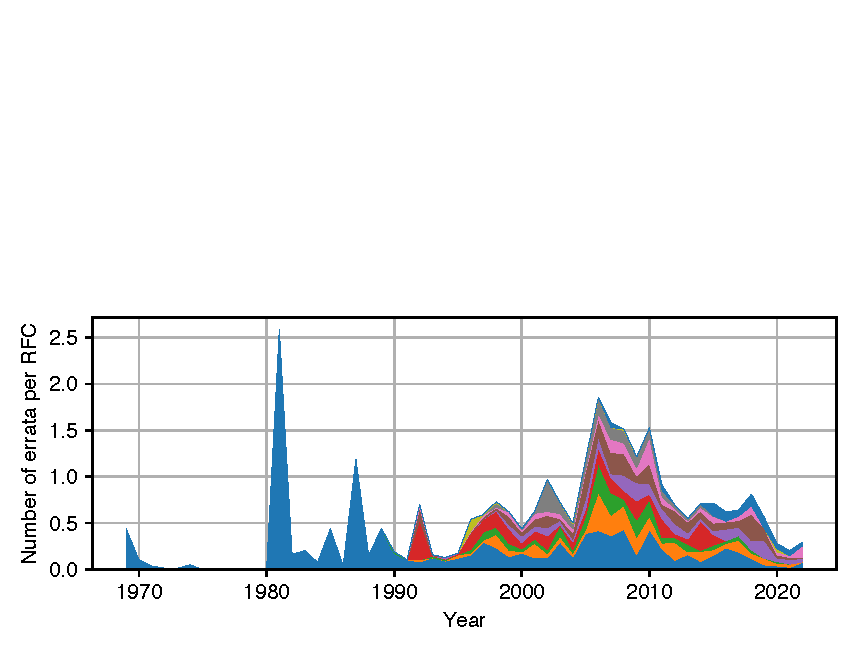
\includegraphics[width=\figureWidthOneColumn]{figures-prev/tma-2023/errata-by-year.pdf}
  \caption{
    Average number of errata filed per RFC in each year, by RFC publication year,
    grouped by IETF area. The areas are as described in Figure~\ref{fig:rfcs_by_area}.
  }
  \label{fig:errata_per_year}
\end{figure}

\begin{table*}
\centering
\footnotesize
\begin{tabular}{rlrrr}
\toprule
\textbf{RFC} & \textbf{Title} & \textbf{Year} & \textbf{Area} & \textbf{Filing count} \\
\midrule
4601 & Protocol Independent Multicast - Sparse Mode (PIM-SM): Protocol Specification (Revised) & 2006 & rtg & 114 \\
4880 & OpenPGP Message Format & 2007 & sec & 52 \\
793 & Transmission Control Protocol & 1981 & None & 47 \\
4634 & US Secure Hash Algorithms (SHA and HMAC-SHA) & 2006 & None & 44 \\
5661 & Network File System (NFS) Version 4 Minor Version 1 Protocol & 2010 & tsv & 42 \\
1345 & Character Mnemonics and Character Sets & 1992 & app & 41 \\
8446 & The Transport Layer Security (TLS) Protocol Version 1.3 & 2018 & sec & 40 \\
5545 & Internet Calendaring and Scheduling Core Object Specification (iCalendar) & 2009 & app & 35 \\
3261 & SIP: Session Initiation Protocol & 2002 & rai & 33 \\
5905 & Network Time Protocol Version 4: Protocol and Algorithms Specification & 2010 & int & 32 \\
\bottomrule
\end{tabular}
\caption{Top 10 RFCs by errata filing count}
\label{tab:top-10-rfcs-by-errata}
\end{table*}

\begin{table*}
\centering
\footnotesize
\begin{tabular}{lr|rrrr|rr}
\toprule
\textbf{Area} & \textbf{\#} & \textbf{Verified} & \textbf{Held} & \textbf{Rejected} & \textbf{Reported} & \textbf{Technical} & \textbf{Editorial} \\
\midrule
None & 1883  & 895  & 505  & 197  & 286  & 930  & 953 \\
Internet (int) & 650  & 281  & 223  & 98  & 48  & 342  & 308 \\
Operations and Management (ops) & 558  & 311  & 113  & 67  & 67  & 297  & 261 \\
Real-time Applications and Infrastructure (rai) & 457  & 143  & 213  & 48  & 53  & 255  & 202 \\
Security (sec) & 888  & 291  & 265  & 115  & 217  & 447  & 441 \\
Routing (rtg) & 831  & 305  & 378  & 140  & 8  & 326  & 505 \\
Applications (app) & 787  & 370  & 175  & 116  & 126  & 464  & 323 \\
Transport (tsv) & 459  & 188  & 142  & 75  & 54  & 258  & 201 \\
General (gen) & 41  & 22  & 4  & 5  & 10  & 8  & 33 \\
Applications and Real-Time (art) & 204  & 64  & 32  & 16  & 92  & 143  & 61 \\
Sub-IP (subip) & 1  & 1  & 0  & 0  & 0  & 1  & 0 \\
\midrule All & 6759  & 2871  & 2050  & 877  & 961  & 3471  & 3288 \\
\bottomrule
\end{tabular}
\caption{Errata statistics by area.}
\label{tab:errata-stats-area}
\end{table*}


%..................................................................................................
\pb{Errata Delay:}
We next explore how long it takes for errata to be identified and filed.
Figure~\ref{fig:errata_submission_days} presents a CDF of the number of
days between RFC publication and the errata being filed, broken down based
on IETF area. We see a wide range of delays. 7.3\% of errata are filed
within the first 30 days, suggesting that many RFCs are published with
issues that could have been identified prior to publication.  RFCs from the
General (\emph{gen}) area--describing IETF policies and procedures--have
the longest delay, with a median of 3,458 days, compared to the
Applications and Real-time (\emph{art}) area with a median of 681
days.\footnote{Errata are filed against RFCs within the \emph{subip} area
within a median of 48 days, but this is skewed, with only 19 RFCs being
published in that area.} Editorial errata are typically filed more quickly,
with a median of 987 days, compared to a median of 1,138 days for technical
errata. 


\begin{figure}
  \centering
  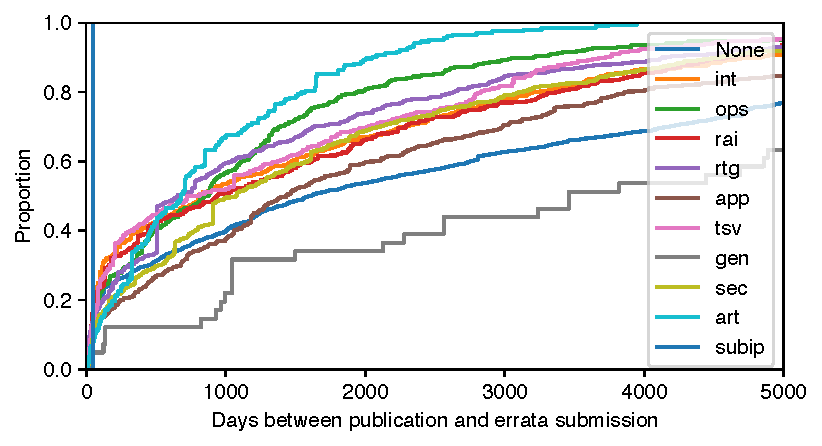
\includegraphics[width=\figureWidthOneColumn]{figures-prev/tma-2023/errata-submission-dates-area.pdf}
  \caption{
    Cumulative distribution of the number of days from RFC publication to
    errata filing by IETF area.
    The areas are as described in Figure~\ref{fig:rfcs_by_area}.
  }
  \label{fig:errata_submission_days}
\end{figure}


%..................................................................................................
\pb{Errata Status:}
Figure~\ref{fig:errata_status} categorises the errata by verification
status and publication year of the RFC to which they relate. 
The largest share (42.5\%) of errata are \emph{verified}: errata that have
been has been confirmed as necessary and accurate. This suggests that many
errata identify real problems with RFCs and are useful to the community.


\begin{figure}
  \centering
  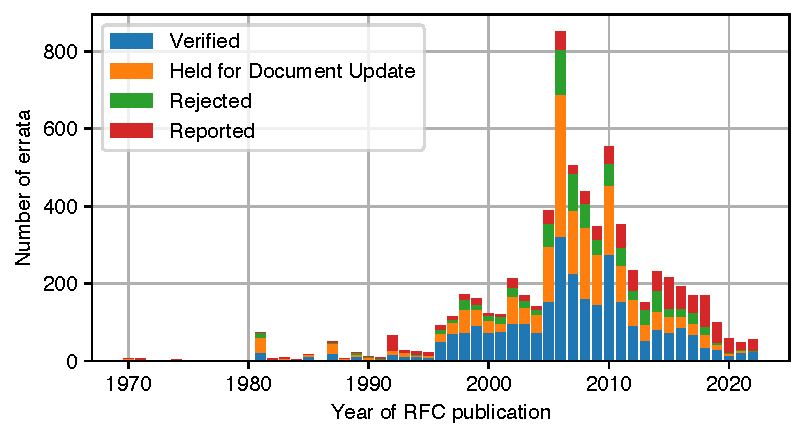
\includegraphics[width=\figureWidthOneColumn]{figures-prev/tma-2023/errata-by-status.pdf}
  \caption{
    Errata filings by status, by publication year of the RFC.
  }
  \label{fig:errata_status}
\end{figure}

The next largest share (30.3\%) are those labelled \emph{hold for document
update}.  These are errata that are not a necessary update to the RFC, but
may be considered on future revisions. For example, \emph{erratum 6278}
describes an oversight in RFC 8610~\cite{RFC8610}; the solution to this is
non-trivial, and so will be considered in the next version of the
specification. Of the 930 RFCs that have \emph{hold for document update}
errata filed against them, only 40\% have been updated or obsoleted by a
subsequent RFC.  We flag that this may be a cause for concern, or at least
a missed opportunity for improvements to standards.

The third largest category (13\%) is \emph{rejected}, which covers errata
that are invalid (like \emph{erratum 6323}, which was rejected because the
original text was understood to be correct) or proposes a significant
change to the RFC that should be done by publishing a new RFC (like
\emph{erratum 5814}, which was rejected for proposing a significant change,
rather than reporting an error). Such a large fraction of rejected
submissions is unexpected and may flag issues with people's understanding
of the errata process and its place within the wider standardisation
process.

Finally, 14.2\% of errata are \emph{reported} but unverified.  Again, we
are surprised to see unverified errata from over a decade ago, suggesting
the process should be expedited. 


%..................................................................................................
\pb{Errata per RFC Area, Status, and Stream:}
Figure~\ref{fig:errata_per_rfc} shows a CDF of the number of errata filed,
per RFC, in each IETF area. Non-IETF RFCs, e.g., IRTF and independent stream
RFCs, and legacy IETF RFCs, are labelled as ``None''.  We confirm errata in
standards are common: of the 4,373 standards-track RFCs in our dataset,
32.7\% have attracted at least one erratum filing.  However, there are
three notable outliers:
\begin{enumerate}
  \item RFCs published by the Sub-IP (subip) Area have very few errata,
    with only 5\% of subip RFCs attracting errata filings. This temporary
    area -- established in 2001 and concluded in 2005 -- only published 19
    RFCs, resulting in a far smaller sample than the other areas. For
    comparison, the next smallest area, General (gen), published 39 RFCs.
    \emph{gen} RFCs attract a greater number of errata on average, vs.
    \emph{subip} RFCs, likely due to their broader relevance.  

  \item We see that both the Application (app) and Security (sec) Area
    RFCs are more likely to have errata filed for them than other areas,
    with 35.9\% of Application and 39\% of Security RFCs attracting at
    least one erratum filing.

  \item Table~\ref{tab:errata-stats-area} details the split between
    \emph{technical} and \emph{editorial} errata across each area.  While
    there is broadly an even split, there are areas where one type of
    errata is more dominant. For example, in the Routing (rtg) area, 60.8\%
    of filings are editorial, while in the Applications (app) area, 59\%
    were technical.  It remains to determine why this is the case, and, in
    particular, to establish whether there is something inherent about the
    RFCs published by these areas that makes them more prone to containing
    errata, and to containing one type of errata vs. another. For example,
    in the Routing area, structured notation is frequently used to define
    routing entities; editorial errata are often filed in those
    definitions. Targeting such areas with improved alternate review
    procedures may be beneficial.

\end{enumerate}

\begin{figure}
  \centering
  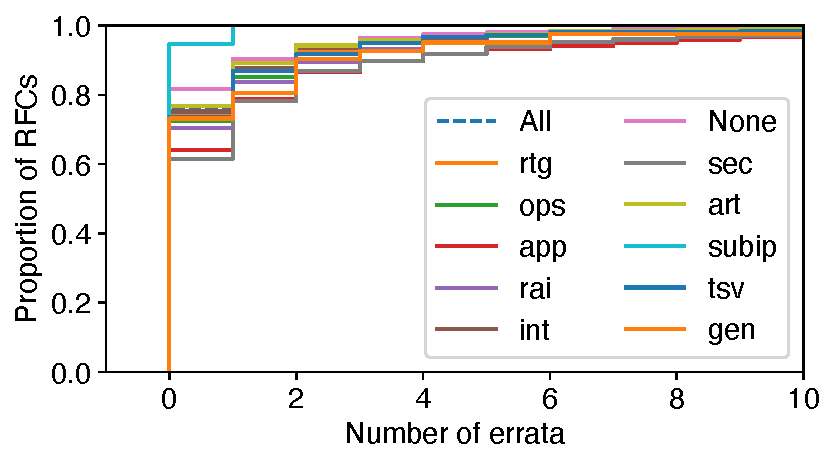
\includegraphics[width=\figureWidthOneColumn]{figures-prev/tma-2023/errata-by-rfc-by-area.pdf}
  \caption{
    Cumulative distribution of errata filed per RFC by grouped by IETF
    area.  The areas are as described in Figure~\ref{fig:rfcs_by_area}.
  }
  \label{fig:errata_per_rfc}
\end{figure}

Tables~\ref{tab:errata-stats-stream} and \ref{tab:errata-stats-status}
further categorise errata by the stream and status, at the time of
publication, of each RFC. As expected, the majority of errata are filed
against IETF RFCs and \emph{Proposed Standards} since these make up the
majority of RFCs that are published. However, there are notable differences
in the average number of filings per RFC. \emph{Proposed Standards} (1.01
errata per RFC), \emph{Draft Standards} (1.93), and \emph{Internet
Standards} (2.17) attract a far higher number of errata per RFC than
\emph{Informational} (0.52) or \emph{Experimental} (0.39) documents. This
may be due to the additional readership and attention that standards-track
documents receive, and because they are more likely to be the basis for
future work and protocol extensions.

\begin{table*}
\centering
\footnotesize
\begin{tabular}{lr|rrrr|rr}
\toprule
\textbf{Stream} & \textbf{\#} & \textbf{Verified} & \textbf{Held} & \textbf{Rejected} & \textbf{Reported} & \textbf{Technical} & \textbf{Editorial} \\
\midrule
IETF (6619) & 5797  & 2348  & 1815  & 798  & 836  & 3034  & 2763 \\
IAB (124) & 55  & 25  & 13  & 3  & 14  & 23  & 32 \\
Independent (376) & 330  & 235  & 32  & 28  & 35  & 172  & 158 \\
Legacy (1929) & 510  & 226  & 182  & 39  & 63  & 198  & 312 \\
IRTF (97) & 67  & 37  & 8  & 9  & 13  & 44  & 23 \\
\midrule All & 6759  & 2871  & 2050  & 877  & 961  & 3471  & 3288 \\
\bottomrule
\end{tabular}
\caption{Errata statistics by stream; the ``\emph{Editorial}'' stream has no documents, and is not shown.}
\label{tab:errata-stats-stream}
\end{table*}

\begin{table*}
\centering
\footnotesize
\begin{tabular}{lr|rrrr|rr}
\toprule
\textbf{Status} & \textbf{\#} & \textbf{Verified} & \textbf{Held} & \textbf{Rejected} & \textbf{Reported} & \textbf{Technical} & \textbf{Editorial} \\
\midrule
Proposed Standard (4084) & 4142  & 1680  & 1308  & 555  & 599  & 2213  & 1929 \\
Informational (2894) & 1500  & 719  & 399  & 136  & 246  & 754  & 746 \\
Internet Standard (147) & 319  & 118  & 111  & 66  & 24  & 135  & 184 \\
Best Current Practice (316) & 233  & 111  & 53  & 30  & 39  & 80  & 153 \\
Historic (70) & 20  & 13  & 4  & 2  & 1  & 9  & 11 \\
Draft Standard (142) & 274  & 94  & 93  & 66  & 21  & 150  & 124 \\
Experimental (563) & 221  & 115  & 65  & 20  & 21  & 121  & 100 \\
Unknown (929) & 50  & 21  & 17  & 2  & 10  & 9  & 41 \\
\midrule All & 6759  & 2871  & 2050  & 877  & 961  & 3471  & 3288 \\
\bottomrule
\end{tabular}
\caption{Errata statistics by status at publication.}
\label{tab:errata-stats-status}
\end{table*}


% \todo{Should we include ``Impact of Citations'' from TMA 2023?}

%..................................................................................................
\pb{Errata Location:}
Finally, we investigate the location of errata within RFCs.
Figure~\ref{fig:errata_location_percent_count} presents the number of
errata occurring at each decile of the documents, for the 2,552 filings
where accurate location information is available, and after the copyright
notice and other boilerplate has been removed.  We see that technical
errata dominate over editorial in almost all places, except for the very
beginning where the \textit{Introduction} is located. Moreover, it shows
that the most technical errata are near the middle of the document where
the most complex content is.  We explore where errata occur, with
Figure~\ref{fig:errata_section_wise_counts} showing section titles for
errata appearing in at least $10$ documents. Sections such as the
\emph{Introduction} or \textit{References} are dominated by editorial
errata while more technical sections, like \emph{IANA Considerations} (i.e.,
parameter registrations), \emph{Security Considerations} or
\emph{Definitions}, have a larger proportion of technical errata. In
addition, we see that sections labelled \emph{Appendix} attract a
significant proportion of technical errata. While appendices vary in their
content, they are widely used to provide pseudocode and test vectors, or to
describe algorithms. This suggests that it may be useful to target review
efforts on appendices and other dense technical content where errata are
more likely.

\begin{figure}
  \centering
  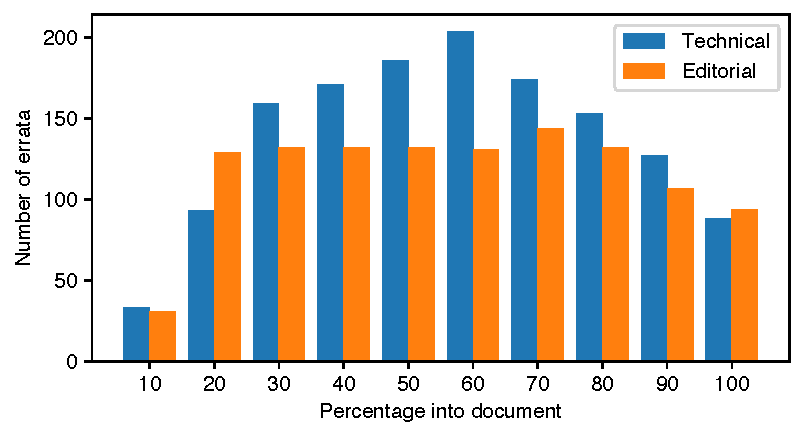
\includegraphics[width=\figureWidthOneColumn]{figures-prev/tma-2023/location-percent.pdf}
  \caption{
    Errata counts by percentile location in document (0 is the beginning;
    100 is the end).
  }
  \label{fig:errata_location_percent_count}
\end{figure}

\begin{figure}
  \centering
  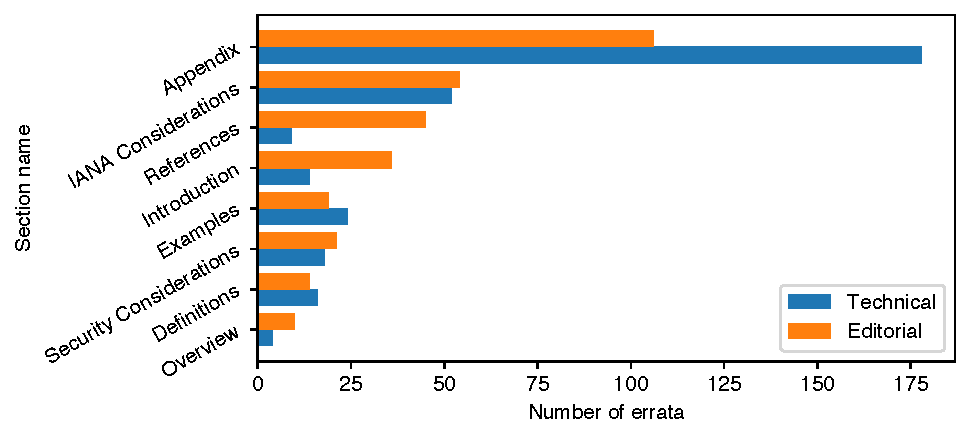
\includegraphics[width=\figureWidthOneColumn]{figures-prev/tma-2023/section-title-counts.pdf}
  \caption{
    Errata counts by section title for the more frequent section titles.
  }
  \label{fig:errata_section_wise_counts}
\end{figure}

%--------------------------------------------------------------------------------------------------
\subsection{Summary}

On RFC Production and Complexity (\S\ref{sec:trends-documents:production})
we see evidence that Internet standards are maturing and that the pace of
innovation has slowed. The rate of standards publication peaked in the
mid-2000s, and has gradually declined since, and the number of IETF working
groups has also started to decline. The standards that are being produced
are taking longer, with more revisions prior to publication, and make
increasing use of normative language and references to prior work; all
evidence of complexity and the burden of backwards compatibility. The signs
are that the IETF has developed, and is maintaining and extending, the core
Internet standards, but has not broken out of that niche to new topic areas.


The RFC errata (\S\ref{sec:trends-documents:errata}) process seems to be
broadly effective at finding problems, although there are a concerning
number of unresolved errata reports that are perhaps indicative of an
organisation that doesn't effectively maintain supposedly completed work.
The high prevalence of errata in security-related RFCs also deserves
further scrutiny to determine whether it is due to a higher number of
defects in these RFCs or because defects are more likely to be noticed
because these RFCS receive more review.


%==================================================================================================
\section{Trends in Participant Demographics}
\label{sec:trends-demographics}

In this section, we look at the authorship of published RFCs to explore
how participation in the IETF has changed over time. We show that the
geographic distribution of RFC authors has shifted over time, with the
proportion of authors from the US decreasing and a corresponding rise in
authors from Europe and China (\S\ref{sec:trends-demographics:geographic}).
We similarly explore shifts in affiliation, showing increasing influence of
Huawei and ongoing shifts in the fortunes of many prominent US and European
technology companies (\S\ref{sec:trends-demographics:affiliation}). The
ongoing influence of Cisco and strong input from academic institutions is
also noted.

% The following is from our IMC 2021 paper, Section 3.2.

%--------------------------------------------------------------------------------------------------
\subsection{Geographic Distribution of Authors}
\label{sec:trends-demographics:geographic}

The IETF Datatracker maintains metadata about document authors, including
their names, email addresses, affiliations, and location information. This
dataset does not cover the entire RFC corpus, with metadata available for
authors of RFCs published from 2001, and where it has been provided country
data is available for around 70\% of authors, while affiliation information
is provided for around 80\% of authors. 

Figure~\ref{fig:author_countries_normalised} shows how the proportion of
RFC authors from different countries varies over time, with Figure
\ref{fig:author_continents_normalised} breaking this down by continent.
The IETF has signalled that it wishes to encourage greater geographical
diversity~\cite{RFC7704,ietfblog:diversity}.  Without an explicit goal, we
frame our findings within the context of global population distribution.
We find that North America, while still disproportionately over represented,
is becoming less dominant.  75\% of authors were from North America in 2001,
and this has declined to 44\% in 2020. At the same time, representation of
both Europe and Asia has grown, from 17\% to 40\% and 6\% to 14\%, respectively.
However, Africa and South America remain heavily under-represented, with
only $\approx$0.5\% of authors coming from either continent in 2020.  This
suggests that, if the IETF is to become more geographically representative,
further efforts are needed.

\begin{figure}
  \centering
  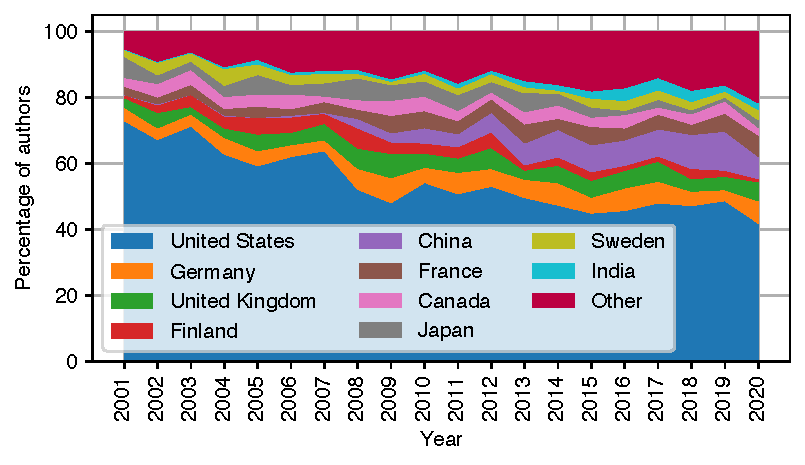
\includegraphics[width=\figureWidthOneColumn]{figures-prev/imc-2021/authors/top5_countries_normalised.pdf}
  \caption{
    Authorship countries (normalised)
  }
  \label{fig:author_countries_normalised}
\end{figure}

\begin{figure}
  \centering
  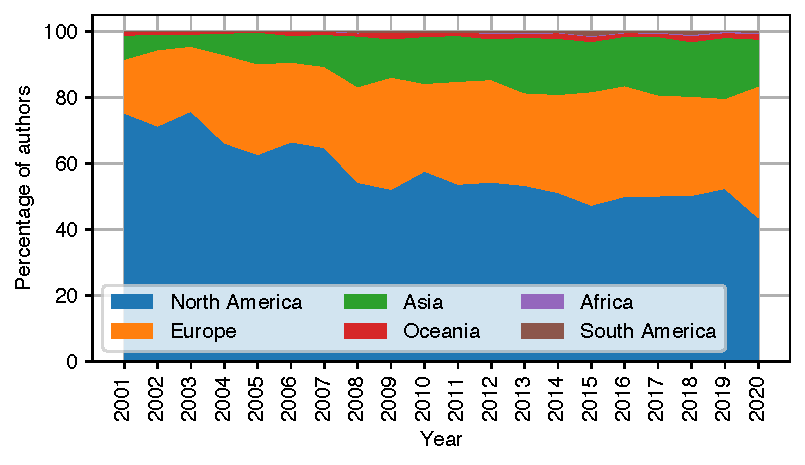
\includegraphics[width=\figureWidthOneColumn]{figures-prev/imc-2021/authors/continents_normalised.pdf}
  \caption{
    Authorship continents (normalised)
  }
  \label{fig:author_continents_normalised}
\end{figure}

%--------------------------------------------------------------------------------------------------
\subsection{Author Affiliations}
\label{sec:trends-demographics:affiliation}

To explore trends in author affiliations, we gather affiliation data from
the IETF Datatracker.  This data is processed to normalise affiliation
names by removing common variations in spelling and to amalgamate known
subsidiaries and merged companies. For example, Huawei and Futurewei are
combined as Huawei, and Sun Microsystems is merged with Oracle.

%..................................................................................................
\pb{Corporate Authors:}
Figure~\ref{fig:author_affiliations_normalised} shows the top ten
affiliations by proportion of RFC authors each year. We observe several
interesting trends.  First, Cisco remains a consistent employer of IETF
contributors, with around 12\% of authors affiliated with the company in
2020, and having been the single largest affiliation across all years in
the dataset. We can also see the rise of Huawei beginning in 2005, with
7.1\% of authors being affiliated with the company in 2020, having peaked
at 9.7\% in 2018. Google has a similar trajectory, first appearing in the
dataset in 2006, with 3.8\% of authors being affiliated with it in 2020.

We also observe the decline of a number of affiliations.  Microsoft and
Nokia, having peaked with 3.3\% and 3.6\% of authors, had 0.7\% and 1.7\%
of authors in 2020, respectively, with the absolute number of authors from
both companies also declining.

These shifts in affiliation reflect changes in fortune and commercial
success of the companies. They also show the ongoing importance of IETF
standards, with new companies choosing to send participants: while we do
not demonstrate any causal link, it is encouraging that commercially
successful companies opt to enable their employees to actively participate
in the IETF. Care is needed to ensure that this relevance is maintained,
however: we observe that the author pool has grown less diverse in terms of
companies that are represented. 35.4\% of authors came from the top 10
affiliations in the dataset in 2020, compared with 25.6\% in 2001. 


\begin{figure}
  \centering
  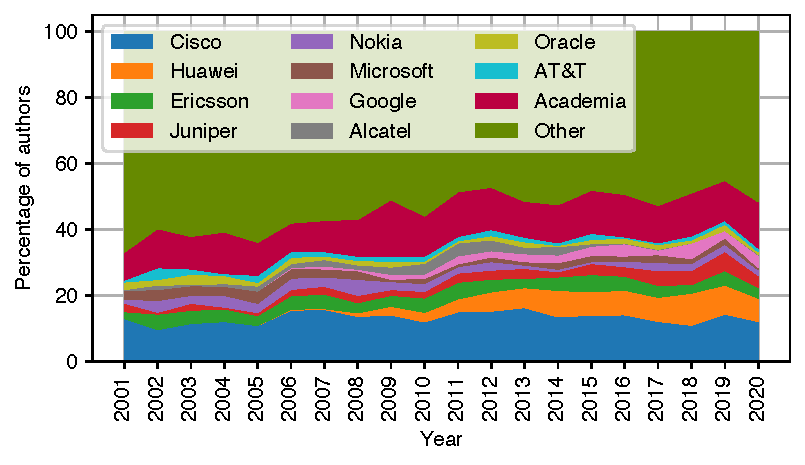
\includegraphics[width=\figureWidthOneColumn]{figures-prev/imc-2021/authors/top5_affiliations_normalised.pdf}
  \caption{
    Authorship affiliations (normalised)
  }
  \label{fig:author_affiliations_normalised}
\end{figure}

%..................................................................................................
\pb{Academia and consultants:}
Academic affiliations are those where the affiliation name contains
``University'', ``Institute'', or ``College'', while consultancy
affiliations are those that contain ``Consultant`` (we recognise that this
definition of consultants is limited and incomplete). Affiliation data has
been normalised to remove common abbreviations (e.g., ``U.'' for
``University'') and to translate non-English affiliations.  As shown in
Figure~\ref{fig:author_affiliations_normalised}, we find that an increasing
number of authors come from academic affiliations, growing from 8.1\% of
authors in 2001, to 13.6\% in 2020, having peaked at 16.5\% in 2009. The
number of consultants, by our limited measure, has remained stable,
accounting for 2\% of authors in 2020.  The remaining authors are largely
from industrial affiliations.

Figure~\ref{fig:author_affiliations_normalised_acad} shows the top 10
academic affiliations in the dataset, and the percentage of academic
authors that have those affiliations over time. In general, academic
affiliations are each typically held by a small number of authors. We can
see a number of trends in academic authorship, with fewer authors from
Columbia University, MIT, and ISI in recent years, and the rise of Tsinghua
University.

While some academic affiliations are shared by large groups of participants
(e.g., MIT, ISI, Tsinghua University), academic participation is often
driven by a single research group or individual within an institution.
This allows smaller institutions, such as the University of Bremen and
the University of Auckland, that appear in Figure~\ref{fig:author_affiliations_normalised_acad},
and others with single but prolific authors, to have outsize influence.
Understanding whether this indicates academics pushing for standardisation
of the results of government funded research to increase its impact, the
outcomes of industry sponsored research, or academics acting as consultants
for industry, is for further study.

\begin{figure}
  \centering
  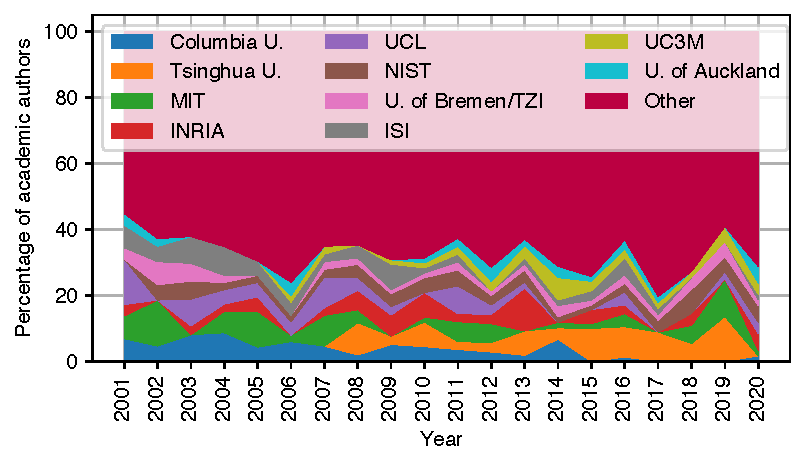
\includegraphics[width=\figureWidthOneColumn]{figures-prev/imc-2021/authors/top5_affiliations_normalised_acad.pdf}
  \caption{
    Academic affiliations (normalised)
  }
  \label{fig:author_affiliations_normalised_acad}
\end{figure}

%..................................................................................................
% IMC 2021 paper Section 3.2 (last part)
\pb{Arrival of new authors:}
Figure~\ref{fig:author_new} shows the percentage of authors in each year
that have not previously authored an RFC. Given that the dataset used here
begins in 2001, 100\% of authors are new in that year. The more stable
trend in recent years likely highlights the churn in RFC authorship, with
around 30\% of authors each year having never previously authored an RFC.
This is consistent with the presence of authors with new affiliations
and from new countries and shows an ongoing influx of new participants.

\begin{figure}
  \centering
  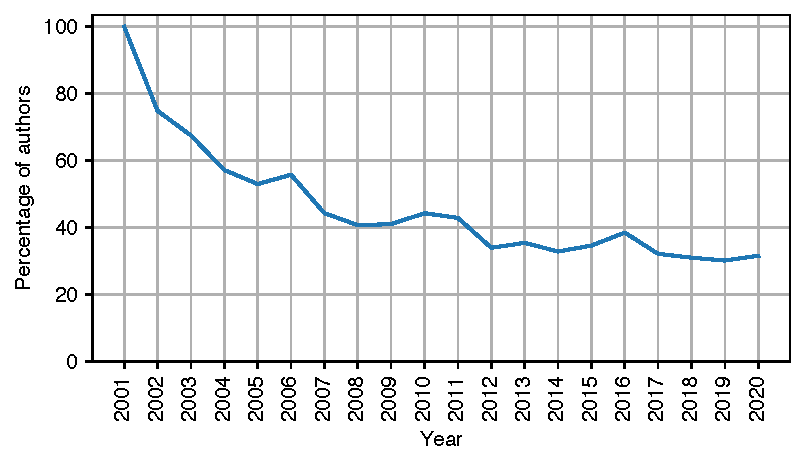
\includegraphics[width=\figureWidthOneColumn]{figures-prev/imc-2021/authors/repeat_authors.pdf}
  \caption{
    Percentage of new authors per year.
  }
  \label{fig:author_new}
\end{figure}

%--------------------------------------------------------------------------------------------------
\subsection{Summary}
The trends highlighted in this section  indicate a pool of authors that is
slowly diversifying and changing over time, with a growing proportion of authors
from outside of North America, contributions from new companies and
affiliations, and relatively high authorship churn. Despite this, we find
that certain regions and groups are not well represented in the IETF (e.g.,
contributors from Africa), and that the authorship pool is becoming
increasingly centralised, with a third of authors coming from the top 10
affiliations. This suggests that, if the IETF is concerned with being
more representative, further efforts are needed.


%==================================================================================================
\section{Organisational Dynamics of the IETF}
\label{sec:org-dyn}

While the IETF does hold regular plenary and interim meetings, much of the
interaction between participants takes place on the public mailing lists of
the various working groups. In the following (\S\ref{sec:org-dyn:participants}),
we characterise the mailing list interactions considering the volume of
discussion, the number of drafts discussed, the duration of individual
participation, and how interactions between participants change over time.

We then consider influence and impact of participants (\S\ref{sec:org-dyn:influence}).
We measure how centralised is the active IETF community and how reliant is
it on a small core of participants; how the most influential participants
behave; how influence, determined by mailing list participation, relates to
wider impact in the IETF; and whether the organisational affiliation of
participants influences adoption of new work.

Finally, we consider the hierarchy and communication dynamics in the IETF
(\S\ref{sec:org-dyn:hierarchy}). We ask whether participation in IETF
leadership roles is growing or becoming more centralised onto a small group
of participants; whether the formal organisational hierarchy is reflected
in the patterns of communication between participants; how people in
different roles communicate and whether information flows up or down the
hierarchy; and whether contact with people in leadership positions
influences mobility within the IETF.

%--------------------------------------------------------------------------------------------------
\subsection{Characterising Participant Interactions}
\label{sec:org-dyn:participants}

% IMC 2021 paper Section 3.3

The operations of the IETF is largely underpinned by mailing list
interactions, which are used to discuss and finalise the drafts that
eventually become RFCs. Our data, which starts from 1995, confirms their
vital role, with 1,153 mailing lists, containing 2,439,240 emails from
74,646 unique email addresses.

\pb{Volume of Discussion:}
Figure~\ref{fig:pid_count_emailing_yearly} shows the number of emails sent
across the last 25 years (dashed red line), showing that email volumes have
grown significantly with time, plateauing at around 130,000 messages per
year since around 2010. The figure also shows (solid blue line) how the
number of unique participants (with entity resolution performed as
discussed in Section \ref{sec:background:data}) observed every year in the
mail lists, showing a decreasing trend in the number of contributors since
2007. We note that the number of participants is broadly correlated
with the rate of RFC publication (Figure \ref{fig:rfcs_by_area}), likely
indicating that many participants disengage once the document they were
working on is published.

\begin{figure}
  \centering
  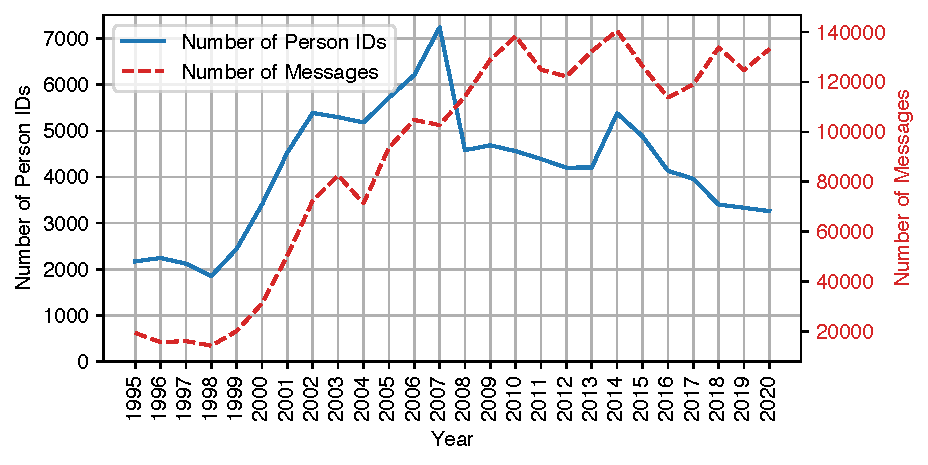
\includegraphics[width=\figureWidthOneColumn]{figures-prev/imc-2021/emails/pid_count_emailing_yearly.pdf}
  \caption{
    Number of email messages per year and number of unique participants
    exchanging emails per year.
  }
  \label{fig:pid_count_emailing_yearly}
\end{figure}

Figure~\ref{fig:emailvol_by_year_catg} breaks down the messages sent into
four categories based on the sending address:
\begin{enumerate}
  \item \emph{Datatracker-mapped} addresses represent those participants
    sending email in a given year that have an IETF Datatracker account
    associated with their email address. Datatracker accounts are needed to
    submit drafts and register for meetings, and to allow those in
    leadership roles to perform administrative actions, so this indicates
    the fraction of participants who are strongly engaged with the IETF.

  \item \emph{Automated} addresses are those sent by automated systems
    rather than directly by participants. This includes the automated
    announcement of new draft submissions and meeting, last calls for
    comments, etc., sent by the Datatracker, but there is also a growing
    number messages sent by GitHub and other version control systems used
    for managing drafts.
    There were 122 active IETF working groups at the time of writing.
    Of these, 17 listed a GitHub repository in their metadata. The QUIC
    working group, as one example, has replaced the typical email list
    discussions with GitHub issues: indeed, this is a significant part of
    the surge observed in 2016.  Given that most working groups use mailing
    lists to manage their activity, we do not further analyse interactions
    that take place on GitHub. 

  \item \emph{Role-based} addresses represent those sent by people in
    formal leadership or administrative roles in the context of their role.
    There are a very limited number of these addresses, e.g., the IETF,
    IRTF, and IAB Chairs, the IETF Executive Director. As seen, these
    addresses are used sparingly. Note that working group chairs and area
    directors use their individual email addresses when managing their
    working group or area, and so appear as Datatracker mapped addresses.

  \item \emph{Unmapped} addresses are those that do not fall into the other
    categories. They typically represent participants that lurk on a
    mailing list and provide occasional input, but who are not document
    authors and do not attend meetings. This category has reduced over time
    as more types of interaction require a Datatracker account and as
    comments from occasional contributors are increasingly submitted via
    issue trackers on GitHub and similar services.

\end{enumerate}

The increasing use of GitHub suggests that the data in
Figure~\ref{fig:pid_count_emailing_yearly} likely understates the volume of
interactions. The plateau observed in the number of messages sent in recent
years is at least somewhat attributable to the shift to GitHub and similar
services. As this shift continues, it will become important for future work
to consider these interactions.

\begin{figure}
  \centering
  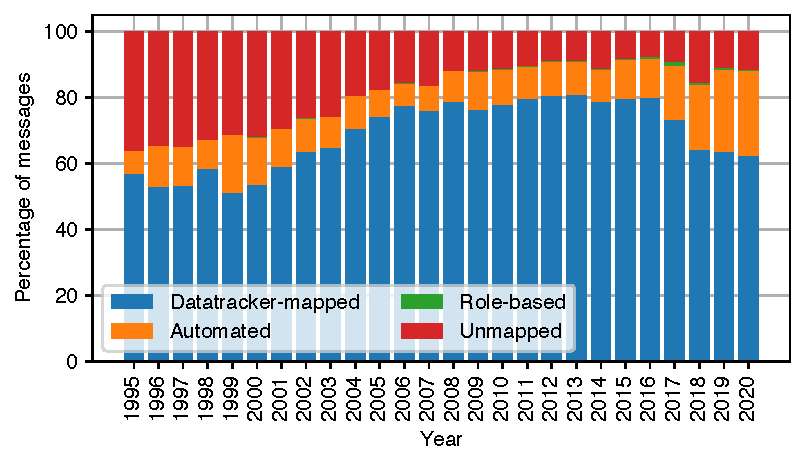
\includegraphics[width=\figureWidthOneColumn]{figures-prev/imc-2021/emails/frequency_emails_yearly_categories2.pdf}
  \caption{
    Number of messages exchanged per year across different categories:
    messages mapped to the Datatracker (Datatracker Person-ID); messages
    by automated email addresses (Automated); messages by role-based
    addresses (Role-based); and messages not mapped to the Datatracker
    (New Person-ID)
  }
  \label{fig:emailvol_by_year_catg}
\end{figure}

%..................................................................................................
\pb{Discussion of draft documents:}
The mailing lists are, other than plenary or interim meetings, the primary
means for the discussion of draft documents. To measure how often drafts are
discussed, we identify mentions of Internet-Drafts and RFCs in mailing list
messages.  We extract any mention of a draft (beginning \texttt{draft-}) or
RFC (i.e., ``RFC'' followed by a number).  Figure~\ref{fig:draft_mentions}
presents the number of drafts mentions in the emails per year. Separate
mentions of the same draft are counted as different mentions, as we want to
observe the entire volume of mentions.  We observe a strong increase in the
number of mentions over time.  

% This is largely driven by the growing number of drafts being published. In
% fact, we find a Pearson correlation of 0.89 between the number of drafts
% published and the number of mentions. This speaks to the influence of
% emails that mention drafts in driving draft production.

When compared with the number of active drafts (Figure \ref{fig:drafts-by-date}
in \S\ref{sec:trends-documents:production}) we see that the number of mentions
of work-in-progress drafts and RFCs is increasing faster than the number of
such documents. This further supports the hypothesis of increasing standards
complexity---discussion is increasingly referencing prior standards and
other work in progress, as would be expected if the task of ensuring
compatibility with that work is growing in complexity.


\begin{figure}
  \centering
  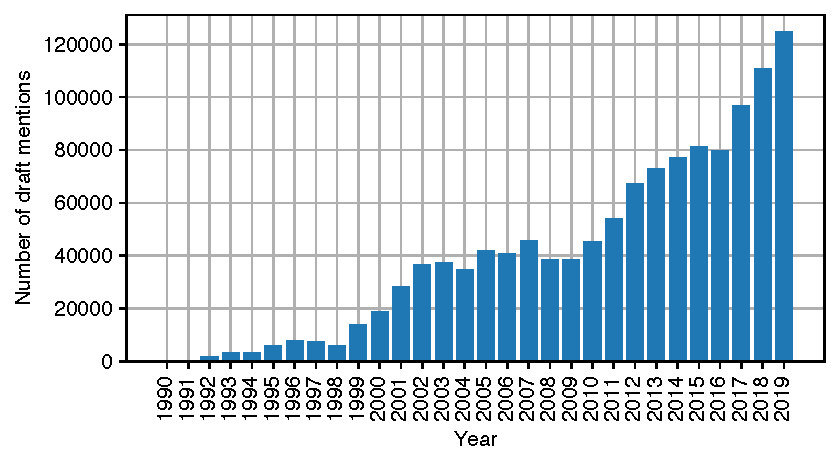
\includegraphics[width=\figureWidthOneColumn]{figures-prev/imc-2021/emails/yearly-draft-mention-volume.pdf}
  \caption{
    Number of mentions of Internet-Drafts and RFC in the IETF email
    archive, per year.
  }
  \label{fig:draft_mentions}
\end{figure}

%..................................................................................................
\pb{Duration of Participation:}
We now look into the duration of participation, in terms of the number of
years that people actively participate in any IETF mailing lists.

We define the \textit{contribution duration} of a participant as the length
of time that they have contributed to the mailing lists.  To do this, we
study the participants who first send email to mailing lists between the
years 2000 to 2013. We limit our analysis to 2013, since the longevity of
contributors that first participate more recently cannot be determined.
For each year, in the period 2000 to 2013, we look at those who first
sent email in each year and the number of years that they then go on to
remain active in the mailing lists. For example, a participant who first
sent an e-mail to an IETF list in 2010, and last sent an e-mail to an IETF
list in 2018, will have a contribution duration of 9 years.

First, to understand duration of participation, we first generate Gaussian
Mixture Models for observing different clusters of the maximum duration of
contribution. These models identified three broad clusters into which the
participants can be categorised: \emph{young contributors} for whom the
time between their first and last emails to the IETF lists in one year or
less; \emph{mid-age contributors} who go onto remain active participants in
the email lists for more than one year, but less than five years; and
\emph{senior contributors} who remain participants in the mailing list for
five or more years.

Next, to begin to understand how contribution duration relates to RFC
authorship, we look at the email interactions of the authors of each RFC.
Specifically, we look at the distribution of the contribution duration of
the authors of RFCs, considering the \emph{mean contribution duration} of
all of the authors of the RFC at the time of publication, the contribution
of the \emph{junior-most author} (the author with the lowest contribution
duration at the time of publication), and the contribution of the
\emph{senior-most author} (the author with the highest contribution
duration at time of publication.  Figure~\ref{fig:age_dist_rfc_authors}
shows the distribution of contribution duration of each of these three
measures. This shows that the majority of junior-most authors have
participated for less than 5 years in the IETF (i.e., they are young or
mid-age contributors), whereas the majority of senior-most authors are
senior contributors who have participated in the IETF for significantly
more than 5 years (in fact, 35\% of authors exceed 15 years of IETF
participation).  This shows that RFCs tend to be authored by a mix of
seniority levels.

% We look at outgoing and incoming interactions with RFC authors in the
% period between the first draft and publication of the RFC. If this period
% is less than two years, we look at the activities of authors for two
% years before the RFC was published.  Interactions are defined from the
% viewpoint of the RFC authors: \emph{outgoing interactions} where an RFC
% author responds to an email from other contributors (i.e., email sent);
% and \emph{incoming interactions} where contributors respond to an email
% by the author (i.e., email received).


\begin{figure}
  \centering
  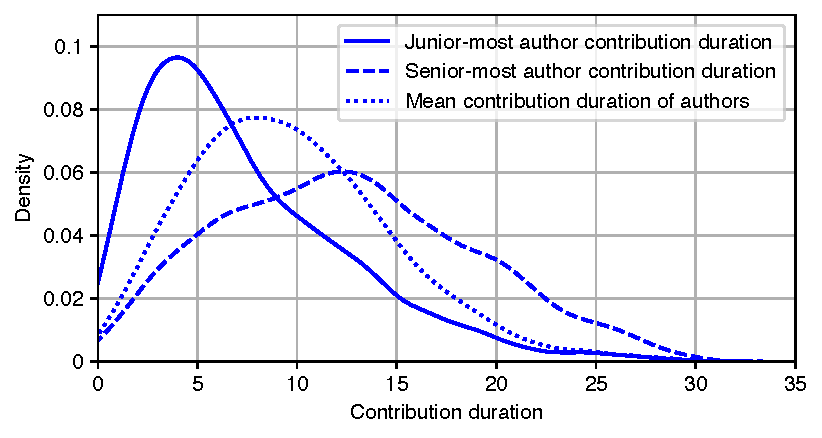
\includegraphics[width=\figureWidthOneColumn]{figures-prev/imc-2021/emails/age_authors_RFCs.pdf}
  \caption{
    Contribution duration distribution of authors of RFCs:
    junior-most author of each RFC, senior-most author of
    each RFC, and mean contribution-duration of all authors
    of each RFC
  }
\label{fig:age_dist_rfc_authors}
\end{figure}

\begin{figure}
  \centering
  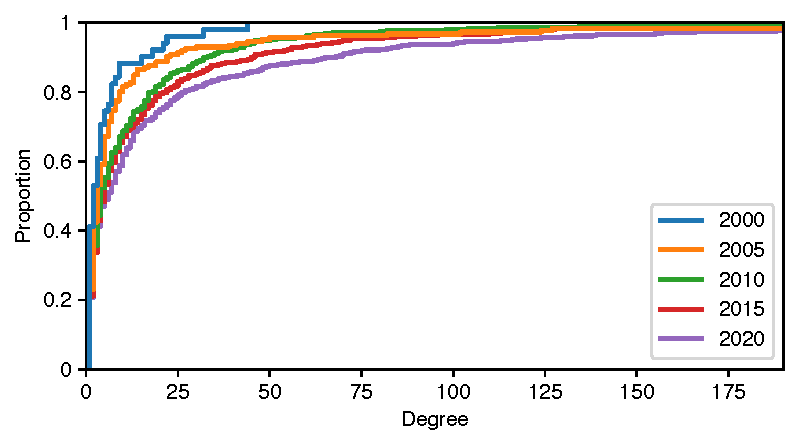
\includegraphics[width=\figureWidthOneColumn]{figures-prev/imc-2021/emails/rfc_authors_degree.pdf}
  \caption{
    CDF showing drift in annual degree (interaction with their network)
    of RFC authors over the period 2000-2020.
  }
  \label{fig:degree_dist_rfc_authors}
\end{figure}

%..................................................................................................
\pb{Evolution of interactions:}
The analysis in Section \ref{sec:trends-documents:production} showed that
RFCs are taking longer to publish and show evidence of increasing complexity.
Such increased complexity should be visible in the email discussion during
preparation of the RFCs.

Figure~\ref{fig:degree_dist_rfc_authors} explores this, showing the change
in the number of other people RFC authors interacte with (i.e., the annual
degree of their communication graph) over time. The amount of interactions
RFC authors engage in has substantially increased over time. For instance,
in the year 2000 only 5.5\% of the authors had a degree of over 25 (i.e.,
they exchanged with more than 25 other people), whereas by the year 2015
almost a quarter of the authors had a degree over 25. This confirms that,
on average, more recent RFCs generate greater discussion. This helps to
explain increasing publication times: as documents become more complex,
authors spend more time interacting with other participants to resolve
the complexity, and these discussions are likely to lead to more drafts.

\begin{figure}
  \centering
  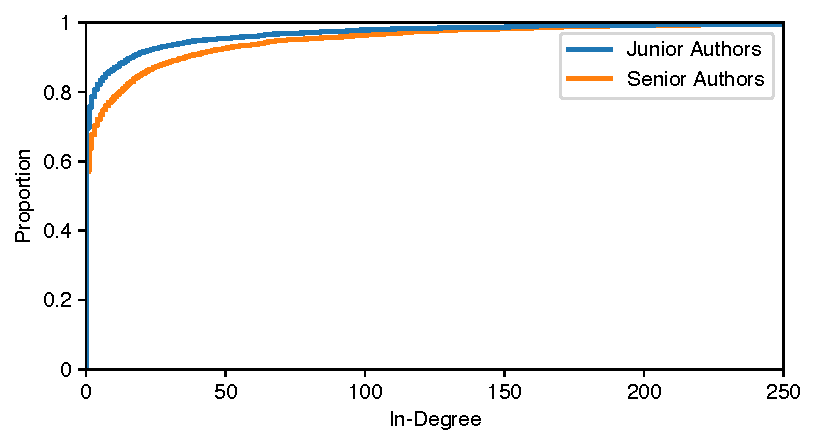
\includegraphics[width=\figureWidthOneColumn]{figures-prev/imc-2021/emails/junior_senior_authors_seniormem_indegree.pdf}
  \caption{
    CDF showing number of senior contributors sending messages (in-degree)
    to junior and senior authors.
  }
  \label{fig:junior_senior_indegree_seniormem}
\end{figure}

We also contrast the interaction patterns of the junior vs.\ senior
authors. Figure~\ref{fig:junior_senior_indegree_seniormem} presents the
CDFs of the in-degree (i.e., number of messages received) across both
junior and senior authors. It shows that the incoming interactions from
senior contributors to junior authors are significantly less than the
incoming interactions from senior contributors to senior authors. Nearly
55\% of junior authors receive messages from fewer than 10 senior
contributors, whereas nearly 65\% of senior authors receive messages from
more than 10 senior contributors.  This speaks to the differing roles
played by these sub-populations: senior authors act as hubs through which
substantial volumes of interaction flow.

%..................................................................................................
\pb{Summary:}
Emails play a vital role in underpinning RFC publication with approximately
130,000 emails sent per year. We have shown that the seniority of both
participants and RFC authors fundamentally changes the volume of
interactions that they have. These trends are likely to have implications
for the IETF community, especially as it tries to encourage new
participants.


%--------------------------------------------------------------------------------------------------
\subsection{Characterising Influence and Impact}
\label{sec:org-dyn:influence}

% ICWSM 2022 paper
% - Measuring influence
% - Behaviour of influential participants
% - Impact of influential participants

% This is modified from the Introduction to the ICWSM 2022 paper:

As we showed in Section \ref{sec:org-dyn:participants}, protocol
standardisation is an inherently social process with most day-to-day work
happening on public mailing lists.  We are specifically
interested in better understanding how influence is distributed across
stakeholders and how it might affect the standardisation process.  This is
of critical societal importance: the IETF has a major impact on global
Internet technologies, and understanding the social processes involved
would give us insight into not only the driving forces behind
standardisation, but also its resilience to the loss of major participants.
In this section we consider the following research questions: 
\begin{enumerate}
  \item How centralised is the active IETF community, and to what extent
    is it reliant on a small core of participants? 
  \item How do the most influential participants behave? 
  \item How does influence (determined by mailing list participation)
    relate to wider impacts throughout the IETF?
  \item Does the organisational affiliation of participants also
    influence the innovation (adoption of new work) within IETF?
\end{enumerate}

% - - - - - - - - - - - - - - - - - - - - - - - - - - - - - - - - - - - - - - - - - - - - - - - - -
\subsubsection{Measuring Influence: The IETF as a Social Graph}
\label{subsec:measuring_influence}

% ICWSM 2022 paper Section 3

To measure influence of participants in the IETF we extend the analysis in
Section \ref{sec:org-dyn:participants} and, for each year, build a social
graph based on the \emph{active community} of participants (nodes) who have
email interactions (edges) with any other participant in the previous five
years. 

We previously demonstrated that there are three categories of participants
in IETF: \textit{young contributors} who leave within one year of their
first year mailing list contribution; \textit{mid-age contributors} who
stay active for up-to five years; and \textit{senior contributors} who
remain active for more than five years (\S\ref{sec:org-dyn:participants}).
Following this, a 5-year period window is chosen to observe interactions.
There are no direct participant-to-participant email exchanges in our
dataset: the emails and responses we capture are sent to the public mailing
lists, and we observe an interaction between two participants when one
replies to an email sent by another on any mailing list. This yields a
social graph based on 1,049,793 emails (out of 2.1M; not all messages
receive a reply) from 22,138 unique participants across 840 mailing lists.

%..................................................................................................
% ICWSM 2022 paper Section 3.1
\pb{Participation}
To examine the variation in participation between IETF participants, in
Figure~\ref{fig:degree_cdf} we plot the cumulative degree distribution
of the social graph (i.e., the cumulative number of people with which a
participant interacts). We observe a core group that always interacts with
substantially more people than the rest of the community, with around 80\%
of the participants interacting with less than 15 others (i.e., having
degree~$<15$), but 5\%-10\% interacting with more than 40 others.
This difference decreases over time: in 2005-2009 only around 6\% of
participants had degree $>$40, but by the period 2015-2019 this increases
to around 10\%.
While there is always a core of more active participants, the amount of
interaction has increased over time.
This confirms the results in Figure \ref{fig:degree_dist_rfc_authors},
for RFC authors, and shows that they also apply to interactions in the
community at large.

\begin{figure}
  \centering
  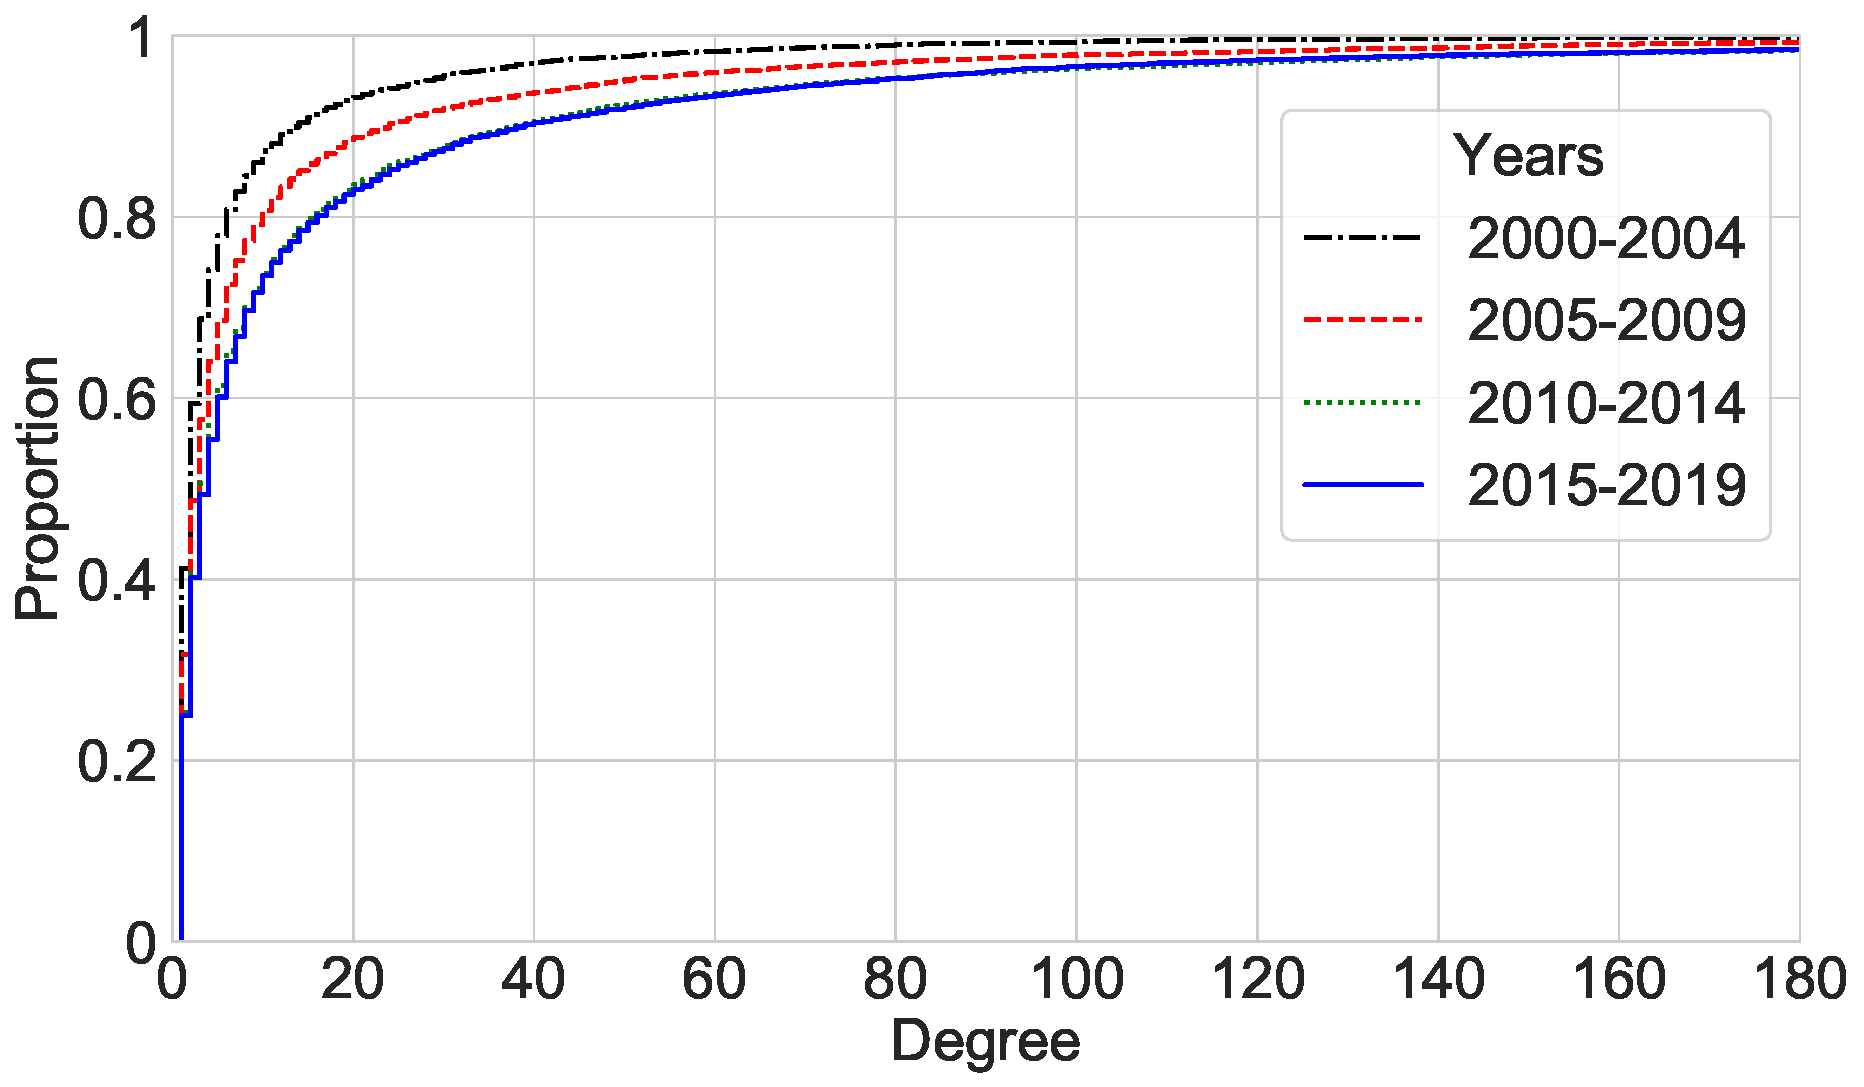
\includegraphics[width=\figureWidthOneColumn]{figures-prev/icwsm-2022/degree_CDF.pdf}
  \caption{
    Cumulative degree distribution of the email graph for different
    year-periods.
  }
  \label{fig:degree_cdf}
\end{figure}

To understand the structure of the community, and its reliance on specific
groups, we analyse the connected components of this graph. Each connected
component reflects a maximal set of nodes such that each pair of nodes is
connected by a path. We compute the size of the Largest Connected Component
(LCC) and the Number of Connected Components (NCC) for each year in
Figure~\ref{fig:lcc_size_yearly}.  The NCC peaks in 2003 before declining,
and broadly aligns with the variation in the number of meeting
attendees,\footnote{\url{https://datatracker.ietf.org/stats/meeting/overview/}}
suggesting a lag between participating for the first time and integrating
into the wider community.  In contrast, the size of the LCC increases until
2006 before stabilising.  Overall, we observe that the IETF community has
become less fragmented over time.

\begin{figure}
  \centering
  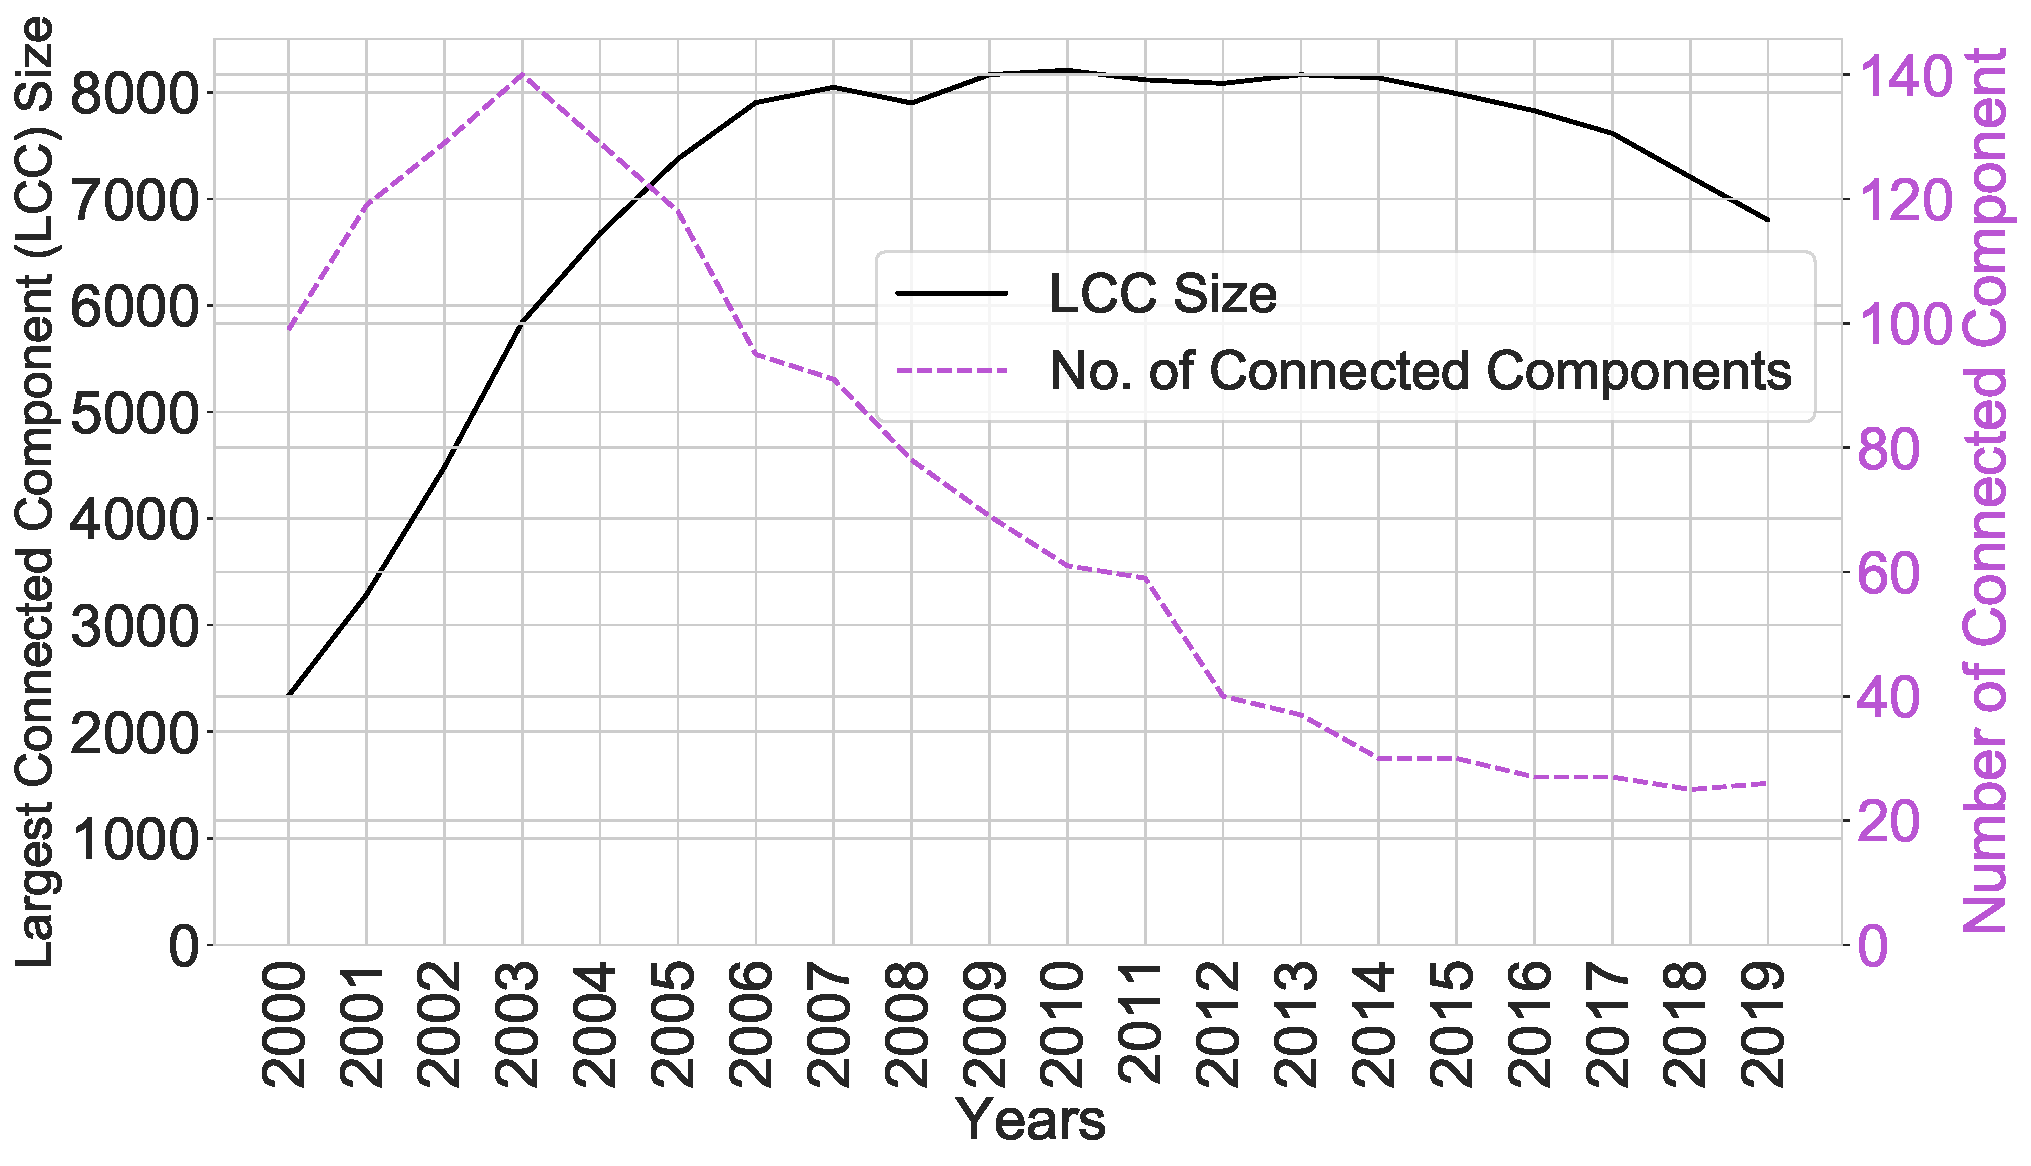
\includegraphics[width=\figureWidthOneColumn]{figures-prev/icwsm-2022/lcc_yearly_no_components.pdf}
  \caption{
    Size of Largest Connected Component (LCC) and Number of Connected
    Components (NCC) of the email graph.
  }
  \label{fig:lcc_size_yearly}
\end{figure}

%..................................................................................................
% ICWSM 2022 paper Section 3.1
\pb{Influence:}
Relying on a small group to interconnect the community could undermine the
resilience of the IETF.  To study the influence of participants and their
role in interconnecting the wider community, we compute the betweenness
centrality of each participant in a given time period
\cite{kourtellis2013identifying,weitzel2012measuring,sole2014centrality}%
\footnote{
  We considered other graph based influence metrics such as eigenvector
  centrality: eigenvector centrality reflects the importance of a node as
  per its neighbours, while betweenness centrality is based on shortest
  paths which is independent of the influence of neighbours.  However, we
  found a very strong correlation between the two measures, in line with
  similar experiments \cite{valente2008correlated,he2016correlation}: the
  Spearman's rank correlation of participants ranked by betweenness
  centrality and eigenvector centrality ranged between 0.51-0.72, with a
  strong statistical significance ($p < 0.01$) for the period 2000-2019. We
  therefore use just betweenness centrality in our analysis; this is often
  studied and acknowledged as a measure of influence in social and complex
  networks, particularly built on online communication
  \cite{hagen2018crisis,chen2012identifying, ghalmane2019centrality}.
}
to determine the most influential participants in the email graph.
Figure~\ref{fig:purge_nodes_largest_connected_component_number_components}
then shows the effect of removing the most influential participants (in 1\%
increments from most to least, moving left-to-right on the x-axis) on the
size of the LCC.  Worryingly, we find that removal of just 20-25\% of the
most influential participants causes the LCC to shrink by 90\%.  However,
we also find that this impact has decreased over time: for instance, in
2000-2004, removing the top $\sim$5\% influential participants, reduces the
size of LCC by more than half, whereas in 2015-2019, it takes the removal
of the top $\sim$15\% of participants to have the same effect.  This shows
that the community has become \emph{more} cohesive and resilient over time,
and the IETF can now sustain a larger amount of churn while maintaining a
well-connected social graph.

\begin{figure}
  \centering
  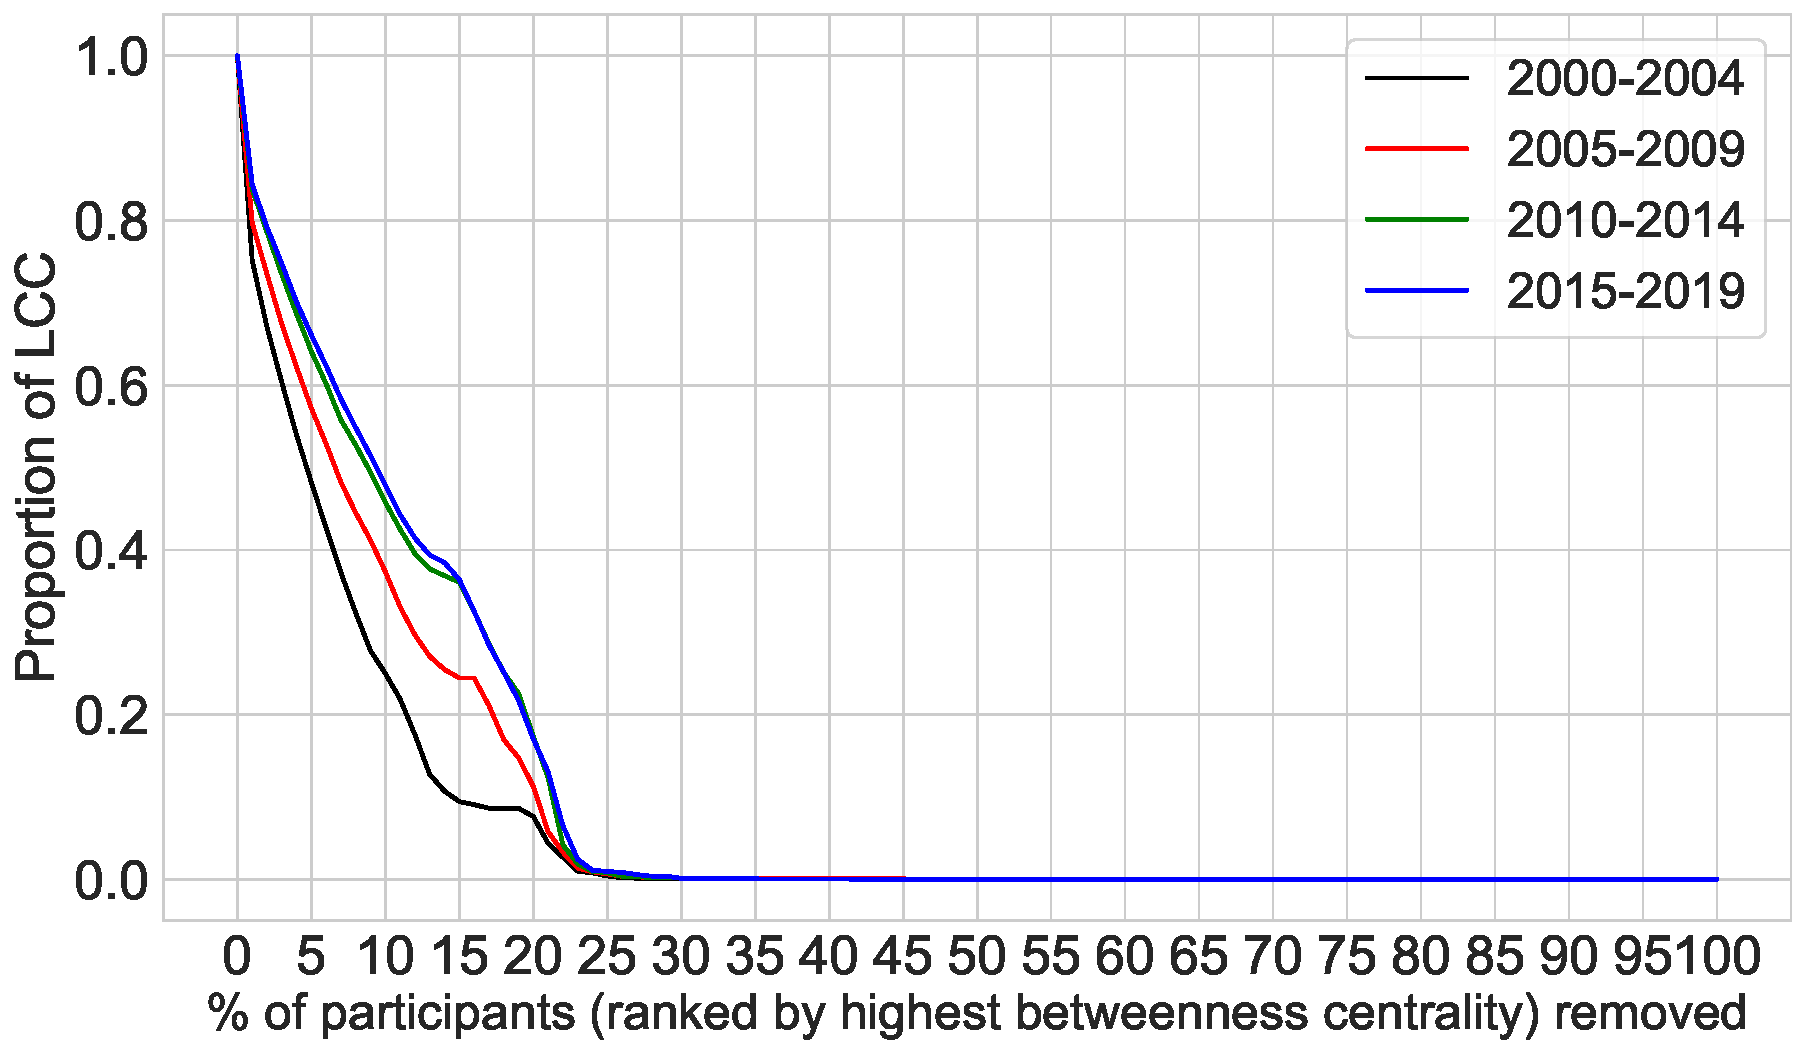
\includegraphics[width=\figureWidthOneColumn]{figures-prev/icwsm-2022/lcc_proportion_granular_yearly.pdf}
  \caption{
    Impact of removing participants by their influence on the size
    of the LCC.
  }
  \label{fig:purge_nodes_largest_connected_component_number_components}
\end{figure}

% - - - - - - - - - - - - - - - - - - - - - - - - - - - - - - - - - - - - - - - - - - - - - - - - -
\subsubsection{Behaviour of Influential Participants}
\label{subsec:influencer_behaviour}

% ICWSM 2022 paper Section 3.2

We now characterise the behaviour of the most influential participants, as
measured by betweenness centrality (\S\ref{subsec:measuring_influence}), in
terms of the volume of emails they send, the length of time they ate active
within the community, and the topics discussed. 

%..................................................................................................
\pb{Email volume:}
Figure~\ref{fig:emailcount_top_percentile} shows that each participant in
the top 10\% most influential participants sends on average around
0.05\%-0.08\% of total emails in a given period.  Collectively, the top
10\% most influential participants account for 43.75\%, on average, of the
total number of emails sent, a substantially larger proportion than the
other participants.

This ratio seems broadly stable over yet the overall number of emails sent
increases up to 2010 and remains roughly constant from then onward.  Along
with the results from \S\ref{subsec:measuring_influence}, this shows a
worrying, if slowly improving, dependence of the IETF on a small number of
highly influential participants.

\begin{figure}
  \centering
  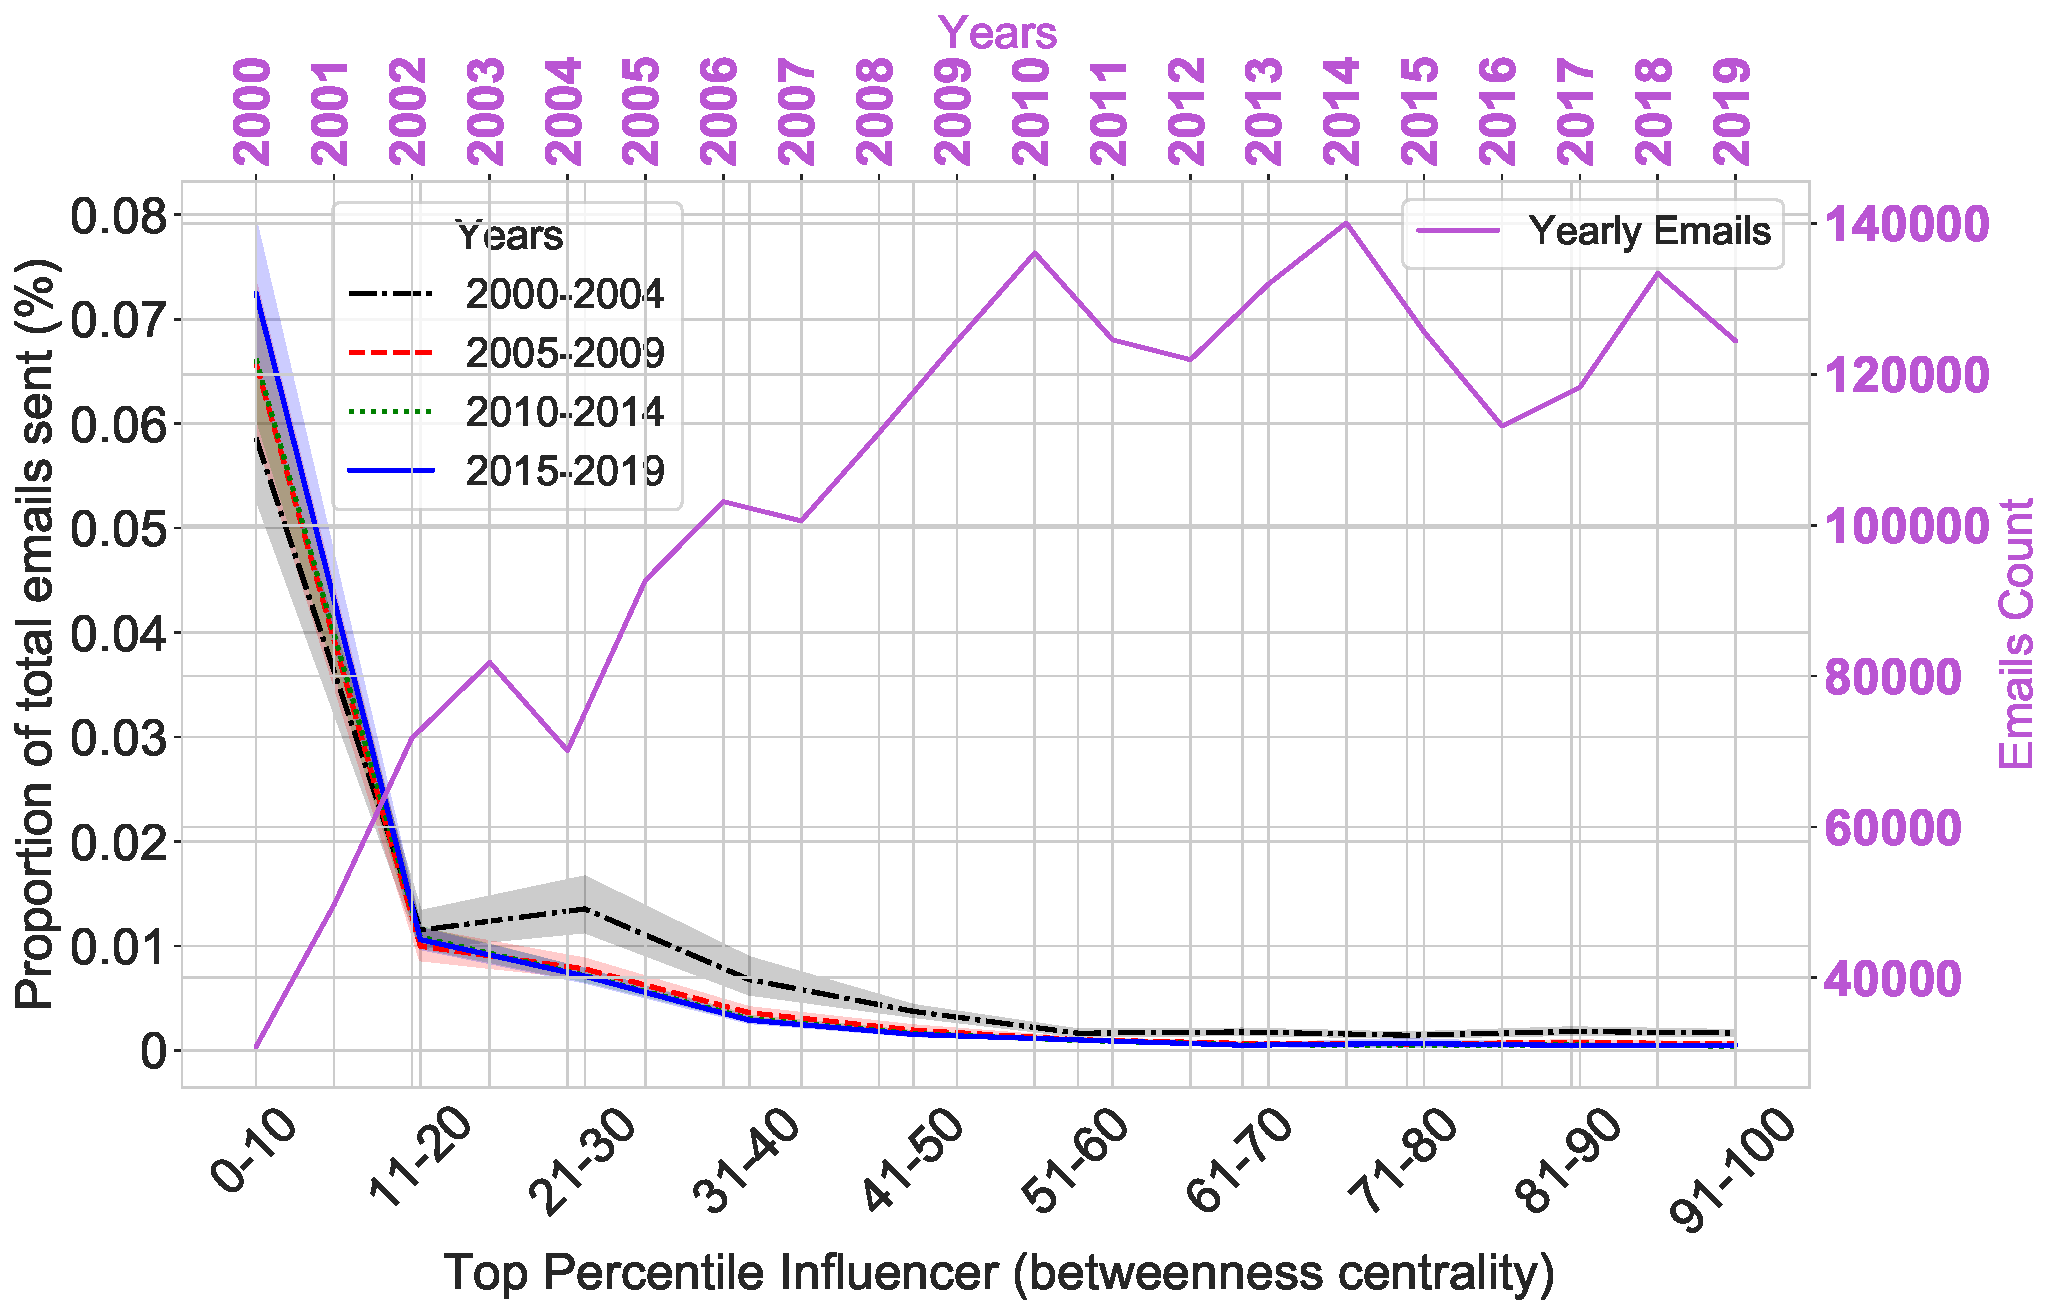
\includegraphics[width=\figureWidthOneColumn]{figures-prev/icwsm-2022/lineplot_proportion_emailscount_top_percentile.pdf}
  \caption{
    Proportion of emails sent (\%) by participants in each period (with
    95\% confidence interval) according to their betweenness-centrality
    percentile (x-axis).  Y2-axis (purple) shows yearly count of emails.
  }
  \label{fig:emailcount_top_percentile}
\end{figure}

%..................................................................................................
\pb{Cross-area review:} 
In addition to sending more emails, we test if influential participants
engage with different parts of the community more often than do typical
participants. That is, we measure if influential participants are more
likely to make contributions to working groups in multiple IETF Areas.

Figure~\ref{fig:areas_participation_top_percentile} shows the mean number
of areas where participants in the IETF are active (based on the set of
mailing lists they sent do). We see that more influential participants
engage in more areas of the IETF, on average, than do less influential
participants: not only do influential participants send more email, they
send email to working groups in more areas of the IETF. This indicates
that influential participants benefit the IETF in enabling cross-area
discussion and review, and can bridge administrative divisions.

It can also be seen that cross-area engagement has improved over time,
with participants as a whole sending email to groups in more areas over
tine. This shows that the IETF community as a whole is discussing more 
broadly than it used to, perhaps further indication of the increasing
complexity of the standards development and widespread concern about
feature interactions.

\begin{figure}
  \centering
  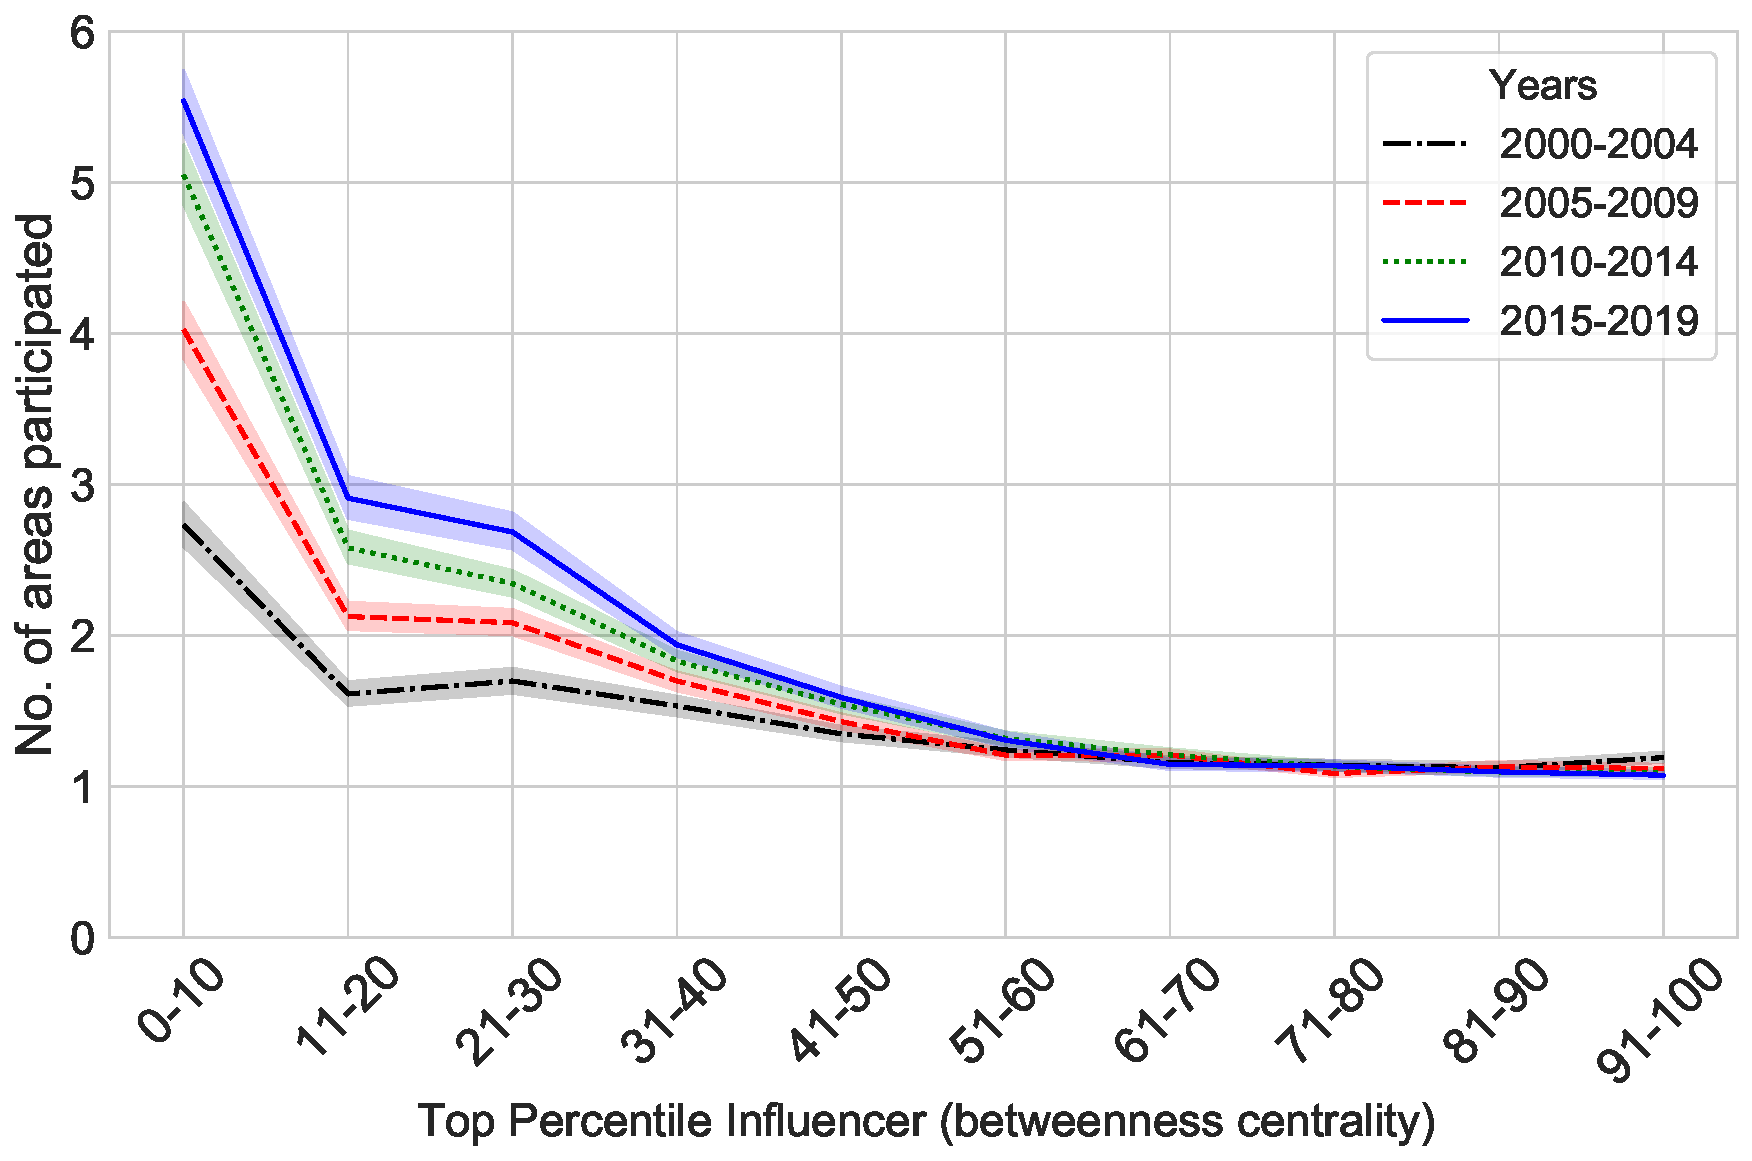
\includegraphics[width=\figureWidthOneColumn]{figures-prev/icwsm-2022/lineplot_avg_areas_top_percentile.pdf}
  \caption{
    Mean number of areas participated in (with 95\% confidence interval)
    according to their betweenness-centrality percentile in the x-axis,
    ranked from top (0-10) to bottom percentile (91-100).
  }
  \label{fig:areas_participation_top_percentile}
\end{figure}

%..................................................................................................
\pb{Participation duration:}
We next consider how long participants remain associated with the IETF,
measured as the time between sending their first and last emails to one of
the mailing lists.

Figure~\ref{fig:age_top_percentile} shows the mean participation duration
distribution for participants, ranked by influence. Participation duration
increases over time, with the most influential participants typically being
those who have been active for longer. While this might be expected, it
might be a good sign for the IETF community in that it implies that the
most influential participants are also the most experienced.
The short participation duration of the less influential participants
matches the participant churn discussed in Figure \ref{fig:author_new}
in \S\ref{sec:trends-demographics:affiliation}.

\begin{figure}
  \centering
  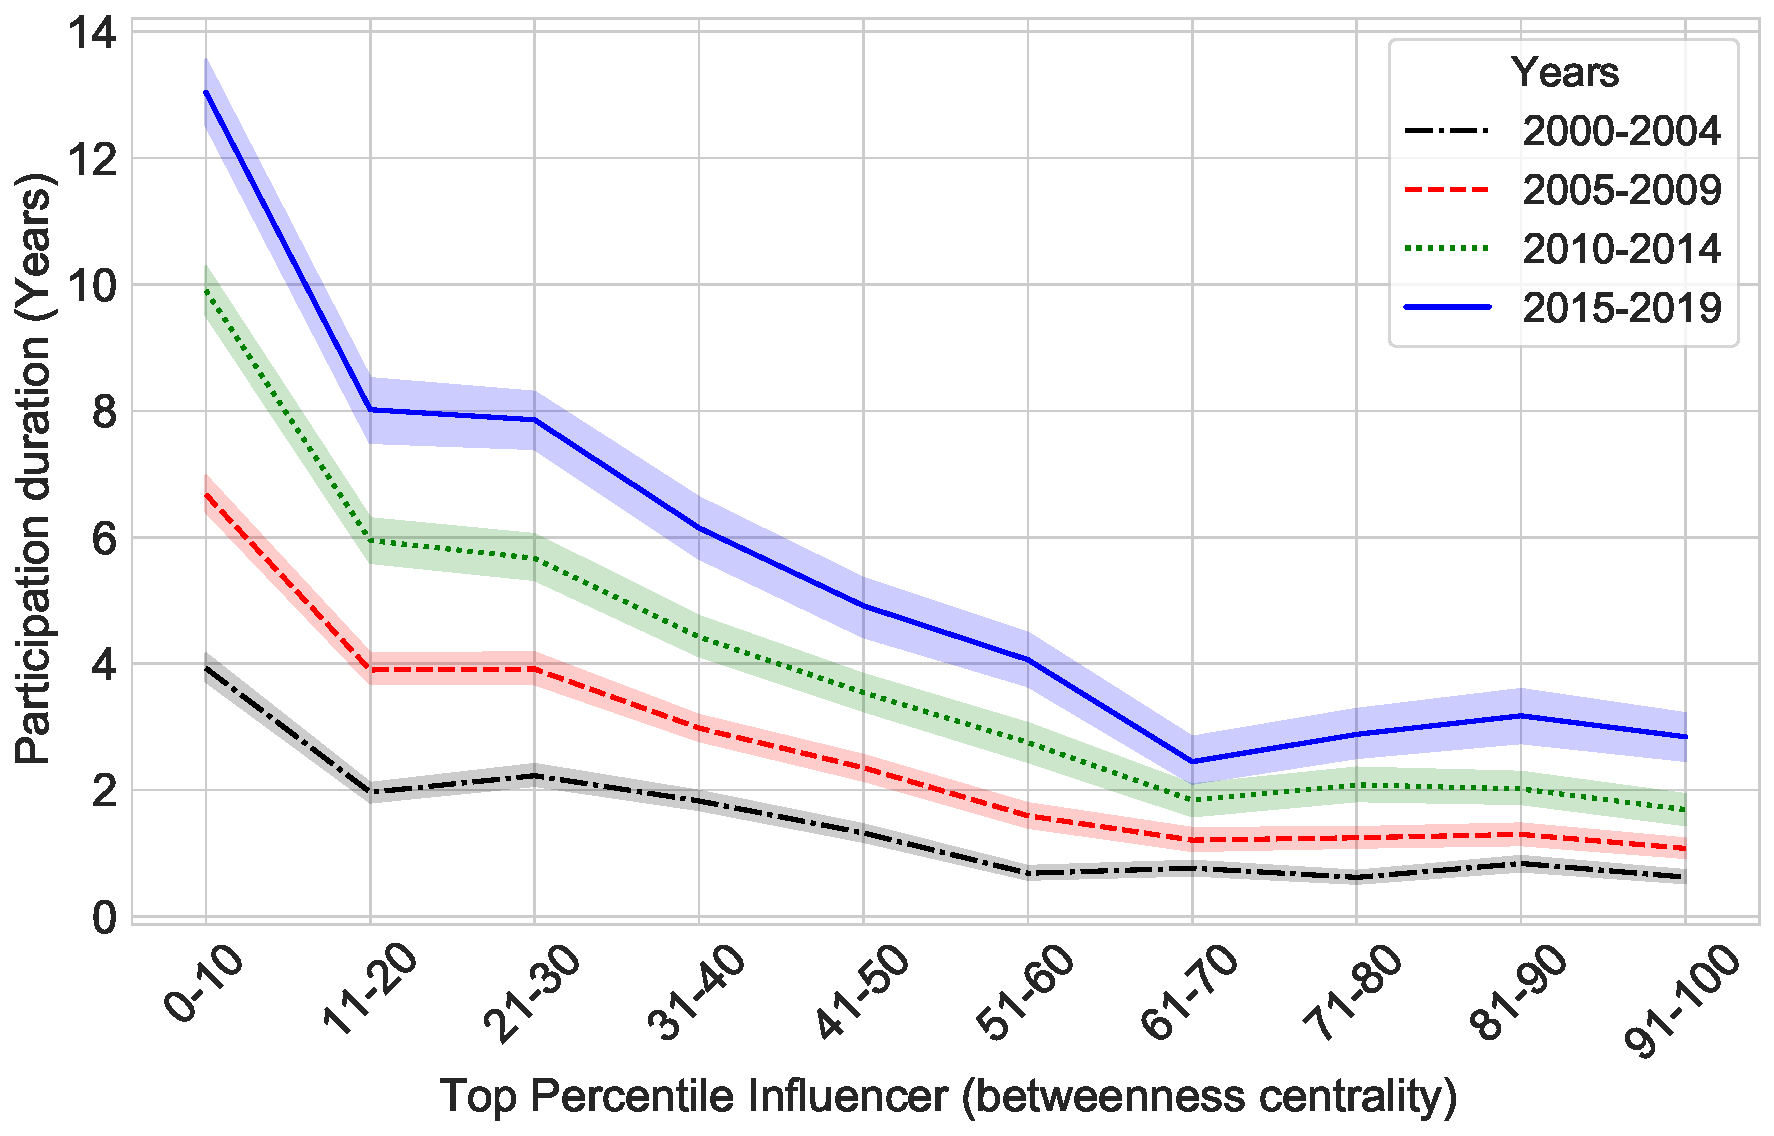
\includegraphics[width=\figureWidthOneColumn]{figures-prev/icwsm-2022/lineplot_age_top_percentile.pdf}
  \caption{
    Mean participation duration (with 95\% confidence interval) according
    to their betweenness-centrality percentile in the x-axis, ranked from
    top (0-10) to bottom percentile (91-100).
  }
  \label{fig:age_top_percentile}
\end{figure}

We further consider whether participants who become influential, remain
influential. Figure \ref{fig:heatmap_top10_overlap} shows what proportion
of the top 10\% influential participants in any given year (\emph{y-axis})
was also among the top 10\% influential participants in any other year
(\emph{x-axis}). This shows that a significant majority of participants
that become influential, continue to be influential for a number of years:
the top 10\% are influential for at least 6-7 years on average.

\begin{figure}
  \centering
  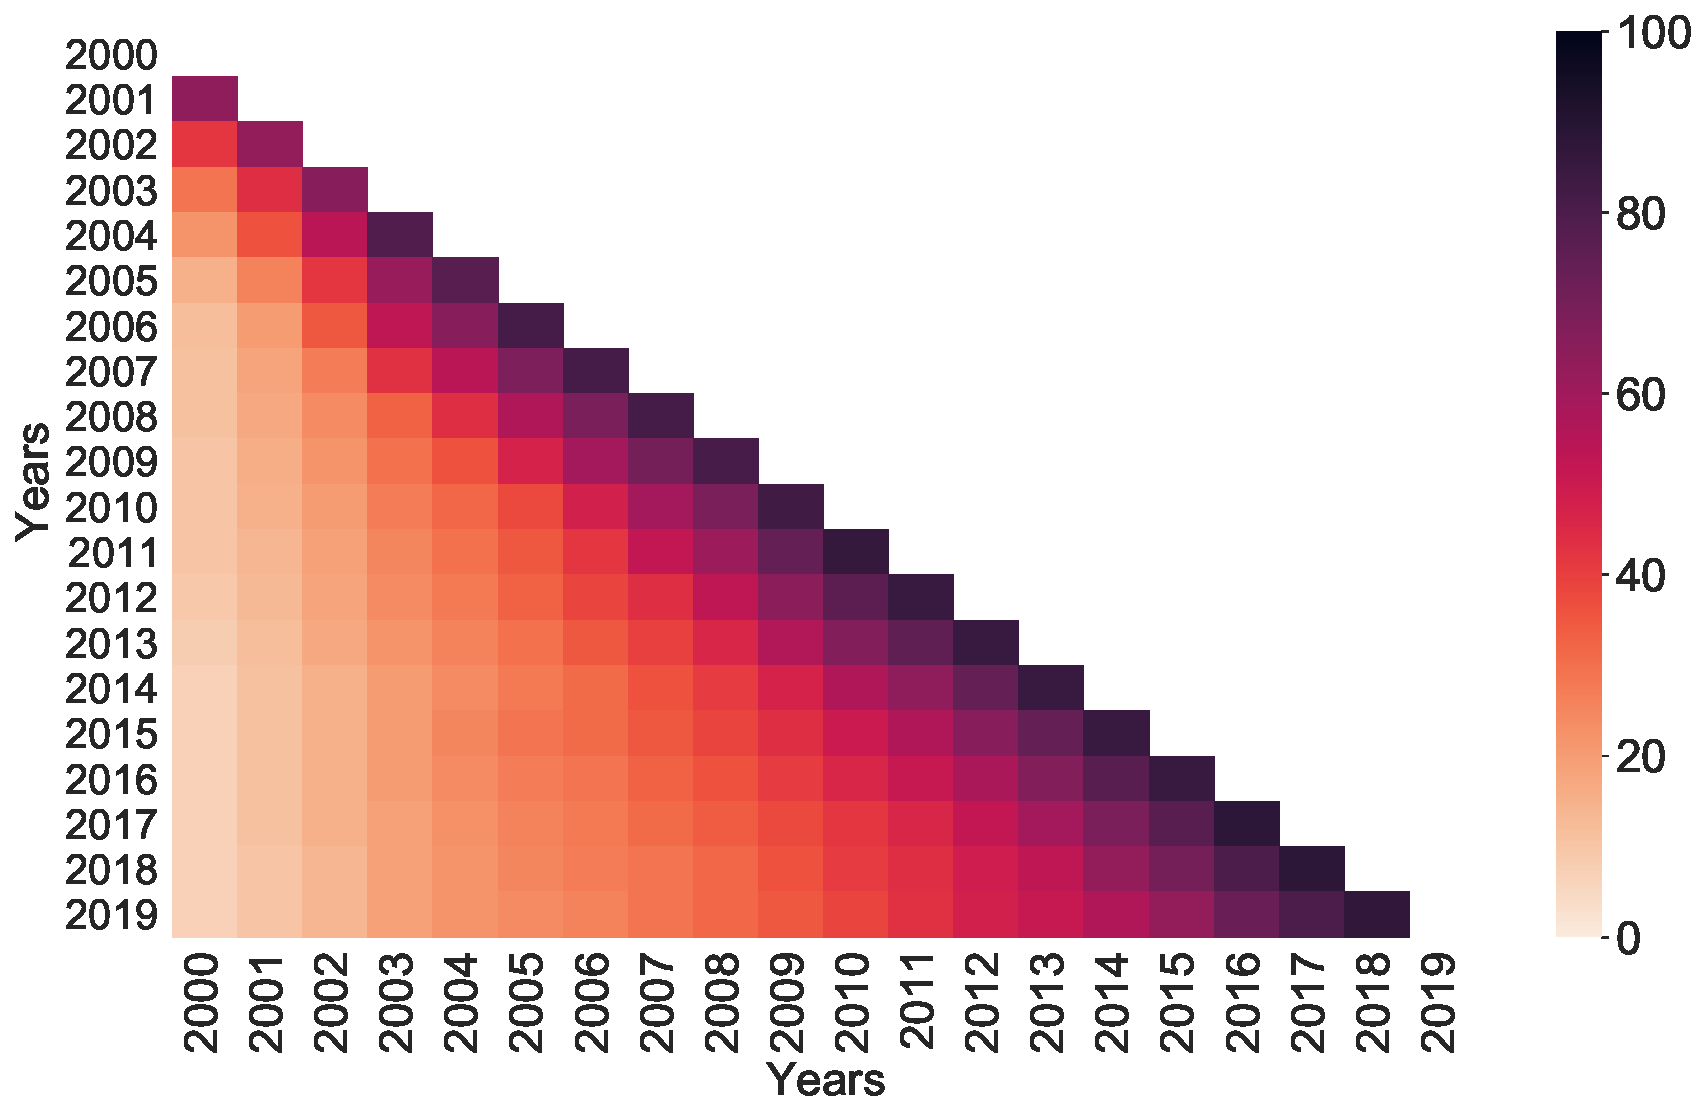
\includegraphics[width=\figureWidthOneColumn]{figures-prev/icwsm-2022/heatmap_top10_percent_overlap.pdf}
  \caption{
    Yearly overlap (\%) of top 10\% influencers.
  }
  \label{fig:heatmap_top10_overlap}
\end{figure}

Finally, Figure \ref{fig:rate_new_influential_participants} shows that
breaking into the top 10\% of influencers requires an increasing number of
years of participation. This may be beneficial, showing that the IETF is
maturing and is capable of retaining influential and experienced
participants, but it may also point to an increasingly ossified structure
that is not welcoming to newcomers.

\begin{figure}
  \centering
  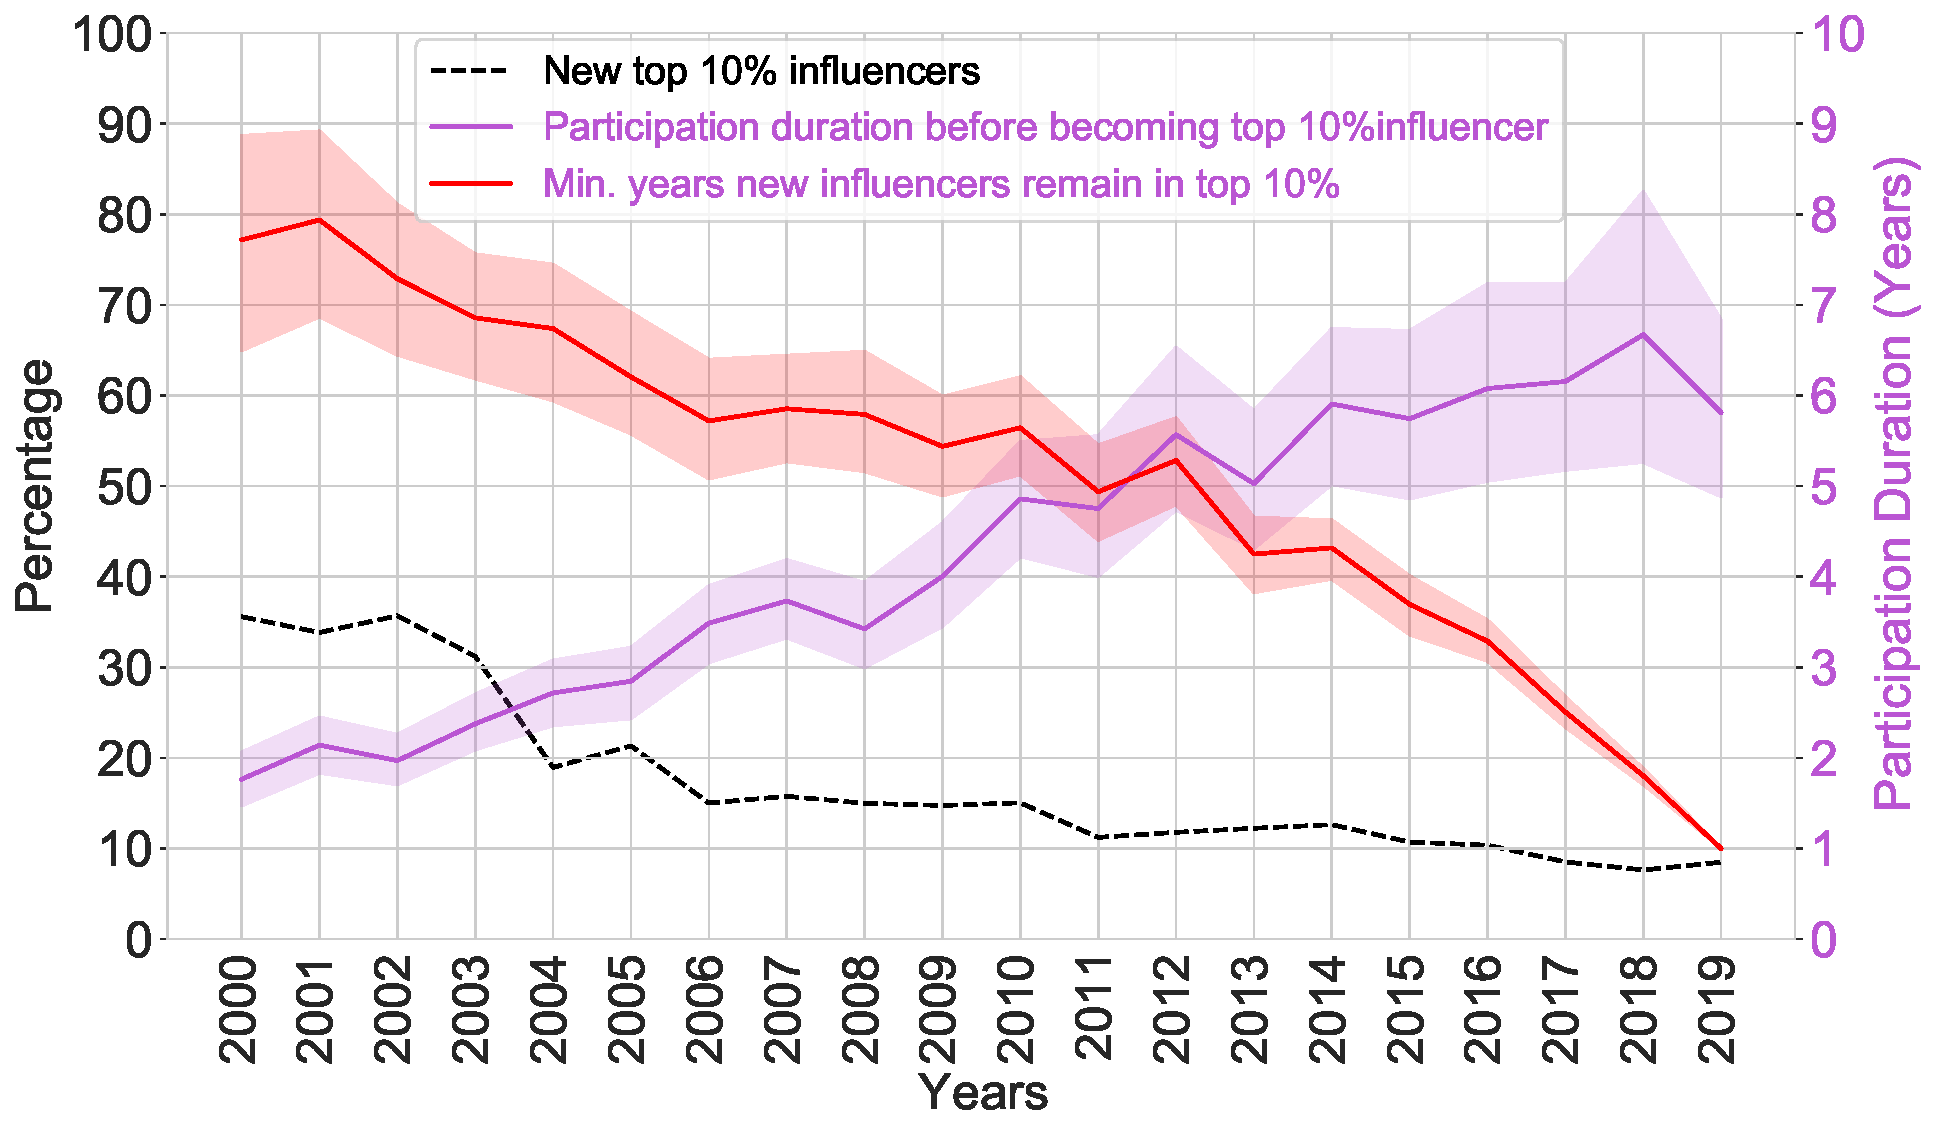
\includegraphics[width=\figureWidthOneColumn]{figures-prev/icwsm-2022/new_influencers_top10_age_longevityInTop10.pdf}
  \caption{
    Percentage of new influential participants breaking into top 10\%
    influencers (black); the average years of participation before entering
    top 10\% (purple); and minimum \#  years new influencers remain in top
    10\% (with 95\% confidence intervals).
  }
  \label{fig:rate_new_influential_participants}
\end{figure}

%..................................................................................................
\pb{Topics of Discussion:} 
The topics discussed on working group mailing lists are a good indicator
of the focus of technical work, and it might be expected that influential
participants will set the direction of that work. To explore this, we use
the Latent Dirichlet Allocation (LDA) \cite{blei2003latent,hoffman2010online}
model from \texttt{gensim} \cite{rehurek_lrec} to induce 100 topics on the
entire set of email texts. 

Each topic is a distribution over words. For example, a \emph{security}
topic might have high probability for \emph{cypher}, \emph{rsa},
\emph{auth}, and related words. We can also use the model to obtain a
vector for any input text as a sparse distribution over all topics, e.g.,
finding that a text is comprised of 30\% security and 70\% video streaming
topics. With this, we generate a vector for each participant in a given
time period by concatenating all messages sent by that participant in the
period and feeding it into the LDA model. The result can be loosely
interpreted as a distribution of topics on which each participant works.

Manual inspection of the induced topics reveals some interesting trends. We
find that topics related to \emph{routing} and \emph{email} protocols are
seeing a steady decline in popularity, while topics like \emph{streaming}
and \emph{cryptography} are becoming more prominent. This reflects wider
trends in standardisation, as these efforts have adjusted to the public's
increased awareness of privacy, especially in light of the Edward Snowden
leaks \cite{RFC7258,RFC9446}. We also find that as videoconferencing became
increasingly popular, so did the WebRTC protocol that frequently underpins
them.

We next measure the topical diversity of a participant by observing the
entropy of their topic vector, their \emph{topic entropy}, defined as
follows:
\begin{equation}
  \eta = - \sum_{i=1}^{|T|} p_i \log p_i \nonumber
\end{equation}
where $T = [p_1, ..., p_N]$ is a topic vector, which defines a probability
distribution over $N$ topics, each $p_i$ is a probability of the $i$-th
topic and $\sum_i p_i = 1$.

Figure \ref{fig:topic_diversity} shows topic entropy distributions of
participants in different time periods and influence percentiles. While we
initially experimented with measuring diversity by simply counting the
number of topics that account for the majority ($ \geq 95\% $) of a
participant's topic distribution probability mass, we found that most
participants engage in a relatively small number of topics, regardless of
influence. However, after measuring diversity using entropy, we identify
that the activity of the more influential participants tends to be more
evenly spread across the topics they participate in\footnote{An example
with 3 topics: a distribution of $[0.8, 0.1, 0.1]$ is less evenly spread
than $[0.3, 0.4, 0.3]$.}. This difference becomes more pronounced over
time, implying that increased topic entropy (i.e.,~more evenly participating
in different topics) is an increasingly salient property of influencers.
This is aligned with our earlier findings on cross-area review, showing the
growing number of areas in which influencers participate.


\begin{figure}
  \centering
  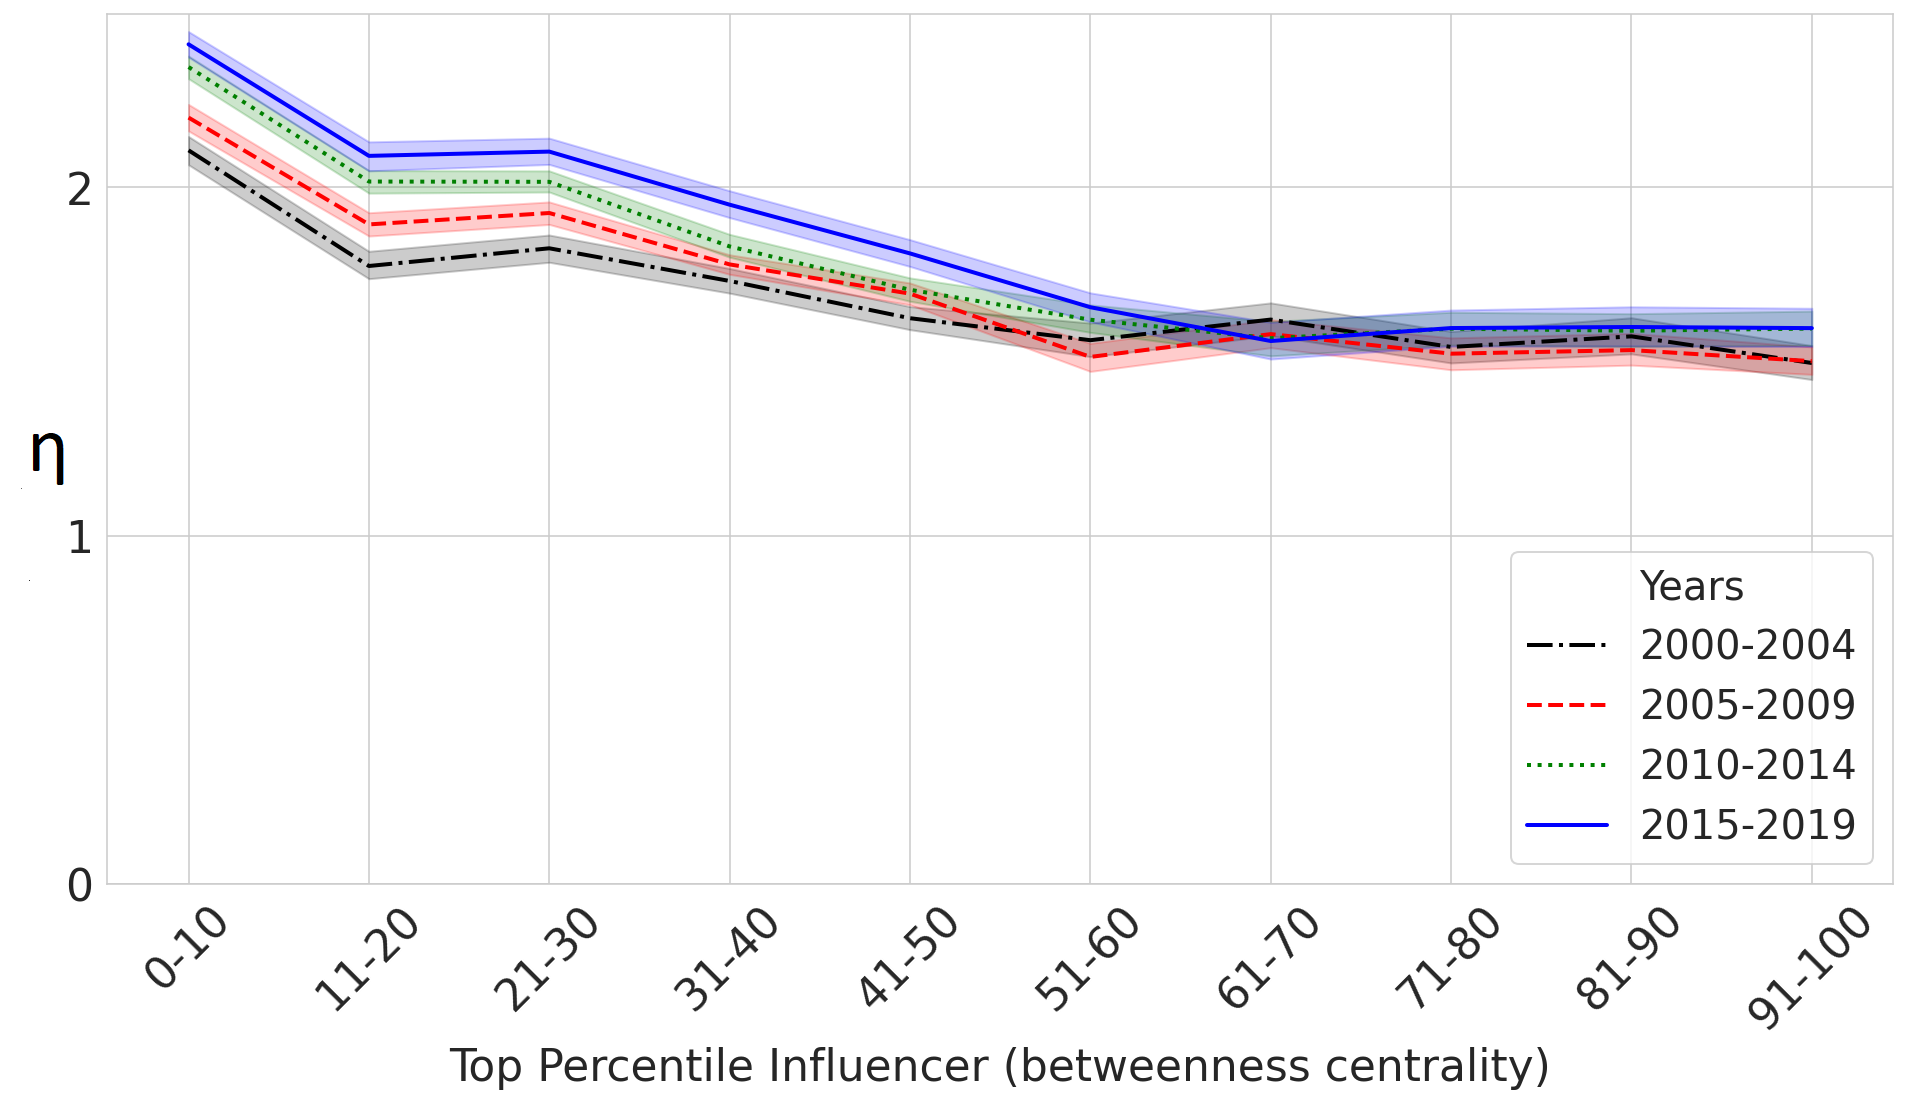
\includegraphics[width=\figureWidthOneColumn]{figures-prev/icwsm-2022/topic-div.png}
  \caption{
    Mean topic entropy (with 95\% confidence interval) according to their
    betweenness-centrality percentile in the x-axis, ranked from top (0-10)
    to bottom percentile (91-100).
  }
  \label{fig:topic_diversity}
\end{figure}


% - - - - - - - - - - - - - - - - - - - - - - - - - - - - - - - - - - - - - - - - - - - - - - - - -
\subsubsection{Impact of Influential Participants}
\label{subsec:impact_influence}

% ICWSM 2022 paper Section 3.3

While the top participants are defined by the betweenness centrality metric
(\S\ref{subsec:measuring_influence}) as being influential within the IETF
mailing lists, it is unclear how this influence translates into document
authorship and leadership roles within the IETF.  We explore these aspects
of influence in the following.

%..................................................................................................
\pb{Document authorship:}
The output of the IETF is technical standards and other documents published
in the RFC series. RFCs are developed by working groups from a sequence of
Internet-drafts, with individuals acting as named authors. Having identified
the most influential participants in the mailing list community, we can
determine whether or not these same participants are also the most active
authors.

Figure~\ref{fig:drafts_initiation_top_percentile} shows the distribution of
the proportion of documents authored by mailing list participants, sorted
by their influence rank. We observe that:
(i) influential participants in the email graph, i.e., those ranked top in
betweenness centrality, tend to write more drafts than do participants with
lower centrality; and
(ii) the number of drafts per participant is increasing over time for all
participants.
For example, during 2010-2019, each participant in the top 10 percentile,
authored 0.125\% to 0.175\% of the total number of drafts in that period.
We find that 32\%-42\% of the total drafts, in different years during this
period, were authored by the top 10\% most influential mailing list
participants.

\begin{figure}
  \centering
  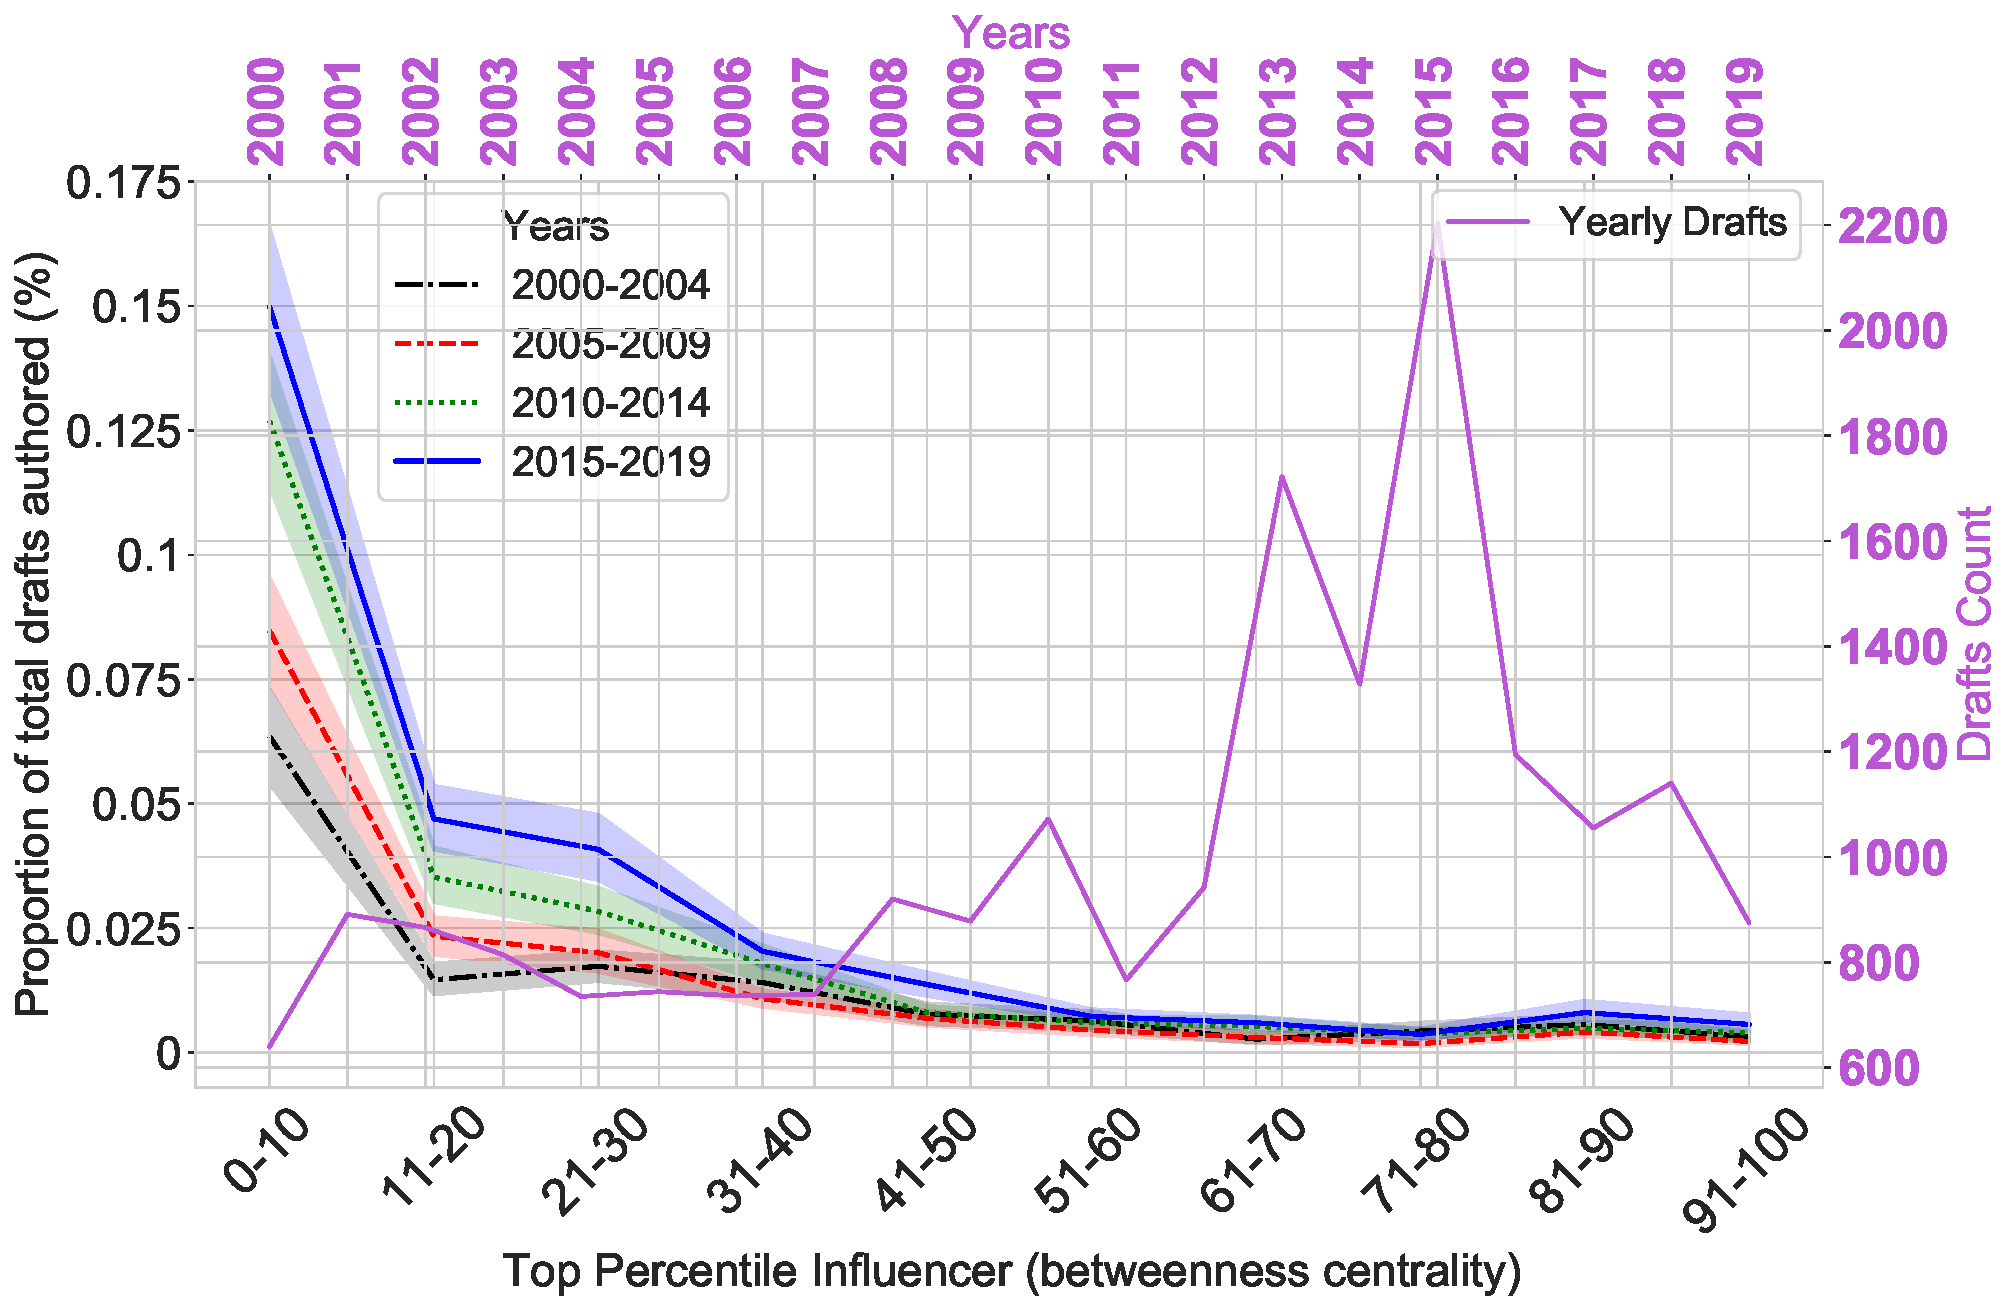
\includegraphics[width=\figureWidthOneColumn]{figures-prev/icwsm-2022/documents_proportion_published_top_percentile.pdf}
  \caption{
    Average drafts authored (with 95\% confidence interval) according to
    their betweenness-centrality percentile in the x-axis, ranked from top
    (0-10) to bottom percentile (91-100).  Right-y axis (purple) shows
    yearly drafts per year.
  }
  \label{fig:drafts_initiation_top_percentile}
\end{figure}

%..................................................................................................
\pb{Document co-authorship and correlation with the email graph:}
Figure~\ref{fig:drafts_initiation_top_percentile} showed that influential
participants on the mailing lists tend to author more drafts than others.
We next ask if they are also influencers in the draft co-authorship graph.

To do this, we create a draft co-authorship graph where each author is a
node, and draft co-authorship is an edge. We then measure influence with
betweenness centrality of the authors in each time period.
Table~\ref{tbl:correlation_sprmn} compares the top 20\% of influencers of
the mailing lists with those of the co-authorship graph.  We find a
significant overlap between both groups, ranging from 48.2\% to 67.2\%.
There is a significant ($p < 0.05$) positive correlation between the
rankings of the overlapping members of each community: participants that
are influential in the mailing lists are also likely to be influential in
draft authorship.

\begin{table}
  \small 
  \begin{tabular}{llllll}
    \toprule
    \multicolumn{6}{c}{Top 20\% draft authors \& all email participants}\\ \midrule
                    
    Years   & \multicolumn{2}{c}{Sub-Network Size} & Overlap  & \multicolumn{2}{c}{Spearman's $r_{s}$} \\ \cline{2-3}  \cline{5-6}
        &   Co-author & Email  &  &   $r_{s}$   & $p$-value \\ \midrule
        
    2000-04   &   398 &   1390 &   48.24\%  &  .323 &   4.75e-06 \\
    2005-09   &   427 &   1662 &   67.21\% &   .332   &   7.39e-09    \\
    2010-14   &   728 &   1639 &   63.05\% &   .299   &   5.73e-11  \\
    2015-19   &   915 &   1370 &   55.85\%  &   .337   &   4.13e-15  \\ %\hline
       
    \bottomrule
  \end{tabular}
  \caption{
    Overlap in the co-author and email graph.
  }
  \label{tbl:correlation_sprmn}
\end{table}

We also look at the top 20\% participants from the co-authorship network
who are \emph{not} part of the top 20\% influencers in the email network in
Figure \ref{fig:non_overlapping_coauthornetwork_authors_emailnetwork}.
We observe that some prolific authors are \emph{not} engaged
in the email discussion: 40\%-50\% of non-overlapping authors are ranked
between 20th to 40th percentile of influence in the email network. These
non-overlapping authors are typically more junior with respect to their
participation duration.

\begin{figure}
  \centering
  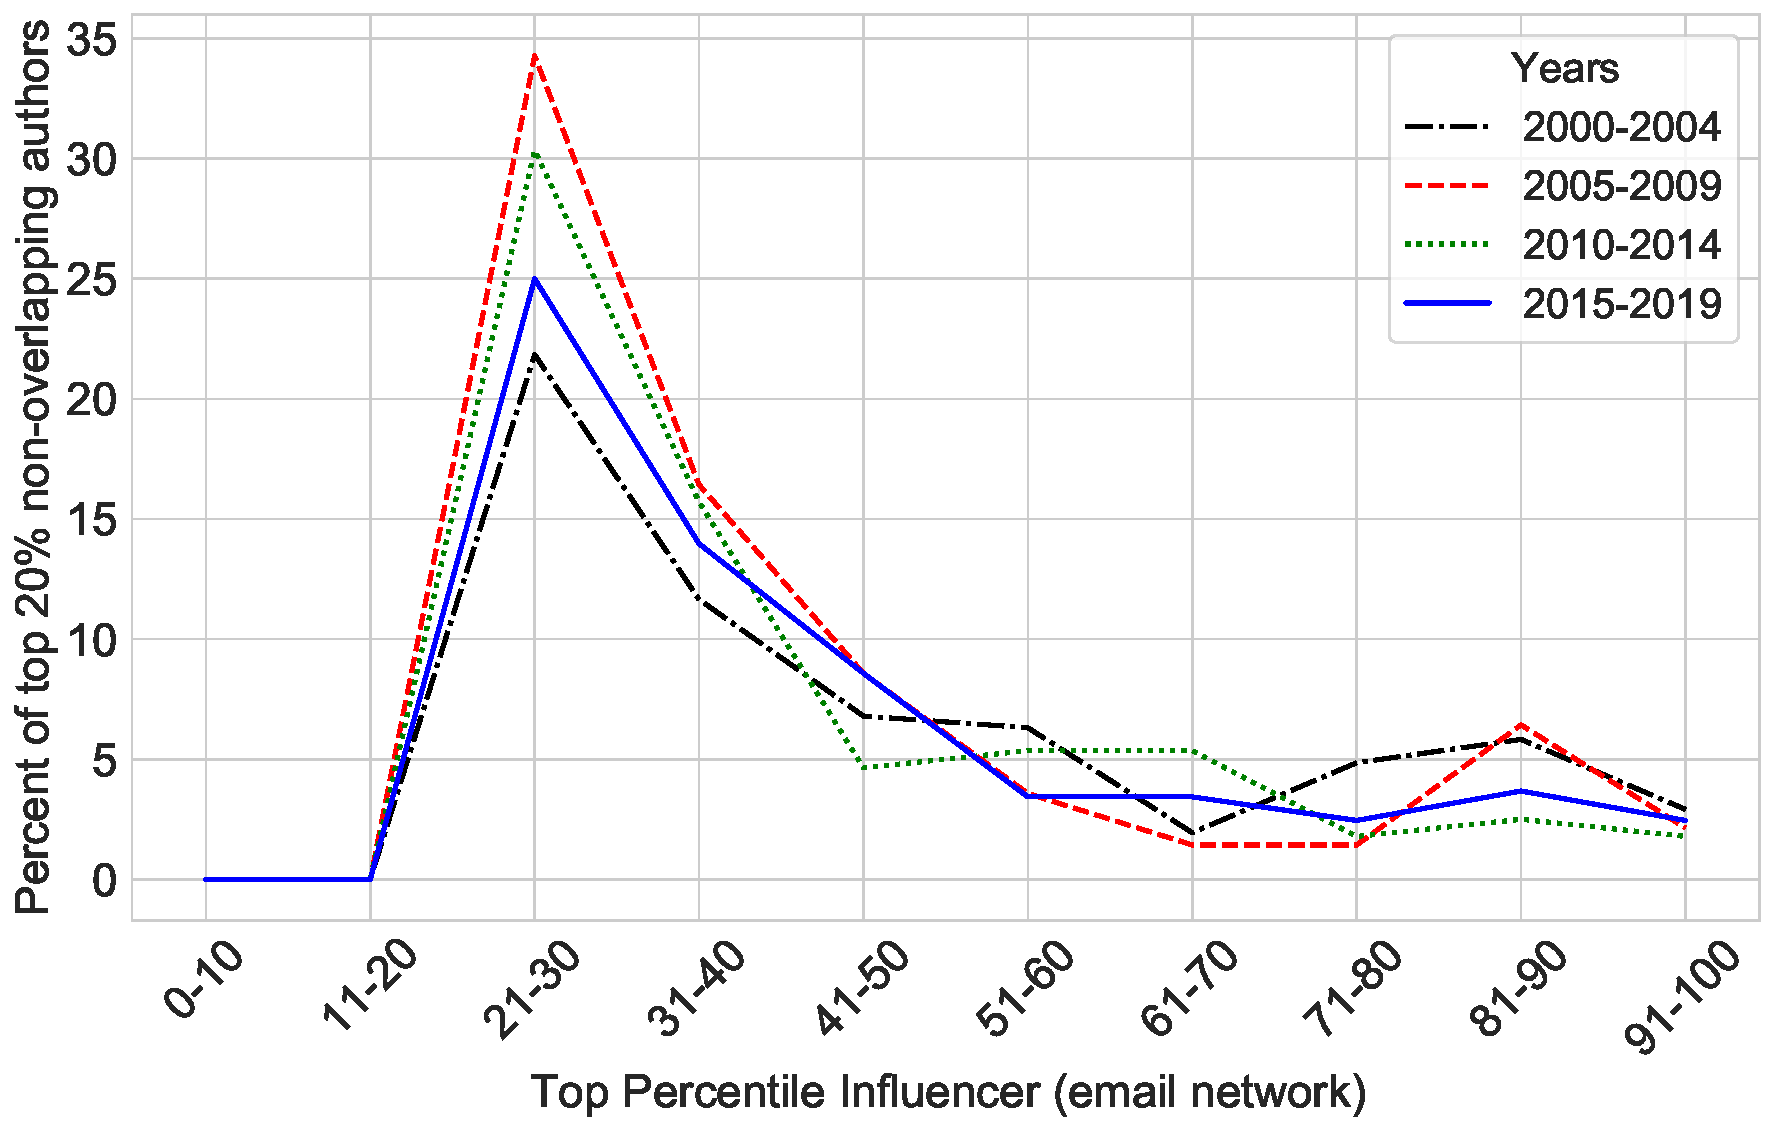
\includegraphics[width=\figureWidthOneColumn]{figures-prev/icwsm-2022/coauthor_affiliation_network/lineplot_non_overlapping_authors_emailnetwork_percentile.pdf}
  \caption{
    Percentage of Top 20\% authors that are not 20\% influencers according
    to their betweenness-centrality (email graph) percentile in the x-axis,
    ranked from  top (0-10) to bottom percentile (91-100).
  }
  \label{fig:non_overlapping_coauthornetwork_authors_emailnetwork}
\end{figure}

%..................................................................................................
\pb{Influencers and leadership roles:} 
Working group chairs are selected from the community, so we might expect
those selected to be influential in the community.
Figure~\ref{fig:wg_chair_before_after} shows that this is indeed the case:
87.5\% of working group chairs are in the top 20\% of mailing list
influencers and 67.4\% are in the top 20\% of document authors in the year
before they became chairs. This also shows the impact of taking up a
leadership role: influence in both the mailing list and authorship
communities grows in the year after participants become a working group
chair for the first time. 

\begin{figure}
  \centering
  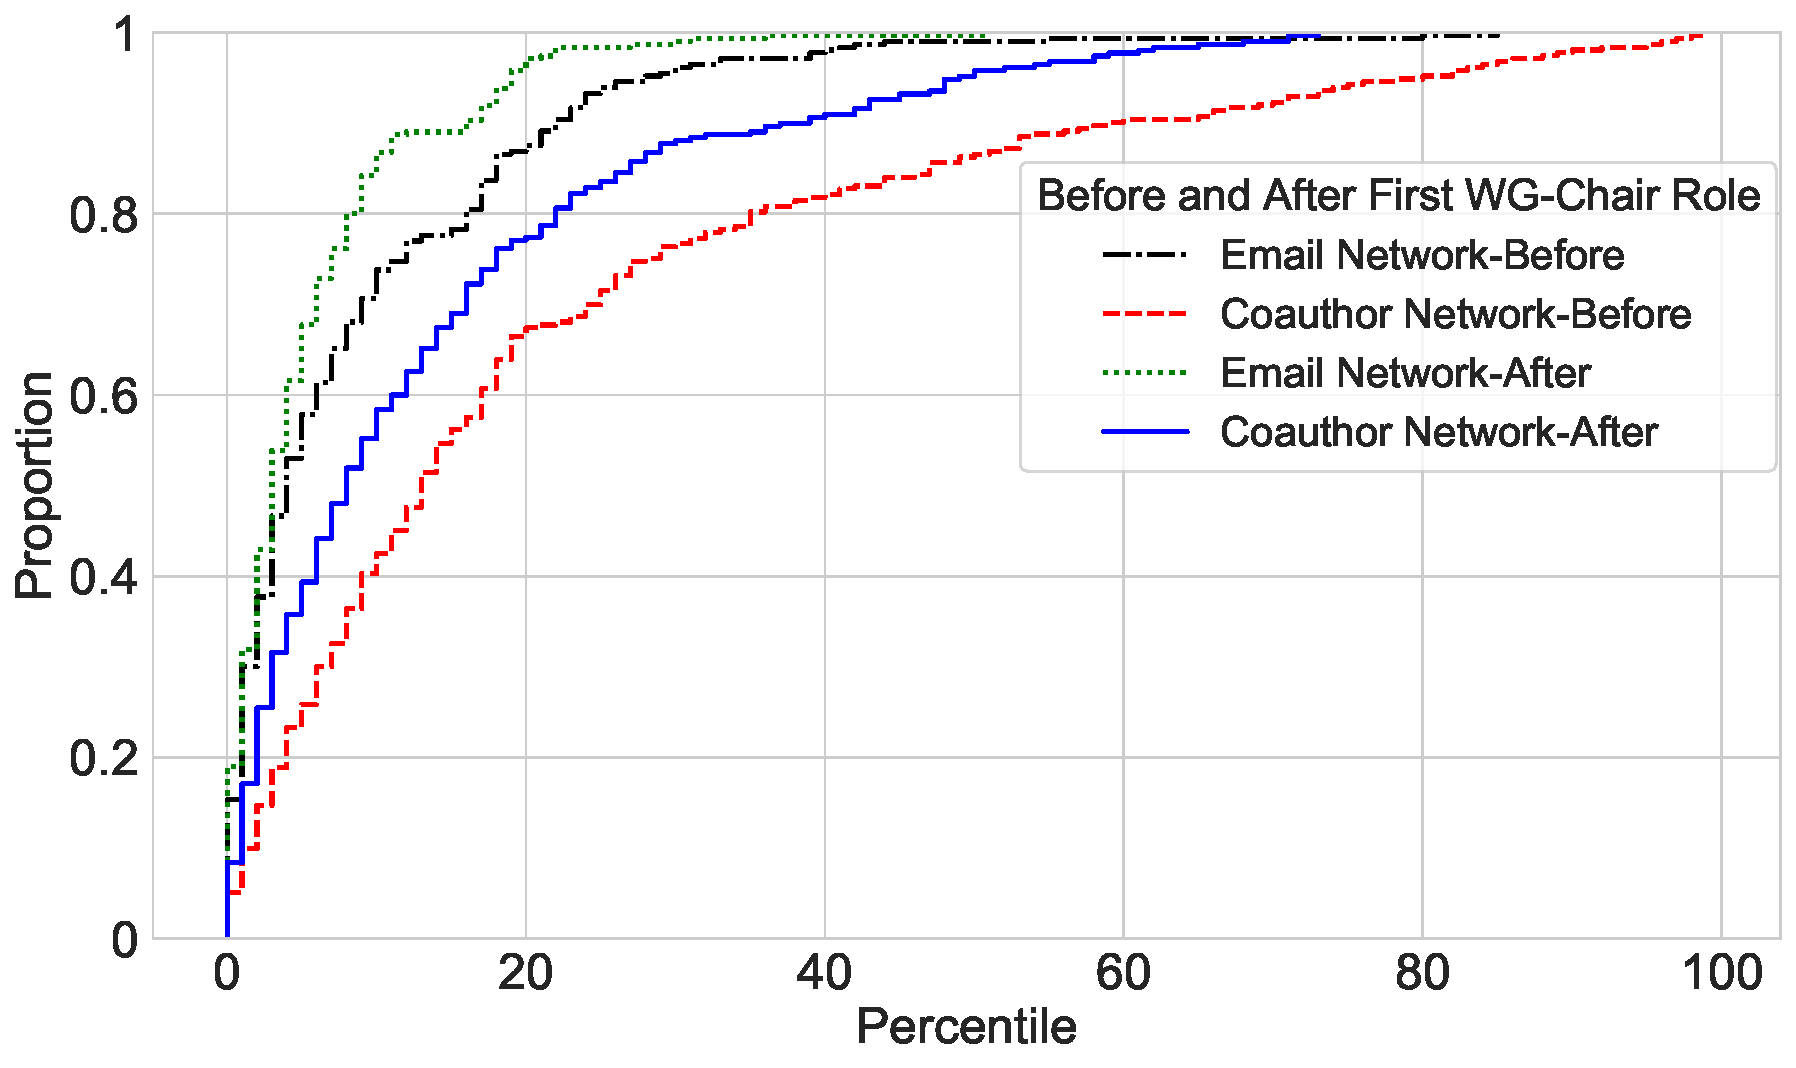
\includegraphics[width=\figureWidthOneColumn]{figures-prev/icwsm-2022/WG_chair_percentile_CDF_before_after.pdf}
  \caption{
    CDF of the percentile of betweenness-centrality of WG chairs in the
    email and co-authorship graph, one year before and after becoming
    chairs.
  }
  \label{fig:wg_chair_before_after}
\end{figure}

%..................................................................................................
\pb{Influence of organisations:}
While participants in the IETF are expected to contribute as individuals,
they are usually affiliated with an organisation.  To study the potential
influence of those organisations, for each draft we obtain the authors'
affiliations from the Datatracker. If this is not available, we use the
domain name of the authors' email addresses, which we map to the relevant
organisation (e.g., \texttt{@cisco.com} maps to Cisco). For generic email
addresses, such as \texttt{@gmail.com}, we use the participant name if no
affiliation is available.

Figure \ref{fig:coauthor_affiliation_network2019_otheryears} shows the ten
most frequent affiliated organisations of the top 20\% of draft authors in
the period 2015-2019, and the number of authors affiliated with these
organisations in  each  period.  While the dominance of Cisco is clear,
other organisations, such as Huawei, have gained a larger presence over
time.  In general, a small number of organisations employ a significant
fraction of the influential participants in the standards process. If we
look at the period 2015-2019, for example, out of the 915 authors ranked in
the top 20\% of most influential authors, 342 belong to the ten most
frequently affiliated organisations, and nearly 253 are from Cisco, Huawei,
Ericsson, or Juniper alone.

\begin{figure}
  \centering
  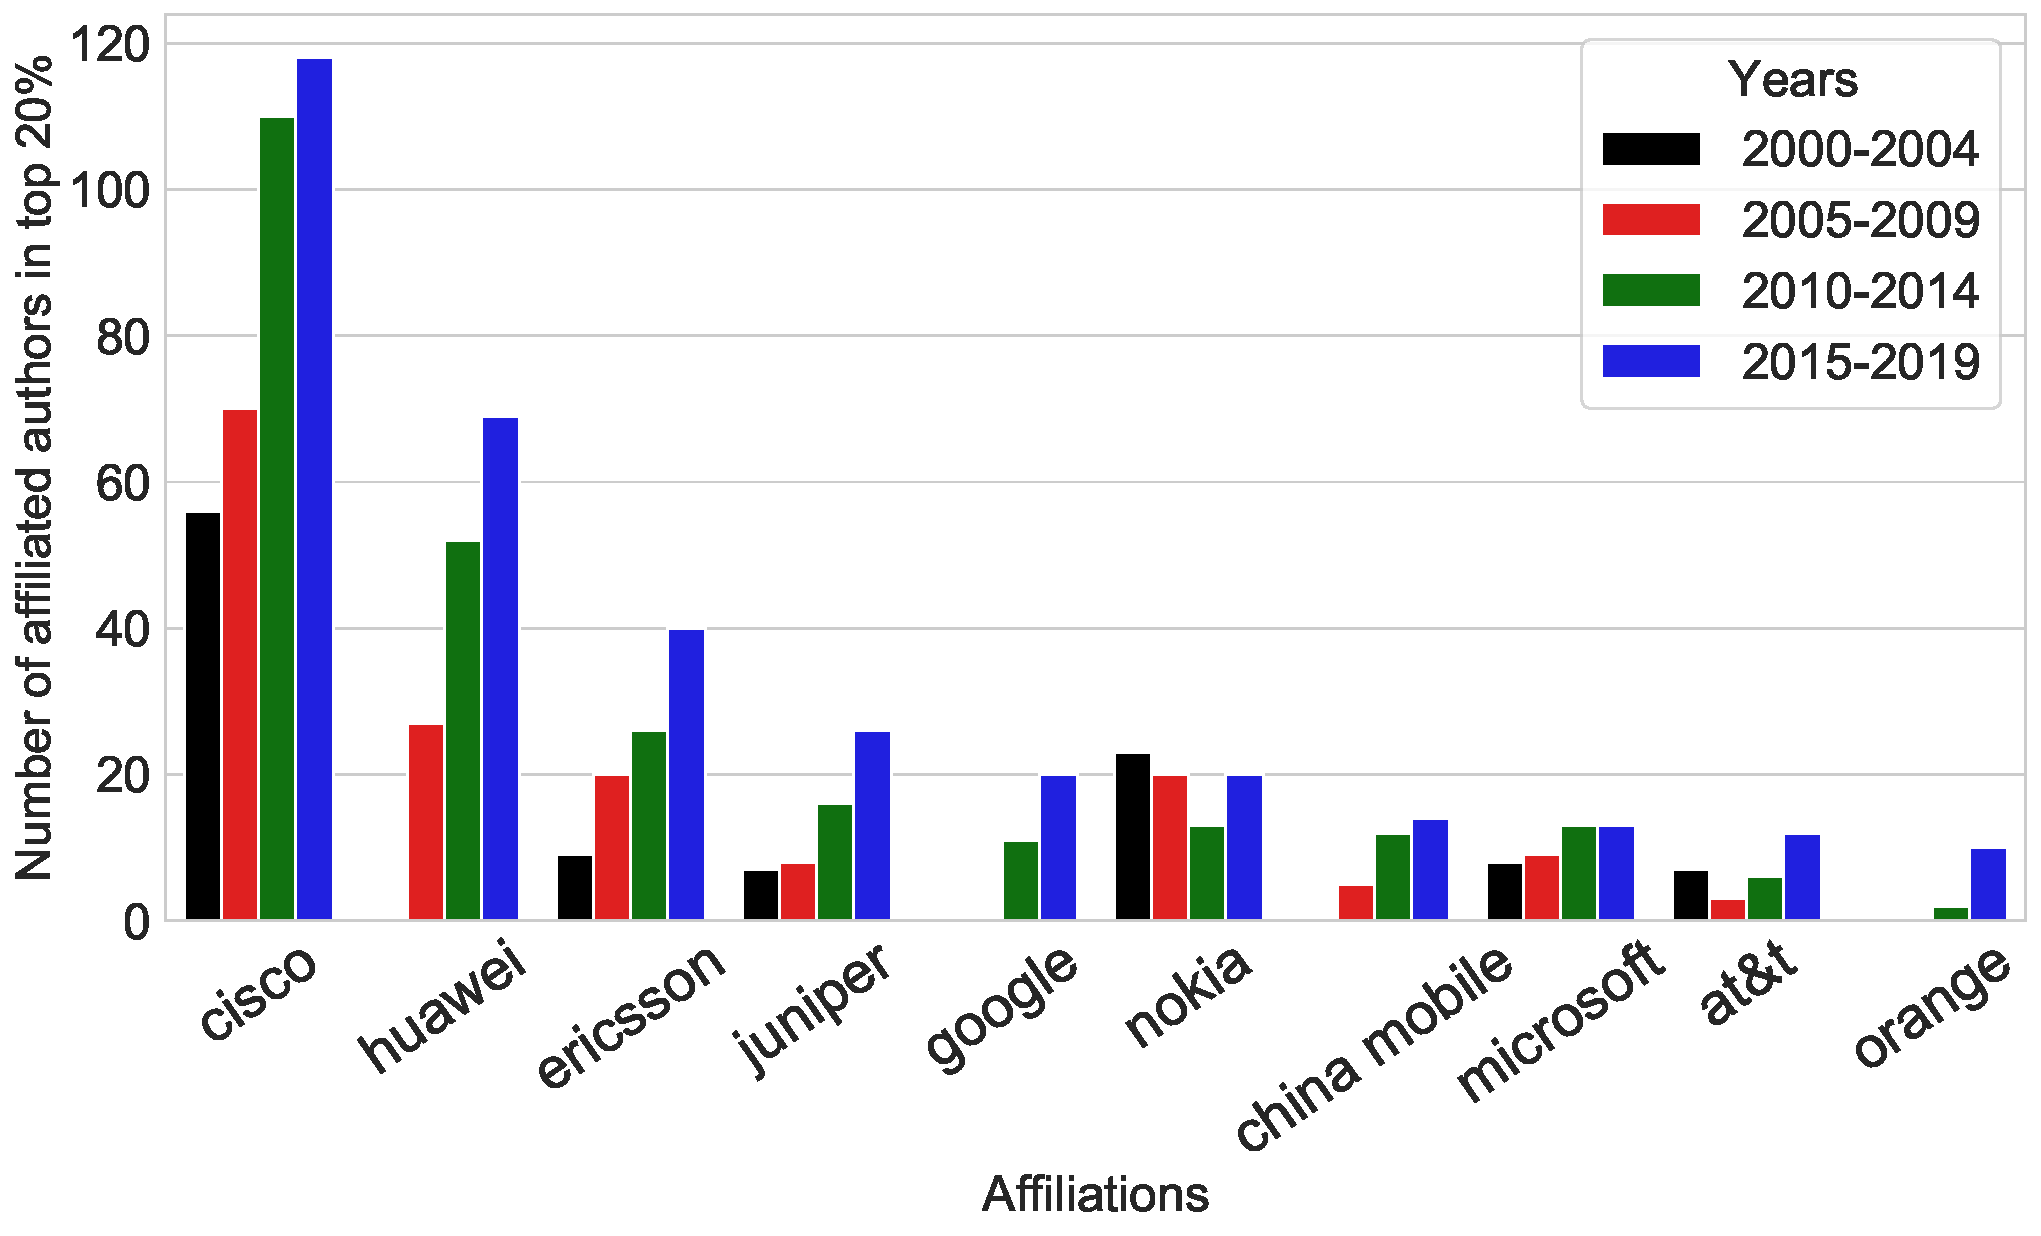
\includegraphics[width=\figureWidthOneColumn]{figures-prev/icwsm-2022/coauthor_affiliation_network/2019_affiliations_in_otheryears_coauthor_network.pdf}
  \caption{
    Authors in the most common affiliations of top 20\% authors
    (co-authorship graph) in 2015-2019.
  }
  \label{fig:coauthor_affiliation_network2019_otheryears}
\end{figure}

While authors from the same organisation often co-author drafts together,
collaborations between authors from different organisations are also
common.  Figure~\ref{fig:heatmap_2019_coauthordraft_most_frequent_org}
shows the most common collaborations between authors from the top 15 most
frequently affiliated organisations.  Collaborations between authors at
competing organisations, such as between authors from Cisco, Huawei,
Ericsson, and Juniper, occur frequently. We also computed that over the
years, joint collaboration (authors from multiple affiliations) has
increased: 772 co-authored drafts in the period 2000-2004 vs. 3083
co-authored drafts in the period 2015-2019.

\begin{figure}
  \centering
  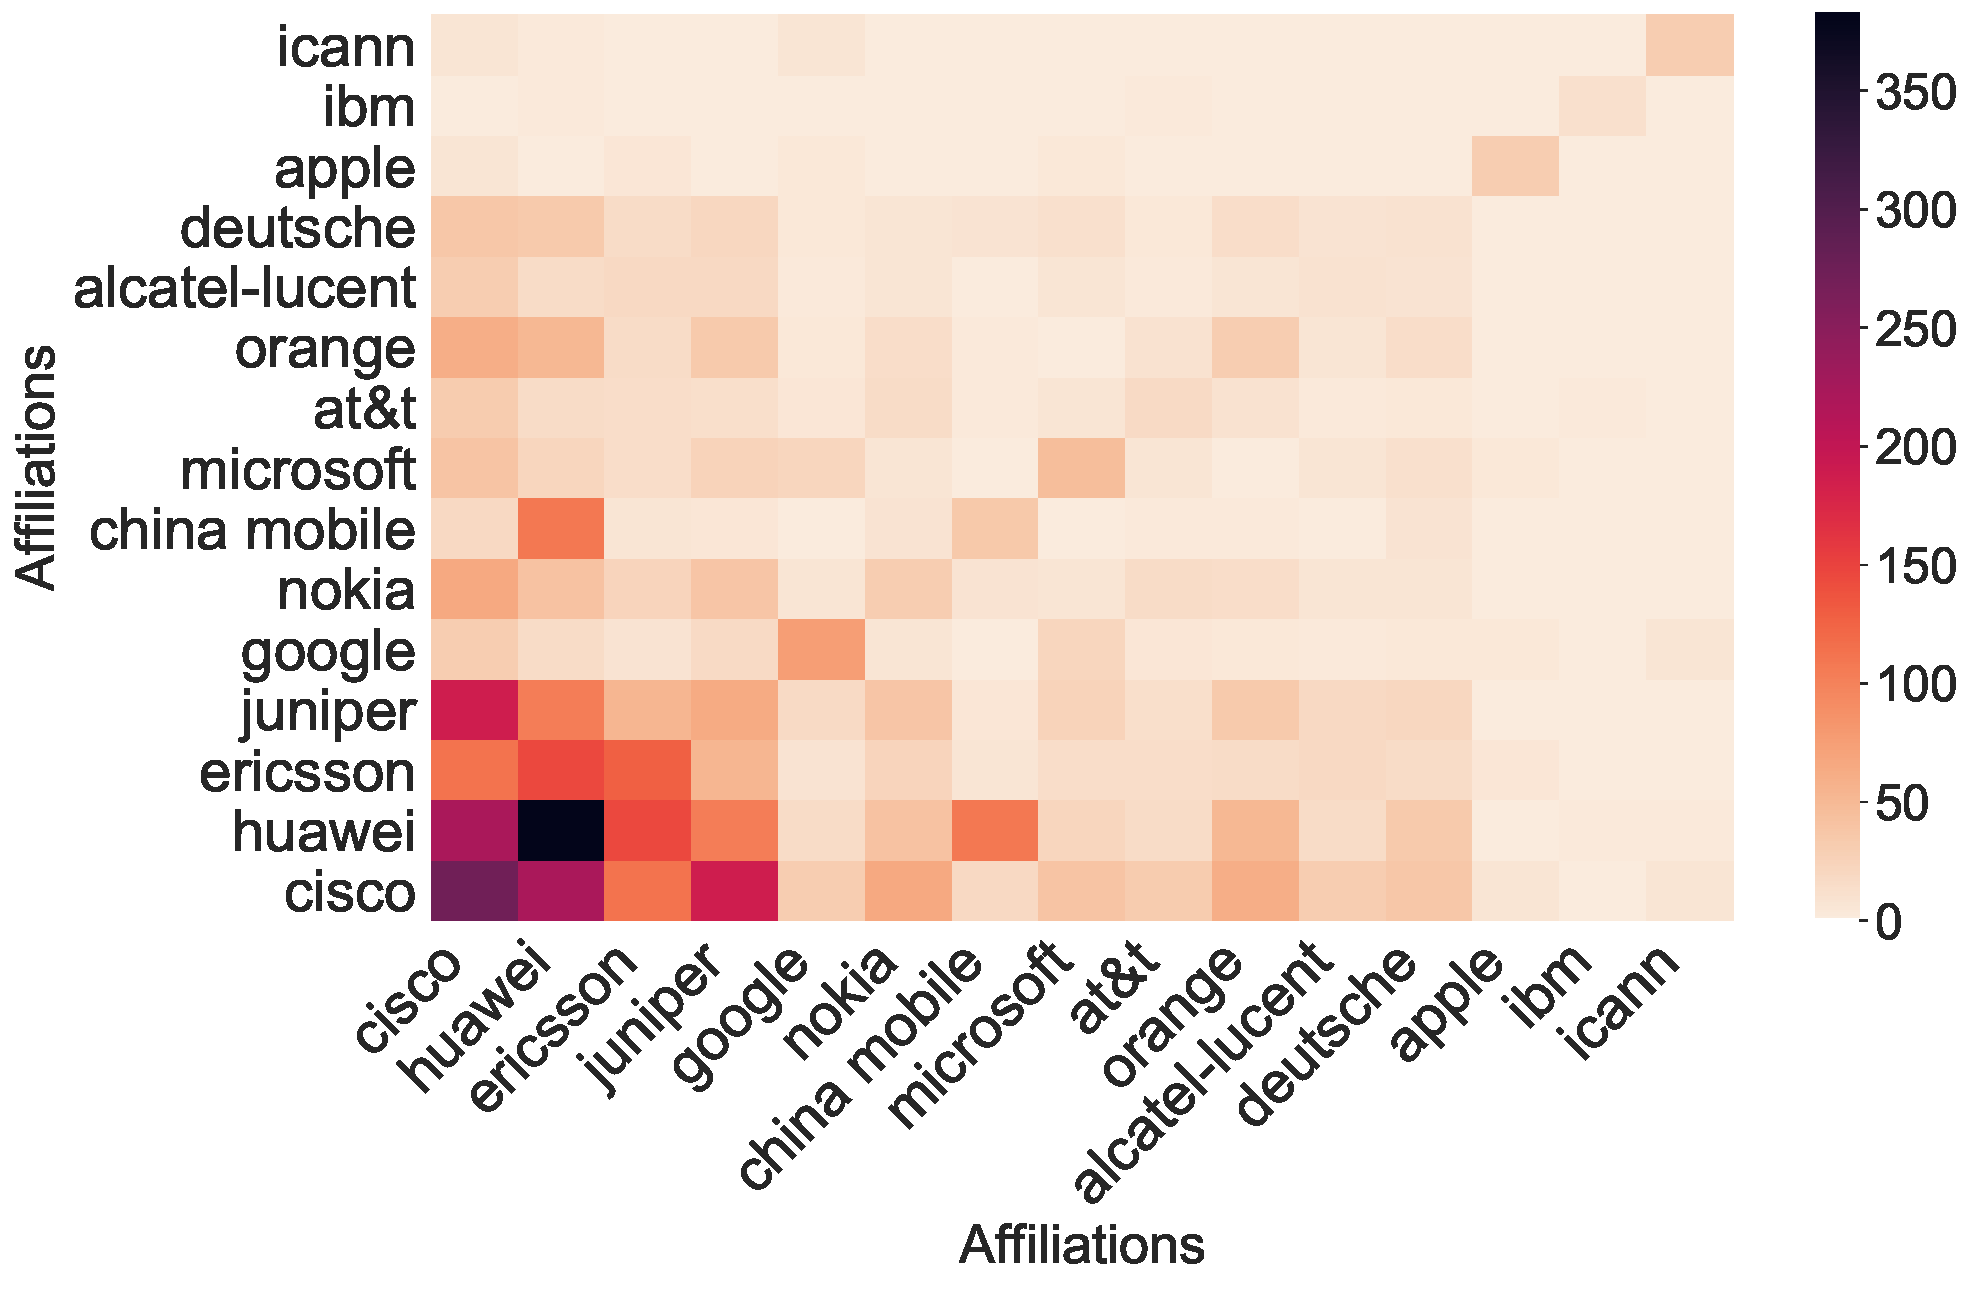
\includegraphics[width=\figureWidthOneColumn]{figures-prev/icwsm-2022/coauthor_affiliation_network/heatmap_2019_top10_affiliation_collaboration.pdf}
  \caption{
    Number of drafts co-authored by top 15 most frequently affiliated
    organisations. We only include the top 20\% authors (co-authorship
    graph) of 2015-2019.
  }
  \label{fig:heatmap_2019_coauthordraft_most_frequent_org}
\end{figure}

Further inspection of the collaboration trends reveals that the volume of
collaborations between authors from Huawei and other organisations appears
to be unaffected by the addition of Huawei to the U.S. Entity List
\cite{bis:2019:entity} as the trends in Figure 
\ref{fig:heatmap_2019_coauthordraft_most_frequent_org} also hold for 2020-2021.

% - - - - - - - - - - - - - - - - - - - - - - - - - - - - - - - - - - - - - - - - - - - - - - - - -
\subsubsection{Summary}

% ICWSM 2022 paper section 4.3

The IETF is a reasonably centralised organisation, that dominated by a
relatively small group of influential participants, but this dominance
is gradually reducing over time.
However, removing around 20\%-25\% most influential participants still
fragments the email graph (\S\ref{subsec:measuring_influence}, Figure
\ref{fig:purge_nodes_largest_connected_component_number_components}).

The most influential participants are those with the highest degree of
engagement within the community. These also tend to be more involved in
draft authoring (\S\ref{subsec:influencer_behaviour}, Figure
\ref{fig:drafts_initiation_top_percentile}). However, we also observe that
over the years more people, even those less influential in the email
network, are getting involved in draft authoring activities (Figure
\ref{fig:drafts_initiation_top_percentile}). This shows that these
activities, while centralised to a certain degree, are still open to
contributions from the wider IETF community.

We observe that the influential participants show a much higher level of
engagement with the community (\S\ref{subsec:influencer_behaviour}). A
considerable proportion of total emails is sent by the top 10\% of
influential participants (Figure \ref{fig:emailcount_top_percentile}).
Compared to the rest of participants, they are active in more areas (Figure
\ref{fig:areas_participation_top_percentile}), are active within the IETF
for a longer period of time (Figure \ref{fig:age_top_percentile}), and
participate in a more diverse set of topics (Figure
\ref{fig:topic_diversity}). Finally, their influence extends from the
mailing lists to other activities such as draft authorship.

A significant overlap and correlation is observed between
influential authors from co-authorship network and email networks
(\S\ref{subsec:impact_influence}, Table \ref{tbl:correlation_sprmn}). This
shows that a large set of authors exhibit an ability to co-author drafts as
well as engage with participants on the email networks, thereby translating
their influence from email networks to co-authorship and vice versa. 

Finally, a considerable portion of influential participants ($\sim$30\%)
are affiliated with one of the more prominent organisations, e.g., Cisco
or Ericsson, (Figure \ref{fig:coauthor_affiliation_network2019_otheryears}).
Participants from different organisations do considerably collaborate
(Figure \ref{fig:heatmap_2019_coauthordraft_most_frequent_org}). Moreover,
the level of such collaboration is found to have increased with time. 


%--------------------------------------------------------------------------------------------------
\subsection{Hierarchy and Communication Patterns}
\label{sec:org-dyn:hierarchy}

% ICWSM 2024 paper
% - RQ1: Are higher levels of the hierarchy growing or becoming more
%   centralised? Are they associated with an increased domination of the
%   conversation? 
% - RQ2: What is the association between the organisation hierarchy and
%   general communication patterns?
% - RQ3: How do people with differing roles communicate with each other?
%   Does information flow “up” or “down” the hierarchy? 
% - RQ4: What is the impact that individuals have on their direct contacts’
%   activity over time? How does this vary across hierarchy level?

As a voluntary and consensus-driven \cite{RFC7282} standards development
organisation, one might expect the communication patterns in the IETF to
differ from those in businesses following a more traditional management
structure. Those in IETF leadership rules, whether working group chairs
or area directors, must lead by persuasion and example and have little in
the way of coercive power compared to a typical manager and this can be
expected to impact how they communicate.

In the following, we quantitatively determine the effect that organisational
hierarchy levels have on communication patterns throughout the IETF. 
% We model communication as a network where a node represents an individual
% and a directed edge represents a communication sent from one individual to
% another~\cite{panzarasa2009patterns,viswanath2009evolution,klimt2004enron}.
% By repeating the analysis across time, we can build a full temporal
% network~\cite{masuda2016guide} of communication interactions between people
% in the system.In this study we consider only the network structure and the
% status at that time of the individuals, not the content of messages. 
We study how the email communication is impacted by the hierarchical roles
of individuals. According to the IETF mission statement~\cite{RFC3935}, the
IETF is made up of volunteers who collaborate to develop consensus-based
technical standards. This collaboration should be evident in their
communication practises.

%..................................................................................................
% ICWSM 2024 paper section 2

We consider the following questions: 
\begin{enumerate}
  \item
    Are higher levels of the hierarchy growing or becoming more centralised?
    Are they associated with an increased domination of the conversation?
    (\S\ref{sec:org-dyn:hierarchy:rq1})

  \item
    What is the association between the organisation hierarchy and general
    communication patterns?  (\S\ref{sec:org-dyn:hierarchy:rq2})

  \item
    How do people with differing roles communicate with each other?
    Does information flow up or down the hierarchy?
    (\S\ref{sec:org-dyn:hierarchy:rq3})

  \item
    What is the impact that individuals have on their direct contacts'
    activity over time? How does this vary across hierarchy level?
    (\S\ref{sec:org-dyn:hierarchy:rq4})

\end{enumerate}

Question 1 relates to the \emph{steepness} of the hierarchy
\cite{anderson2010functions}, that may exhibit a high amount of centralised
decision making, compared to a more \emph{diffused} \cite{hussain2019voice}
hierarchy where a larger amount of people in higher levels stifle lower
level voice by creating ``bystanders'' who find it hard to speak up. In
general, the conclusions about steep hierarchies are confused, where some
papers conclude a positive and some a negative effect of steep hierarchies.
We explore what this means for the IETF in \S\ref{sec:org-dyn:hierarchy:rq1}.

Questions 2-4 relate to the \emph{power distance}
\cite{li2021does,duan2018authoritarian,guo2020inclusive} of
individuals, which is the number of hierarchy levels between people who are
communicating. The focus is on the impact this has on people's voice or
lack thereof when the distance is large versus small. The conclusions from
this research area usually suggest that even small power distances have a
large effect of reducing the voice of the lower of the two levels. We
tackle this for the IETF in three different ways in
\S\ref{sec:org-dyn:hierarchy:rq2} -- \S\ref{sec:org-dyn:hierarchy:rq4}.

The voluntary nature of the IETF offers a new perspective on these
questions.  We demonstrate that despite the hierarchy becoming more
diffused, participants in the higher levels in the IETF hierarchy perform a
facilitator role, promoting discussion with those they interact with and
receiving a benefit themselves as a result. We also show that higher level
participants tend to be a focus of discussion with remarks directed upward
toward them whereas Regular Participants engage more in group-discussion
with less focus on an individual.  This suggests that the IETF does not
conform to the notion that power distance has a negative effect on
communication, nor that a more diffused hierarchy reduces the voice of
lower levels.

% - - - - - - - - - - - - - - - - - - - - - - - - - - - - - - - - - - - - - - - - - - - - - - - - -
% \subsubsection{Methodology}
% \label{sec:org-dyn:hierarchy:methodology}
% 
% % From our ICWSM 2024 paper, section 4:
% 
% \todo{Do we need a separate methodology section?}
% 
% - - - - - - - - - - - - - - - - - - - - - - - - - - - - - - - - - - - - - - - - - - - - - - - - -
\subsubsection{Centralisation and Dominance}
\label{sec:org-dyn:hierarchy:rq1}

% RQ1: Are higher levels of the hierarchy growing or becoming more
% centralised? Are they associated with an increased domination of
% the conversation?

%..................................................................................................
% From our ICWSM 2024 paper, Section 2:

% The effect the steepness of an organisation's hierarchy has on the
% communication within is not well understood. This RQ is important because
% once we know whether the IETF hierarchy is becoming steeper, we can look at
% the effects this is having on the communication patterns of participants.

In this section, we look at the number of individuals that inhabit each
level of the IETF hierarchy and their communication patterns, and quantify
the evolution of the mailing list activity within each level of the IETF.
We find that the middle level, Working Group Chairs, is gaining in overall
proportion of activity, whilst activity of participants at the lowest level
is decreasing. The top level of the hierarchy, area directors, remains
constant in proportion. The increase in working group chair activity
coincides with an increase in the number of chairs per working group.

%..................................................................................................
% From our ICWSM 2024 paper, Section 5.1:

\pb{Role of Working Group Chairs:}
Figure \ref{fig:activity_proportions}(a) shows the number of participants
at each level of the hierarchy in IETF: Regular participants are the
largest contingent, comprising 90--86\% of active participants; this
proportion is decreasing over time.  The next level is Working Group
Chairs, comprising  6--10\% of active participants; this proportion is
rising and becoming more diffused over time, with about 15 regular
participants for every working group chair in the organisation in 2013
versus 8 participants per chair in 2021.  The top level is Area Directors
who consist of less than 1\% of the total active population of the IETF;
this stays constant over time.  

The fraction of emails sent by participants at each level of the hierarchy
is shown in Figure~\ref{fig:activity_proportions}(b). Individuals at higher
levels contribute a disproportionate share to communication and this share
is increasing over time, consistent with \S\ref{sec:org-dyn:influence}. A
smaller proportion of email are sent by regular participants at the same
time as the number of working group chairs is increasing, further
suggesting that the IETF hierarchy is becoming more diffused, in terms of
mailing list communication, which may make cooperation between hierarchy
levels more difficult.

\begin{figure}[t]
  \centering
  \small{a)} \\
  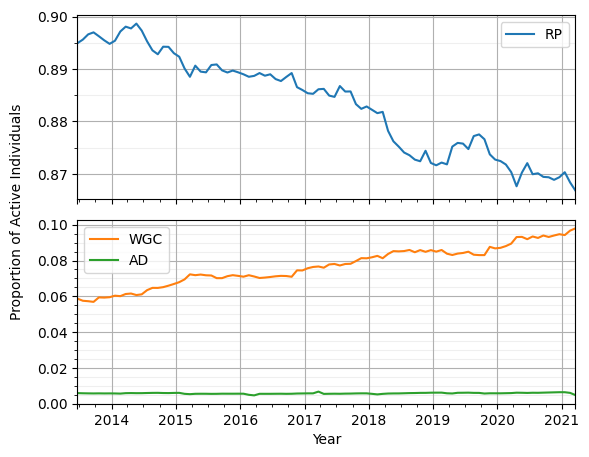
\includegraphics[width=\figureWidthOneColumn]{figures-prev/icwsm-2024/active_node_proportions_year_sliding_window.png} \\
  \small{b)} \\
  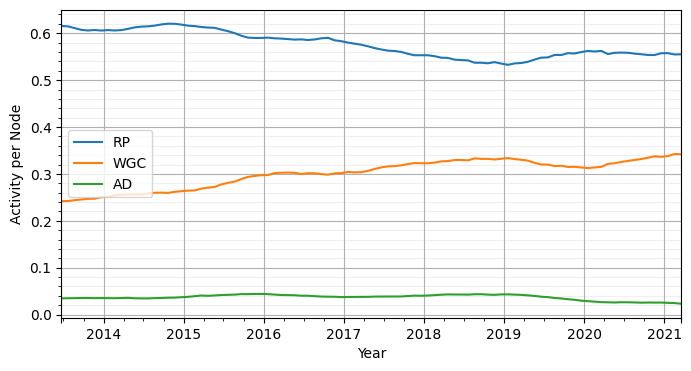
\includegraphics[width=\figureWidthOneColumn]{figures-prev/icwsm-2024/activity_proportions_year_sliding_window.png}
  \caption{
    Proportion of regular participants, working group chairs, and area
    directors by (a) number of active individuals and (b) mailing list
    activity.
  }
  \label{fig:activity_proportions}
\end{figure}

%..................................................................................................
\pb{Number of Working Group Chairs:}
Figure~\ref{fig:wgc_over_time}(a) shows the number of working group chairs
our time. There is a $35\%$ rise in the number of chairs while the amount
of individuals that fill the chair roles remains mostly constant.

Figure~\ref{fig:wgc_over_time}(b) contains two estimates of the number of
working groups over time, based on tracking group events (i.e., Datatracker
metadata) and mailing list activity since groups may be recorded as being
active but have no activity, and vice-versa.  The discrepancy between the
two estimates is the least (at most 10 working groups) from late 2014 to
early 2019. 

Figure~\ref{fig:wgc_over_time}(c) shows how many chairs exist per working
group, using both estimates of the number of working groups from
Figure~\ref{fig:wgc_over_time}(b). It is clear there is a slow a rise in
the number of chairs per working group over time. The ratio rises from
between 1.7-1.9 to 2.0-2.2 within the middle 50\%, late 2014 to early
2019.This perhaps represents a growing understanding in the IETF that it is
desirable to have two or more chairs per working group in case of
illness/unavailability or to avoid conflicts of interest. Therefore, this
plot again shows that the hierarchy is becoming more diffused, even if the
raw amount of individuals in the chair roles has remained constant. The
multiple roles per individual may result in even more difficulty of regular
participants to use their voice.

\begin{figure}[t]
  \centering
  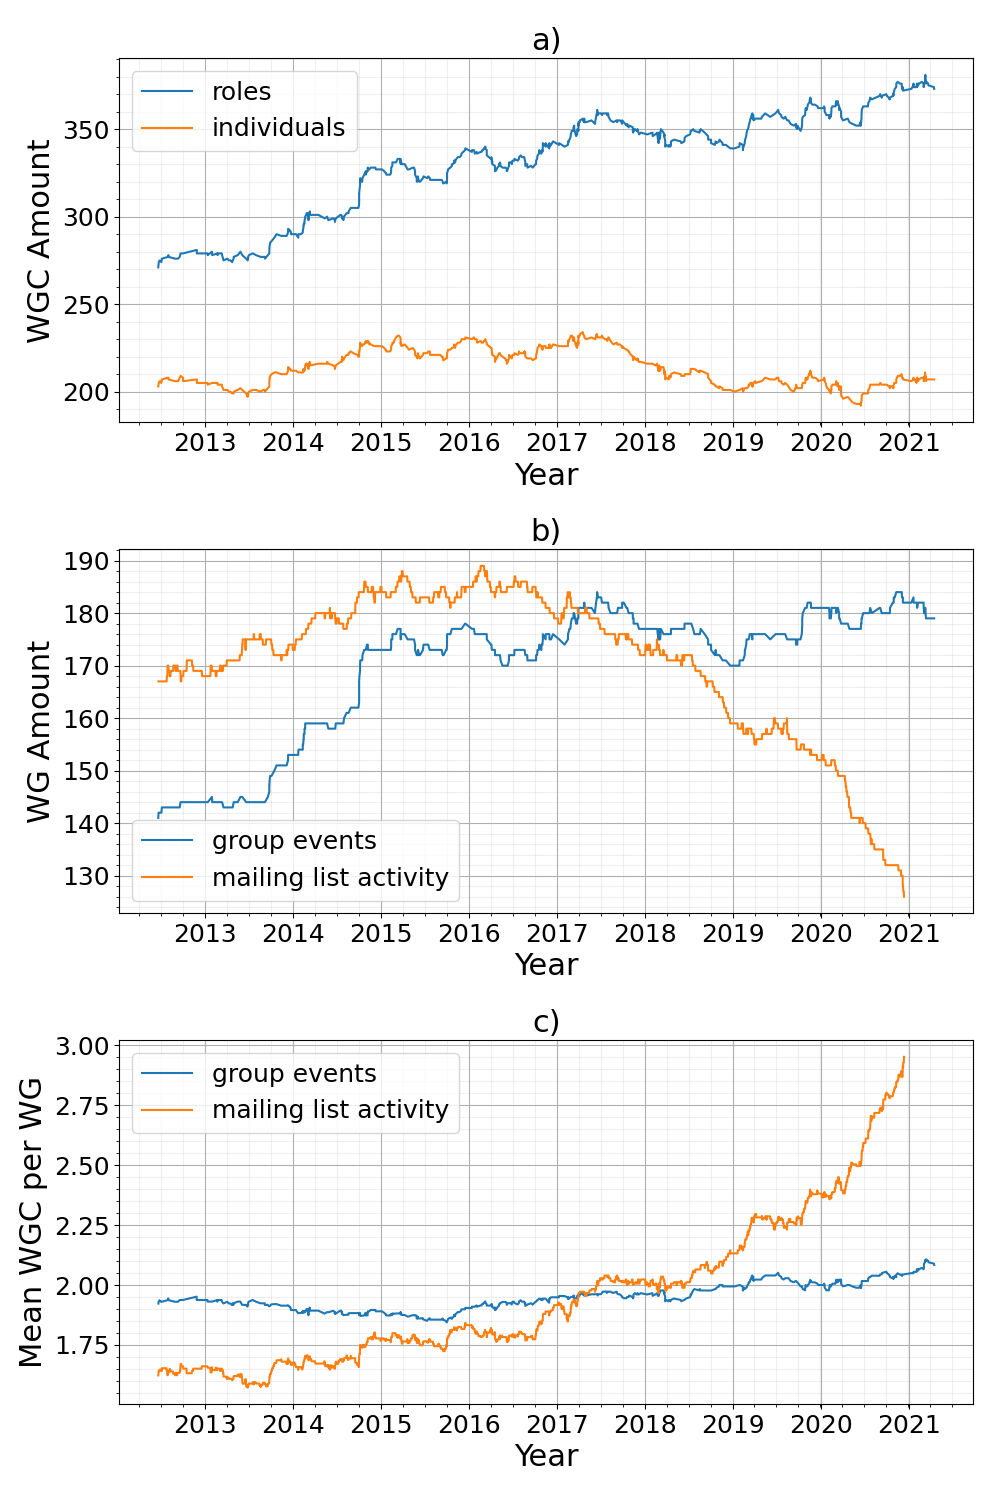
\includegraphics[width=\figureWidthOneColumn]{figures-prev/icwsm-2024/over_time.png}
  \caption{
    Changes in the number of working groups and working group chairs over
    time: (a) shows the number of chairs and the number of individuals who
    are chairs; (b) shows two different estimates of the number of working
    groups; and c) shows the mean number of chairs per working group.
    Notice the non-zero-based y-axis exaggerates the variation in these
    figures.
  }
  \label{fig:wgc_over_time}
\end{figure}

%..................................................................................................
\pb{Number of Area Directors:}
A version of Figure~\ref{fig:wgc_over_time} considering area directors
rather than working group chairs is available, but omitted to save space as
all three plots stay mostly constant throughout the period. There are about
15 area directors split amongst 15 roles in 7-8 areas with typically 2 area
directors per Area. The set of IETF Areas changes slowly, while working
groups are created and closed relatively frequently.

%..................................................................................................
\pb{Activity prior to appointment:}
Table~\ref{tab:WGC_email} shows the amount of email sent and received for
working group chairs and area directors on mailing lists in the year before
they first take that role, and the year after. Chairs and area directors
are both active in using the mailing lists, area directors much more so.
However, they don't become more active to any major degree after taking the
roles. This may suggest that the individuals who take on higher hierarchy
level roles are already contributing at a higher level.

\begin{table}[!tbp]
\centering
    \begin{tabular}{c||c|c}
        Status & Sent & Received \\
         \hline \hline 
        Before WGC & $67.26\pm99.80$ & $70.11\pm103.37$ \\
        \hline
        After WGC & $77.20\pm102.85$ & $85.90\pm107.38$ \\
        \hline
        Before AD & $218.84\pm226.92$ & $230.50\pm214.75$ \\
        \hline
        After AD & $209.21\pm186.46$ & $219.16\pm189.85$ \\
    \end{tabular}
        \caption{Mean number of emails received for one year before/after becoming a WGC (AD) for the first time. The error is one standard deviation.}
    \label{tab:WGC_email}
\end{table}

%..................................................................................................
\pb{Summary}
The answer to the question of whether the higher levels of the hierarchy
growing or becoming more centralised, and whether they're associated with
an increased domination of the conversation, is mixed.  The number of
individuals with working group chair roles has remained broadly constant
but the number of such roles has increased, indicating that individuals
willing to become chairs have taken on more such roles.  The number of the
higher level area director roles has, by design, remained broadly constant
over the time studied. The proportion of active individuals with working
group chairs roles has grown from 6\% to 10\% and the proportion of the
conversation taken by those roles has grown from 25\% to 35\% over the
period studied. Therefore the hierarchy has become more diffused, which may
mean regular participants experience more difficulty in expressing their
voice.


% - - - - - - - - - - - - - - - - - - - - - - - - - - - - - - - - - - - - - - - - - - - - - - - - -
\subsubsection{Organisational Hierarchy and Communication Patterns}
\label{sec:org-dyn:hierarchy:rq2}

% RQ2: What is the association between the organisation hierarchy and
% general communication patterns?

%..................................................................................................
% From our ICWSM 2024 paper, Section 2:

In this section, we explore communication patterns within the IETF, to
understand how participants in different roles (regular participants,
working group chairs, area directors) communicate and whether those
patterns of communication are indicative of healthy cooperation in the
running of the organisation \cite{li2021does,duan2018authoritarian}.

For instance, if those in leadership positions send lots of email while
receiving little, this suggests a lack of receptiveness of the leadership
to the suggestions from regular participants, and low confidence of those
regular participants to voice their opinions. In contrast, we hypothesise
that if the IETF operates as outlined in its mission statement, in a more
cooperative manner, then communication between those in different roles
will be more symmetric.

\pb{Temporal Motifs:}
We compare the ways that people in different roles communicate, looking
at the tendency for communications to be purely inbound, purely outbound,
or to follow more complex patterns. 
%
% From our ICWSM 2024 paper, Section 2:
%
We describe these in terms of \emph{temporal motifs}: patterns in the
sequence in which edges are added to the communication graph over time.
Specifically, we analyse every possible combination of three temporally
ordered links~\cite{paranjape2017motifs} between at most three nodes.
The time order in which the nodes occur is important.  The direction of
edge 1 is arbitrary, but every edge temporally after it has their direction
oriented with respect to it. 

Figure \ref{fig:motif_types} shows all possible types of interaction and
classifies them into five types: motifs with two nodes; ``Outward Star",
announcements or dissemination of information; ``Inward Star", questions or
condensing of information; ``Mixed Star", one-on-one discussion; and
``Triangle" is group discussion with no individual as the focus. Motifs
with only two nodes  are rare in this network and we do not present the
results.

\begin{figure}
  \centering
  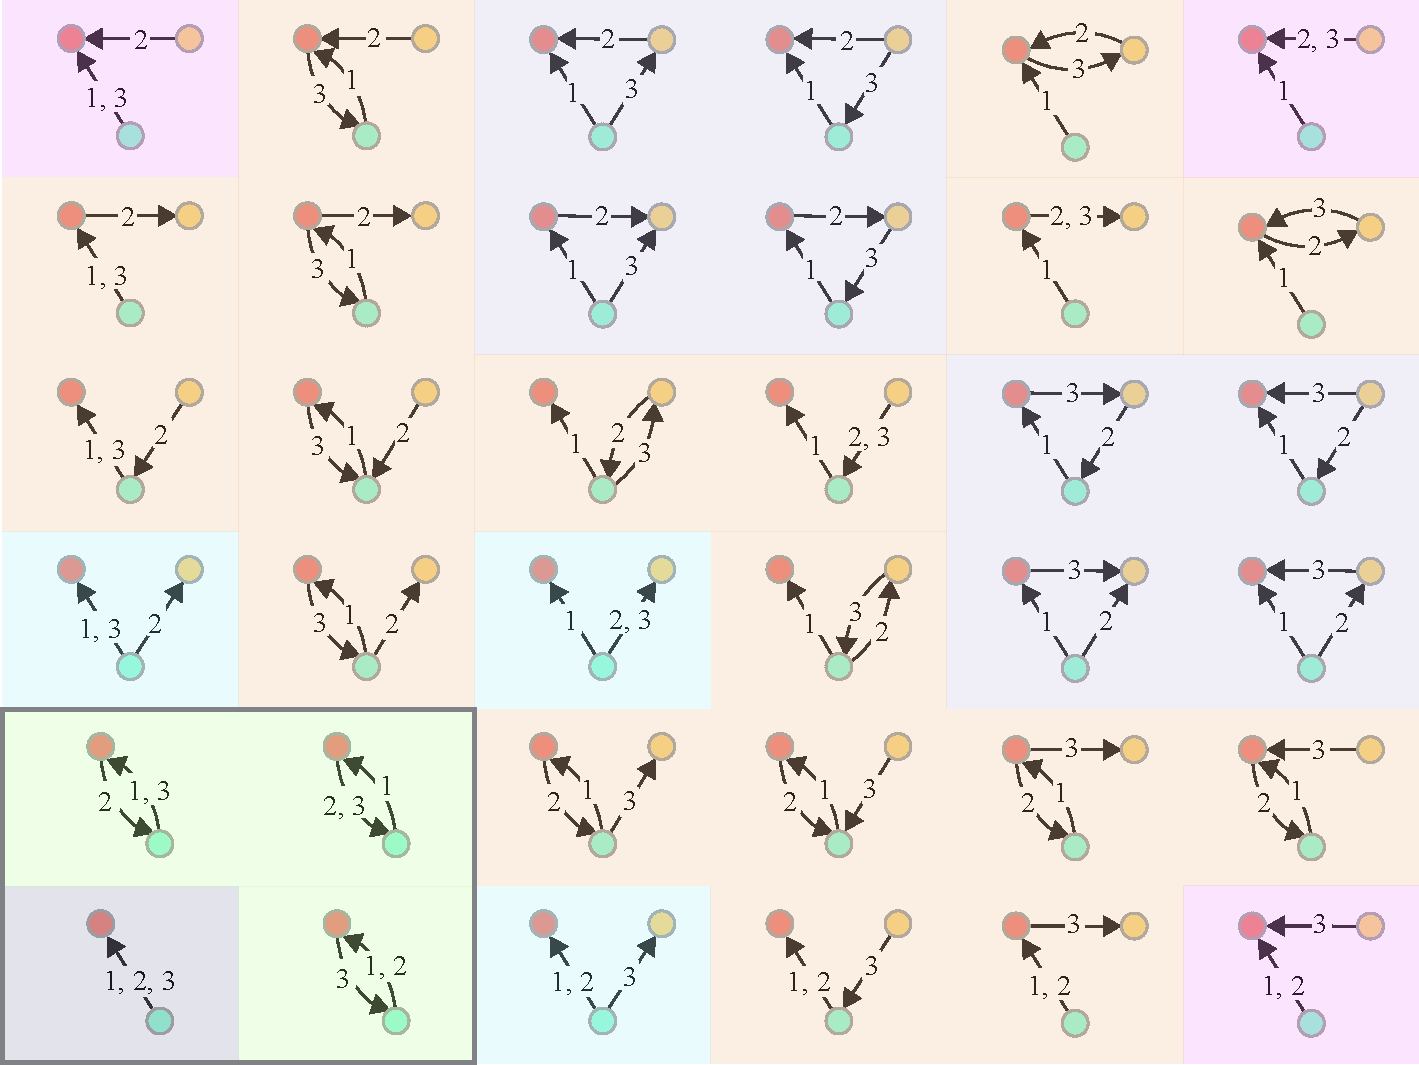
\includegraphics[width=\figureWidthOneColumn]{figures-prev/icwsm-2024/motifs.pdf}
  \caption{
    Classification of three edge motif types with the numbers representing
    the order of communication.  Light blue squares are  ``Outward Star''
    motifs; purple are ``Inward Star'' motifs; orange are ``Mixed Star''
    motifs and grey are ``Triangle'' motifs. The box in the bottom left hand
    corner represents motifs with only two nodes.
  }
  \label{fig:motif_types}
\end{figure}

Raphtory~\cite{steer2020raphtory} is used to count the prevalence of these
motifs. We start with the list of 36 different combinations of three
directed edges shown in figure~\ref{fig:motif_types}. The graph is then
split into time windows and then the motifs are counted combinatorially for
each window; each of a node's edges are followed from their origin to three
edge steps away. Finally, we combine the motif counts using the categories
shown in figure~\ref{fig:motif_types} by the colour of the squares.

% We find that those in leadership positions (working group chairs, area
% directors) consistently experience a higher proportion of incoming
% communication than regular participants, and all levels send outward
% communication at similar proportions over time. Also, the proportion of
% people who begin email threads are split by hierarchy level. Higher levels
% show a disproportionate tendency to originate email threads. 

%..................................................................................................
% From our ICWSM 2024 paper, Section 5.2:

\pb{Impact of Role on Communication Patterns:}
To quantify the effect of being in a leadership position has on network
wide communication, we calculate the proportion of three node temporal
motifs, lasting at most a month, in which each node participates over a
year period. These temporal motifs are counted, categorised into the three
hierarchy levels (regular participant, working group chair, area director)
and then proportions are taken of each temporal motif type. 

Figure~\ref{fig:motif_proportions} shows the proportions of each level for
three node ``Inward Star", ``Outward Star", ``Mixed Star", and
``Triangles". The Inward and Mixed Star motifs show about a $4\%$ and
$10\%$ increase in proportion for higher levels in the hierarchy versus
regular participants. However, about a $10\%$ increase for regular
participants is seen for Triangles versus working group chairs and area
directors, and Outward Star proportions remain similar for all levels of
the hierarchy.

The larger proportion of those in leadership roles in Inward and Mixed Star
temporal motifs, whilst Outward Star motifs remain similar for all levels,
suggests that those in leadership receive more direct communication. The
higher proportion of Triangle motifs for regular participants suggests
their discussion is more of a group activity, whereas working group chairs
and area directors have a larger proportion of one-on-one conversations.  
We therefore interpret the general communication patterns within the IETF
as a discussion amongst participants interspersed with questions sent to,
and announcements from, the working group chairs and area directors.  This
indicates some collaboration between layers and confidence of some regular
participants' to voice their opinions upwards.

\begin{figure*}[t]
  \centering
  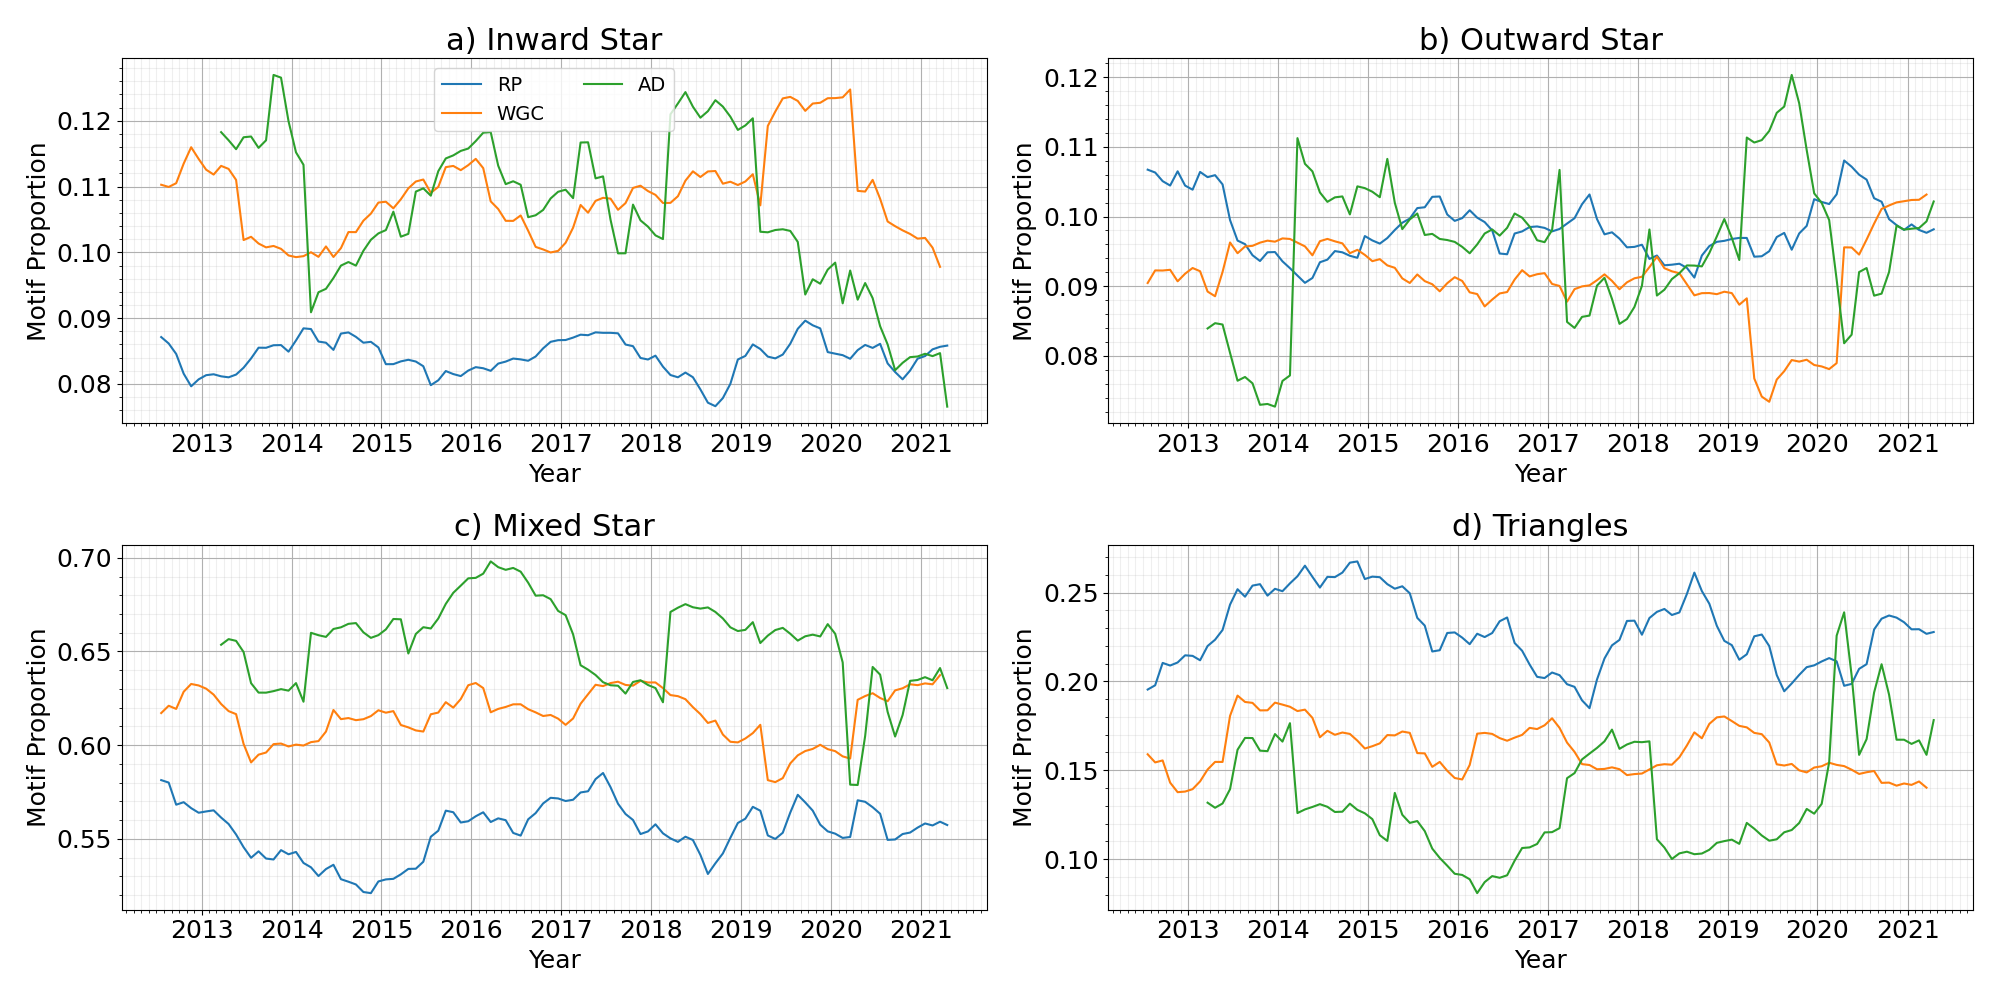
\includegraphics[width=\figureWidthTwoColumn]{figures-prev/icwsm-2024/motif_strata_comparison.png}
  \caption{
    Communication patterns analysed by three edge temporal motifs for RPs,
  }
  \label{fig:motif_proportions}
\end{figure*}


Figure~\ref{fig:origin_emails} seems to corroborate this. We calculate the
proportion of mailing list threads which nodes in each hierarchy level
originate, using a year window, pushed forward by a month each calculation.
We see that working group chairs and area directors send a disproportionate
number of originating emails to the mailing lists (working group chairs
send 30--50\% whereas they are 6--10\% of active individuals, and area
directors 5--10\% versus 0.5\%). 
Therefore, the larger proportion of inward motifs for those in leadership
roles is in part due to their disproportionately originating email threads.
Other IETF participants will then reply to the thread, boosting the
proportion of inward motifs working group chairs and area directors appear
in. This may suggest the higher levels are good ``condensers of
communication" as they receive more than they send.

\begin{figure}[t]
  \centering
  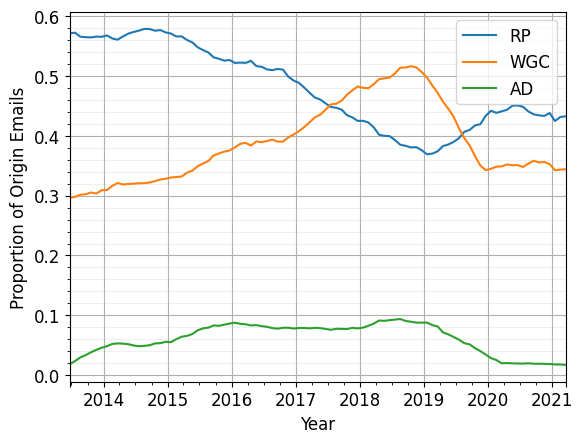
\includegraphics[width=\figureWidthOneColumn]{figures-prev/icwsm-2024/Origin_email_proportions.png}
  \caption{
    Proportion of ``origin" (non reply) emails sent by regular
    participants, working group chairs, and area directors, this should be
    interpreted in conjunction with Figure~\ref{fig:activity_proportions}
    showing the proportion of active individuals in each class.
  }
  \label{fig:origin_emails}
\end{figure}

\pb{Summary:}
Combining the interpretations of Figures \ref{fig:motif_proportions} and
\ref{fig:origin_emails}, the discussion seems to happen in the following
way: area directors or working group chairs are commonly the originators
of discussion threads. Where conversation includes a working group chair
or area director the conversation tends to be directed around them and
usually inward towards the working group chair or area director. The
regular participants are more likely to engage in discussions amongst
themselves (triangular communication patterns) when higher level
individuals are not present. 

% - - - - - - - - - - - - - - - - - - - - - - - - - - - - - - - - - - - - - - - - - - - - - - - - -
\subsubsection{Communication Up and Down the Hierarchy}
\label{sec:org-dyn:hierarchy:rq3}

% RQ3: How do people with differing roles communicate with each other?
% Does information flow ``up" or ``down" the hierarchy?

%..................................................................................................
% From our ICWSM 2024 paper, Section 2:

Our third hypothesis is that the cooperative nature of the IETF will be
evident in the effect that power distance~\cite{li2021does} has on
communication. The proportion of the communication between hierarchy levels
helps us to understand the confidence of lower levels to exercise their
voice: that is, the willingness of regular participants to challenge the
working group chairs and of the working group chairs to challenge area
directors.  This proportion, in a cooperative and voluntary organisation,
should be higher for those in lower positions in the hierarchy, showing a
confidence in their voice.

% We categorise edges based on the hierarchy levels they originate from and
% are sent to. Ratios are then calculated of ``upward'' versus ``downward''
% communication between regular participants, working group chairs, and area
% directors. We find that the lower the level, the more of a skew to upward
% communication.  Communication tends to flow ``up'' the hierarchy more than
% ``down''. 

%..................................................................................................
% From our ICWSM 2024 paper, Section 5.3:

We determine the direction communication tends to flow through the
hierarchy by looking at inbound and outbound communication flows. The
network's edges are categorised based on their source and target node's
hierarchy level. For each of the inter-level communication combinations the
proportion of communication in the last year going in the ``upward''
hierarchy direction is calculated. For instance, if there are six emails
from regular participants to working group chairs, and twelve from working
group chairs to regular participants, then the proportion upward is
$\frac{6}{6+12}=\frac{1}{3}$. 

In Figure~\ref{fig:inter_strata}, these proportions are plotted, and the
year long window is again pushed forward by one month to increase the
resolution of changes. A proportion of higher than $0.5$ shows more
communication flowing up the hierarchy than down. All three levels are
mostly upward in direction, with the lowest two levels (regular participant
$\rightarrow$ working group chair) having the largest skew in the
proportion. The other two lines (regular participant $\rightarrow$ area
director; working group chair $\rightarrow$ area director) show similar
periodicity, with the working group chairs $\rightarrow$AD line dropping as
far below $0.5$ as above showing a large shift in inter-level communication
patterns higher up the hierarchy.

\begin{figure}[t]
  \centering
  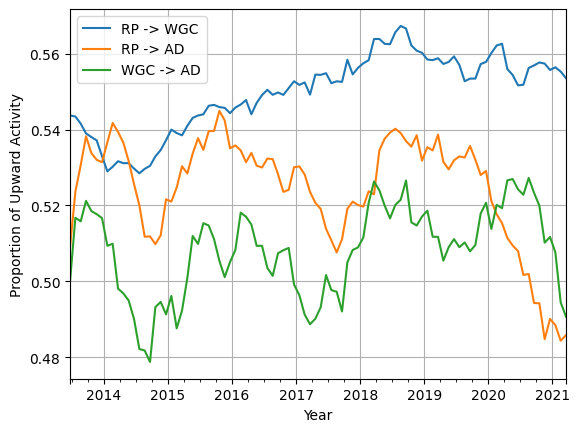
\includegraphics[width=\figureWidthOneColumn]{figures-prev/icwsm-2024/up_hierarchy_communication_ratios.png}
  \caption{
    Proportion of communications that are ``up'' the hierarchy for different
    groups. A proportion above 0.5 indicates that the majority of
    communications are ``upward''.
  }
  \label{fig:inter_strata}
\end{figure}

The direct measurement of message flow between the hierarchy levels seems
to bolster our interpretation that the cooperative design of the IETF is
working. This analysis shows that regular participants are communicating
much more preferentially upwards in the hierarchy, despite the decrease in
overall share of their activity. The increase within the working group
chair level does not have any noticeable effect on their level of
communication, if anything there is a negative relationship. This again
suggests both working group chairs and area directors perform a kind of
``condenser of communication'' or ``facilitator'' role. In other words,
this analysis suggests the IETF has a ``bottom-up'' communication style,
where the higher levels encourage the lower levels' voice.  This is the
desired pattern of communication for a volunteer organisation that is
looking to grow and encourage participants to engage and gradually take on
leadership roles.

\pb{Summary:}
The pattern observed was communication flowing up the hierarchy, broadly
matching that observed in \S\ref{sec:org-dyn:hierarchy:rq2}.  Working group
chairs and area directors were more likely to receive communication with
individuals than send communication to individuals whereas both were more
likely than regular participants to send out messages to the list in
general. 

% - - - - - - - - - - - - - - - - - - - - - - - - - - - - - - - - - - - - - - - - - - - - - - - - -
\subsubsection{Mobility Within the Hierarchy}
\label{sec:org-dyn:hierarchy:rq4}

% RQ4: What is the impact that individuals have on their direct contacts'
% activity over time? How does this vary across hierarchy level?

%..................................................................................................
% From our ICWSM 2024 paper, Section 2:

An important question for any organisation is whether higher level
participants encourage those at lower levels in the hierarchy to properly
engage \cite{li2021does,guo2020inclusive}. The IETF is cooperative and
voluntary by design, therefore we hypothesise a high level of encouragement
from higher levels to lower. We measure whether activity in one time period
is associated with activity in a subsequent time period both for
individuals and for neighbourhoods. If those who communicate with higher
levels receive a boost in their communication as a result, this is an
indication of such encouragement.

% In particular, we perform Mobility Taxonomy analysis to determine the
% effect individual IETF participants have on their future number of
% connections, and the average number of connections of their neighbours.  We
% find that working group chairs have an increased tendency, versus regular
% participants, to remain active (\textit{Mobility}), an increased tendency
% for their neighbours to be active subsequent to high working group chair
% activity (\textit{Philanthropy}) and for them to gain activity after their
% neighbours are active (\textit{Community}).  We interpret this as working
% group chairs filling a ``facilitator'' role on the mailing lists.


%..................................................................................................
% From our ICWSM 2024 paper, Section 4.3:

\pb{Mobility Taxonomy:}
We aim to measure the association of the activity of nodes, and their
neighbours, with their activity in a subsequent time period. To determine
this association we use the temporal graph analysis technique called the
Mobility Taxonomy~\cite{barnes2023measuring}, which involves correlating
the degree and average neighbourhood degree (ND) between two adjoining time
windows, both half of the chosen time window length for other analysis. The
temporal graph analysis tool Raphtory~\cite{steer2020raphtory} is used to
calculate the raw degree and ND numbers before performing these
correlations. 

There are six combinations to correlate node degree and ND in time window
one and two, the combinations are outlined in detail
in~\cite{barnes2023measuring}. The four measures used in this paper are
\textit{Mobility}, \textit{Neighbour Mobility}, \textit{Philanthropy} and
\textit{Community}.  Each represents the correlation of the degree of a
node (or set of nodes) at an earlier or later period of time.
\textit{Mobility} can be thought of as the tendency for a node that is
active in the first time window to be equally as active in the second.
\textit{Neighbour Mobility} is similar but for a node's neighbourhood.
\textit{Philanthropy} can be thought of as the tendency of a node's
neighbourhood to be active in window two if that node is active in window
one. Finally, \textit{Community} is the reverse of \textit{Philanthropy} as
the activity of a node in window two is compared to that node's neighbours
activity in window one.

Only the nodes which are active in the first window are considered for the
second window. Nodes inactive in the second time window are said to have a
degree of 0. The ND in the second time window is taken over the same set of
neighbours that existed in the first; that is we look at a node's
neighbours in the first window and measure their degree in the second for
consistency of comparison. 



%..................................................................................................
% From our ICWSM 2024 paper, Section 5.4:

\pb{Participant Mobility:}
To determine how individuals and their neighbours affect each other's
activity levels in subsequent time periods, we take correlations of degree
between different time windows using this Mobility Taxonomy. 
Figure~\ref{fig:mob_tax}, the time window chosen is one year which is split
into two snapshots graphs of six months, the time window then moves forward
one month and the process is repeated. The mid point of the year time
window is plotted. Working group chairs and regular participants are
plotted but the small number of area directors mean that the correlations
are too noisy to show meaningful effects. 

\begin{figure*}[t]
  \centering
  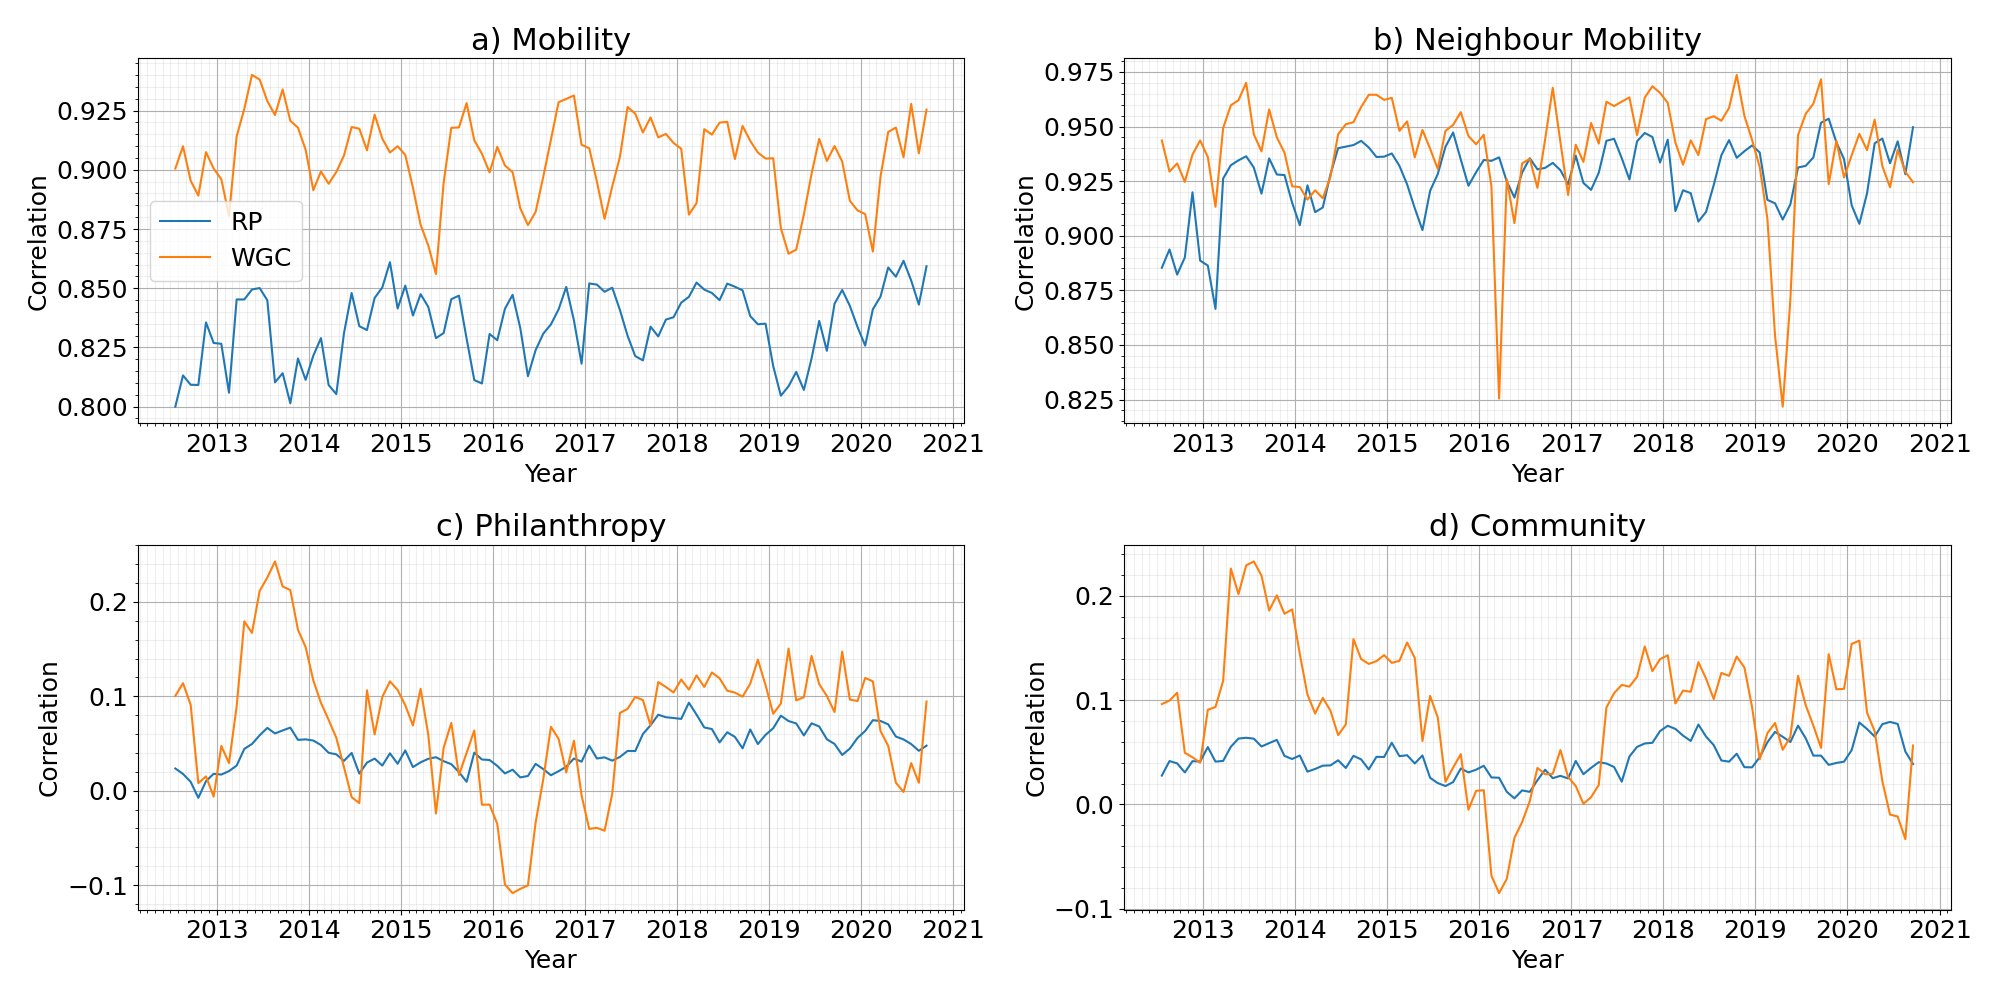
\includegraphics[width=\figureWidthTwoColumn]{figures-prev/icwsm-2024/hierarchy_status_comparison.png}
  \caption{
    Connection between roles and activity for regular participants and
    working group chairs viewed in terms of a) Mobility b) Neighbour
    Mobility c) Philanthropy and d) Community over time.
  }
  \label{fig:mob_tax}
\end{figure*}

The \textit{Mobility} of regular participants and working group chairs is
plotted in Figure~\ref{fig:mob_tax}(a). The high amount of correlation
between the degree of an individual in the first half of the time window
with the second half shows that all users have a tendency to become more
active in subsequent time periods if they are highly active in the previous
period, but this is more pronounced in working group chairs. This is found
to follow a period of about one year for both regular participants and
working group chairs, suggesting that a person is likely to be as active as
there were a year ago. The \textit{Neighbour Mobility} plot,
Figure~\ref{fig:mob_tax}(b), shows a similar tendency for neighbourhoods, but
with less of a split.

The \textit{Philanthropy} plot, Figure~\ref{fig:mob_tax}(c), shows a higher
correlation for working group chairs than regular participants between an
individual's degree in the first snapshot with and their ND in the second.
This means that individuals who directly interact with working group chairs
become more active on mailing lists subsequently. The \textit{Community}
plot, Figure~\ref{fig:mob_tax}(d), shows the correlation between the ND in
the first snapshot with the degree in the second.  The higher correlation
for working group chairs suggests they benefit from interactions with
highly active neighbours by themselves becoming more active in subsequent
time periods. These trends for \textit{Philanthropy} and \textit{Community}
show a reversal in early 2016 that coincides with a period where the mean
number of chairs per working group, and the number of working group chairs,
rapidly rising, see Figure~\ref{fig:wgc_over_time}. A merging of the
Applications area and Real-time Applications \& Infrastructure area in May
2015 may be a cause of this reversal of correlation, as the assignment of
working group chairs to areas was changed which may cause more non-reciprocal 
communication than normal.

%..................................................................................................
\pb{Summary:}
Increased \textit{Mobility} for working group chairs suggests that they
gain advantage from their role with their activity leading to similar
communication activity in the future. Moreover, they experience an
increased effect of \textit{Philanthropy} and \textit{Community}. The
former suggests that if a working group chair is engaged in a higher amount
of discussion, then in the future the individuals who they were
communicating with will also be highly active.  The latter suggests that
when working group chairs are surrounded by people who are active in
discussion, they are likely to be more active themselves in the future too.
All of this has less of an effect for regular participants who show a lower
correlation in terms of all three aspects. Our interpretation of this is
that active working group chairs are ``facilitating'' discussion in the WG
mailing lists; both having their activity boosted by their neighbours and,
in turn, boosting the activities of their neighbours. This aligns well with
the hypothesis that the cooperative and voluntary design of the IETF lends
itself well to higher levels encouraging those lower to engage in
discussion. 

Working group chairs have a positive effect on their immediate contacts.
Those individuals that directly discuss with working group chairs are more
likely to engage more in discussion in subsequent time periods.  Conversely
though the working group chairs who discuss topics with individuals who are
active in discussion are, themselves, more likely to engage more fully in
discussion. This points to something like a virtuous cycle of chairs
encouraging and being encouraged by their direct contacts. 

% - - - - - - - - - - - - - - - - - - - - - - - - - - - - - - - - - - - - - - - - - - - - - - - - -
\subsubsection{Summary}

% From our ICWSM 2024 paper, Section 6:

These findings presented in \S\ref{sec:org-dyn:hierarchy:rq2} --
\S\ref{sec:org-dyn:hierarchy:rq4} suggest that the negative association of
power distance is not as pronounced for the IETF as the literature finds
for traditional commercial organisations. In fact, the facilitation by
working group chairs of regular participants suggests the high levels
actively encourage lower level participation in discussion. 
Moreover, combining this with the finding that the organisational hierarchy
has a diffused structure (\S\ref{sec:org-dyn:hierarchy:rq1}), with the
potential problems this may cause for lower levels, suggests that
collaboration between hierarchy levels is high within the IETF.

As the IETF is voluntary and collaborative in its mission, this suggests
that the their process for tackling the problems caused by a diffused
hierarchy and power distance have worked well. One suggested improvement
for the IETF is to encourage working group chairs to get involved in more
group discussion in the mailing lists. This may help to boost their level
of \textit{Philanthropy}, \textit{Community} and Triangle motifs, which are
indicators of healthy discussion. However, we do not advocate for our
analysis techniques to be the only metrics maximised for.  Moreover, these
conclusions come from analysis of only communication structure not content.
A future look into content may elucidate differing relationships between
hierarchy levels.


%==================================================================================================
\section{Language and Influence}
\label{sec:language}

Moving on from discussing the people involved in the IETF (\S\ref{sec:trends-demographics})
and their interactions (\S\ref{sec:org-dyn}), we now consider communications
within the IETF from the perspective of language to explore whether there
are differences in linguistic patterns and language use in more influential
participants, and to consider how the use of language reflects the
consensus-driven nature of the standards development process.

% - - - - - - - - - - - - - - - - - - - - - - - - - - - - - - - - - - - - - - - - - - - - - - - - -
% The following is adapted from our ACL 2023 Tracing Linguistic Markers of
% Influence paper, section 2.

\pb{Linguistic Inquiry and Word Count} (LIWC) \cite{pennebaker2015development}
is a well-recognised psycholinguistic lexicon; it provides word counts for
85 different linguistic, psychological, personal concern, and informal
language marker categories. We generate a \emph{LIWC representation} of
the emails sent by a participant in the analysis that follows. This is
calculated by aggregating the word counts within each linguistic category
for each participant using the LIWC 2015 dictionary (academic license).
We filter out 104 ambiguous words that are present in LIWC but have
technology, security, and network context meaning in IETF, using manually
curated lists, for e.g., attack, argument, secure etc., 

We also normalise by the total number of emails sent by that participant. 
Such a normalisation is more appropriate here than normalising by total
number of words written, as many IETF emails include long technical
sections.  This generates a representation of a participant as their mean
usage of each LIWC category; while this is a relatively reduced,
low-dimensional representation of a person's language, it has the advantage
of being interpretable and psychologically well-motivated. 

A limitation is that we used the standard LIWC-based analysis approach,
which is purely lexical and does not take into account the context in which
a word appears. Consequently, many words that have very specific senses in
the context of the IETF get miscounted as occurrences of LIWC categories.
This could be addressed in future by a more advanced method of mapping to
LIWC categories that would account for context. 

%..................................................................................................
% The following is from our ACL 2023 Tracing Linguistic Markers of
% Influence paper RQ1: How do linguistic traits differ between more
% and less influential participants? 

\pb{Language and Influence:} How do linguistic traits differ between more
and less influential participants? That is, are there differences in the
way influential participants, based on centrality in the email social
graph, make use of language compared to those who are less influential?

We study mailing list data from the period 2015-2019, comprising 300,806
emails from 5,363 unique participants. We used a 5-year subset of the data
due to the computation cost, while still giving a reasonable period to
observe the participation consistency in the IETF community, and chose the
last period prior to the distortion of the pandemic.  For each participant,
we calculate the centrality-based influence score and LIWC representation,
We fit a linear regression model using LIWC representations to predict
influence percentile and observe the magnitude and directions of
significant coefficients.

The following LIWC categories are highly correlated ($p < 0.05$) with
centrality-based influence: \liwc{we, informal, risk, adjective, anger,
they}, and \liwc{bio}.  Categories such as \liwc{netspeak, sexual, health,
death, body} are correlated with lower influence. This suggests that
influential people tend to indicate a collaborative and community-oriented
approach with first-person plural (\liwc{we}) and third-person plural
category (\liwc{they}) usage. This is consistent with
\cite{kacewicz2014pronoun} and \cite{guinote2017power}, who show that
influential people use more first-person plural. They also use more
organisational language, which is shown by the negative correlation of
informal slang language categories (\liwc{netspeak, sexual, body}). We see
some unexpected hidden trends due to word ambiguity (e.g., words like
`\textit{trust}' and `\textit{live}'), which are discussed below.

%..................................................................................................
% The following is from our ACL 2023 Tracing Linguistic Markers of
% Influence paper RQ2: How do linguistic traits vary for participants
% at different levels of the organisation hierarchy? 

\pb{Language and Organisational Role:}
How do linguistic traits vary for participants at different levels of the
organisation hierarchy? 

Centrality-based influence considers participants based on their email
network, but role-based influence, based on the position of a person in the
organisational hierarchy (regular participant, working group chair, area
director) is equally crucial as they are involved in organisational
decision making.\footnote{In the top 10\% \textit{mail-based} influential
participants, less than 30\% are WG chairs with significant
\textit{role-based} influence.} 
For the same time period, 2025-2019, we split the data into two categories:
(a) emails sent by working group chairs, and (b) emails sent by regular
participants who have never been a working group chair (the number of area
directors is small, so we exclude them from this analysis).  We calculate
the LIWC representations for each person, train a logistic regression model
to predict category, and observe the LIWC category coefficients.


From \ref{table:all_results}, we see that working group chairs are more
social and collaborative, as is shown by \liwc{we} and \liwc{social}
categories. This is in line with our findings for influence-based
centrality above and resuslts on leadership engagement from the literature
\cite{strzalkowski2012modeling, liu2022pronoun, kacewicz2014pronoun,
guinote2017power}.
Chairs also use more tentative statements (\liwc{tentat}) in discussions,
primarily focused on technical feedback and revisions, or suggesting
alternatives. For example:
\textit{``With the risk of disturbing with statements, but avoiding too
many questions:This \underline{seems} against the goal of reducing
headers.''} 
and
\textit{``Question is do we need to carry around an outer IP-in-IP header
for that \underline{or} not?''}.

\begin{table*}[]
  \small
  \begin{center}
  \begin{tabular}{l|l|l}
  \toprule
    \multirow{2}{*}{Language and influence} 
      & High influence
      & \liwc{bio, we, informal, they, negemo, anger, risk, adjective}  \\ 
    \cmidrule{2-3}
      & Low influence
      & \liwc{sexual, death, ingest, netspeak, health, female, body, affiliation, conj} \\ 
  \hline
    \multirow{2}{*}{Language and role} 
      & WG Chair influence
      & \liwc{tentat, ipron, social, see, feel, we} \\
    \cmidrule{2-3}
      & non-WG Chair
      & \liwc{cogproc, relativ, affiliation, i, reward} \\
  \hline
    \multirow{2}{*}{Changes in Language}
      & Top 10 percentile
      & \liwc{adverb, prep, anger, auxverb, male, cogproc, achiev, risk, focuspresent} \\
    \cmidrule{2-3}
      & Below 50$^{th}$ percentile
      & \liwc{function, ppron, shehe, ipron, number, certain, sexual, informal} \\
  \hline
  \end{tabular}
  \end{center}
  \caption{LIWC categories where $p<0.05$.}
  \label{table:all_results}
\end{table*}


%..................................................................................................
% The following is from our ACL 2023 Tracing Linguistic Markers of
% Influence paper RQ3: How does linguistic behaviour of participants
% change as they gain influence?

\pb{Changes in Language with Changes in Role:}
Finally, we look at how linguistic behaviour of participants changes as
they gain influence in the IETF.
We consider at participants who went from low to high influence over time:
individuals who had a \emph{centrality-based} influence below the 50th
percentile when they joined the IETF, and reached the top 10th percentile
at some point.

For each participant, we generate two different representations based on
two periods---the year of joining, and year of reaching the top 10th
percentile for the first time---and assign these to two different classes.
We then train a logistic regression model to predict these classes, and
examine the coefficients of the LIWC categories

From Table \ref{table:all_results}, we observe that when participants
become influential, according to the centrality-based metric, they are
likely to be more descriptive and engaged in immediate state of issues
and situations as seen from the correlation of auxiliary verbs
(\liwc{auxverb}), adverb, risk, and present focus (\liwc{focuspresent}).
They are also more involved in cognitive processes (\liwc{cogproc}) as
compared to their previous self when they were new to IETF and had little
influence. 

%..................................................................................................
% The following is from our ACL 2023 Tracing Linguistic Markers of
% Influence paper, Section 4.2.
\pb{What Kinds of Language are Used?}
To better understand these LIWC categories and what kind of words play a
role in the behaviour of individual categories, we calculate the frequency
of words in each LIWC category as they appear in the emails. 
Next, we consider the top 30 most frequent words in each LIWC category and
perform regression analysis on centrality-based influence for participants,
but using only these 30 words as features to generate the participant
representation. We conducted this experiment separately for each LIWC
category that was significant in the first experiment.

From the word based analysis we make multiple observations. Firstly, words
like \word{we} imply a collective approach and is strongly correlated with
the higher influence. 
Similarly, the use of word \word{well} is standard, such as politely
resuming the conversation (e.g., `\textit{well, I agree}') or providing an
approval over something (e.g., `\textit{this works as well}'). These words
are well associated with the influential participants.  Otherwise,
influential participants are generally not observed to be informal and
other frequent words (other than \word{well}) within \liwc{informal}
category do not demonstrate a strong correlation with the growing
influence. Also, \word{well} is the most frequent word in the
\liwc{informal} category.

More influential people, according to both centrality- and role-based
metrics, are also observed to engage more with the community.
Conversations can often reflect situations where, as a part of review and
feedback process, more influential people highlight limitations in protocol
standards, stress on specifics, and compare with existing protocols or
previous versions.
Several words across different LIWC categories (\liwc{risk}, \liwc{negemo},
and \liwc{adj}) highlight such behaviour, e.g., \word{problems}, \word{before},
\word{particular}, \word{specific}, \word{different}, \word{most}, and \word{than}.

However, there are many words with dual sense, like \word{trust} which has
a very technology specific usage related to network security instead of
conversations involving trust issues between individuals or trust in any
given situation. Similarly, the word \word{live} is related with an
application or network being live, instead of its conventional meaning. We
also observed that some of the LIWC categories, such as \liwc{bio}, did not
have specific terms that could clearly establish its significance in favour
of influential participants (e.g., word \word{problems} and \word{trust}
reflecting the significance for the category \liwc{risk}), instead such
categories had several words with quite weak correlation with influential
participants. Such words collectively drifted the weight of the category
towards influential participants.

%..................................................................................................
% The following is from our Frontiers in Psychology paper:

\pb{Use of Sensitive Language:}
We briefly consider the use of sensitive language, relating to politics,
race, and religion, in IETF email communications.

Using email data for 2019, the last year prior to the pandemic, we
categorise the emails according to the role of their sender, based
on the relative social power of the sender within a working group:
\emph{working group chair} for emails sent by the current chair of the
working group to which the email was sent;
\emph{other chair} for emails sent by the chair of a different working
group; and
\emph{regular participant} for emails sent by people who were not, and had
not been at the time of sampling, a workgroup chair.
Due to their small numbers, we exclude area directors.

We use three LIWC categories to infer the presence of potentially sensitive
language in the emails: 
\liwc{Politics}---words commonly used in political discussions;
\liwc{Ethnicity}---words that identify national, regional, linguistic,
  ethnic, or racial identities; and
\liwc{Religion}--use of religious words.
Each email is coded according to the working group and role of the sender.
The emails are pre-processed to remove subject lines, headers, and any
embedded quotes from previous emails, yielding 101,857 texts by 2,300
individuals across 176 group mailing lists.  Each text is assigned a score
on each of the three language categories using the LIWC software and the
resulting scores are averaged for each individual sender for statistical
analysis.

Results are shown in Figure \ref{fig:sensitive}. The consistent pattern
is that people with organizational responsibilities (working group chair,
other chair) are less likely to use words potentially connected with
sensitive topics than regular participants without organizational
responsibilities, even though they are all part of the same discussions
on the same email lists.
Averaging across the two working group chair categories, the means indicate
that people in positions of social power are 3.2 times less likely to use
sensitive language overall than those who are not (by category:
\liwc{Politics} 2.0 times; \liwc{Religion} 2.3 times; \liwc{Ethnicity} 5.5
times).
It is worth noting, however, that in absolute terms potentially sensitive
language use is rare in this dataset, as might be expected for primarily
work-related communication. The modal LIWC score in both raw data and the
averages scores is zero

\begin{figure*}[t]
  \centering
  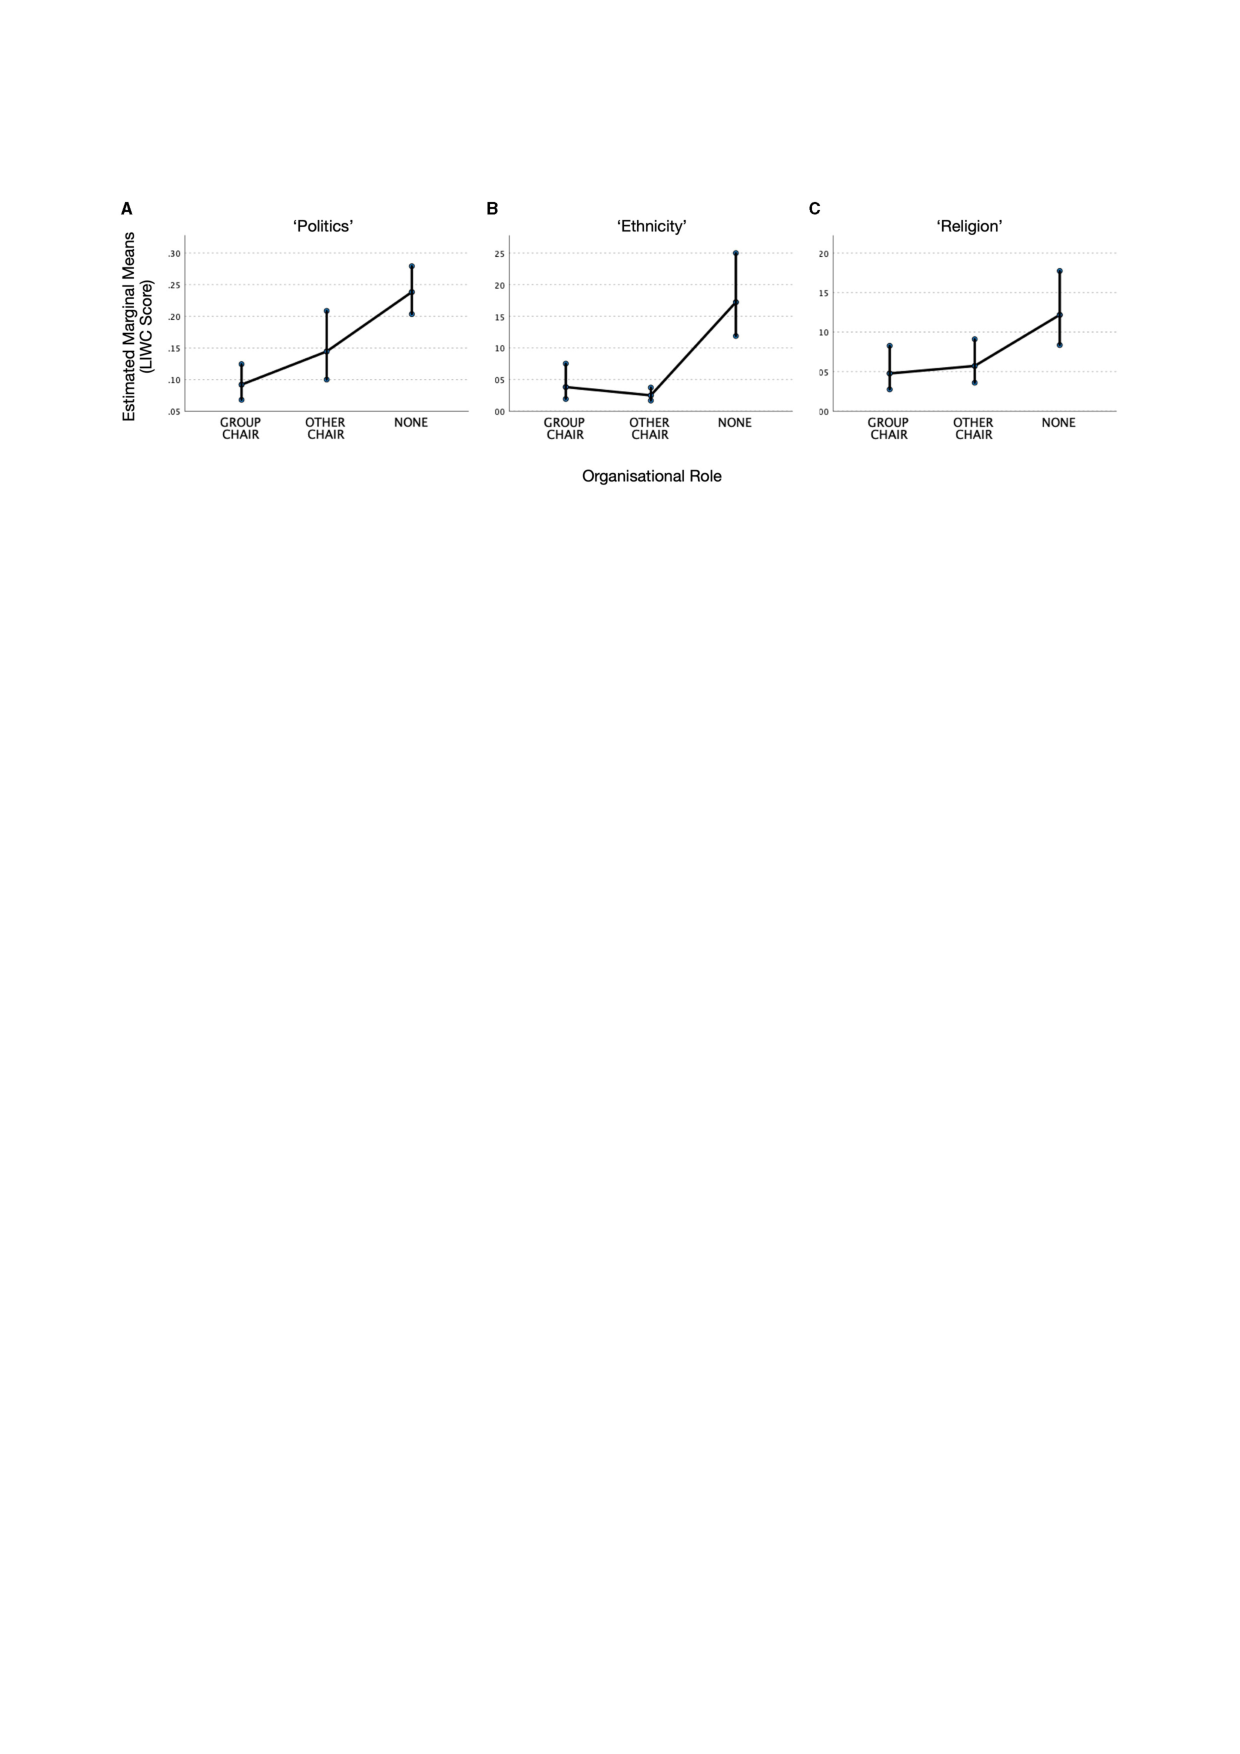
\includegraphics[width=\figureWidthTwoColumn]{figures-prev/frontiers/sensitive.pdf}
  \caption{
    Patterns of language use by organizational role. Estimated marginal
    means for the LIWC categories: (A) Politics, (B) Ethnicity, and (C)
    Religion. Error bars show 95% confidence intervals.
  }
  \label{fig:sensitive}
\end{figure*}

%..................................................................................................
% The following is from our ACL 2023 Tracing Linguistic Markers of
% Influence paper
\pb{Summary:}
Using two aspects of influence, based on centrality in the email social
graph and based on organisation role, we were able to unfold several
traits that differentiate influential participants from others. Many
of our findings seem corroborated by studies in organisational theory.
We observed that influential people exhibit more collaborative and
community-oriented traits, show stronger signs of engagement in
discussions, and are systematically less likely to use potentially
sensitive language.
We also observed that as people go on to become influential participants,
they evolve in their communication and are seen to be more engaging and
descriptive in their linguistic style. 


%==================================================================================================
\section{Success Factors}
\label{sec:success-factors}

Finally, we consider factors that lead to success, exploring what makes a
successful participant (\S\ref{sec:success-factors:authors}) and what makes
a document likely to be successfully published as an RFC (\S\ref{sec:success-factors:documents}).

Results show that influential authors (i.e., those with high centrality in
the email social graph) and authors affiliated with organisations that
participate strongly in IETF are more likely to have their documents
adopted and published as RFCs. However, documents that build on existing
work, have well-defined requirements, limited scope, and meet a need have
improved chances of success with authorships playing less of a role. Good,
well-connected, people are important, but so is focussed technical work.

%--------------------------------------------------------------------------------------------------
\subsection{What Makes a Successful Author?}
\label{sec:success-factors:authors}

% ICWSM 2022 paper Section 4

We have identified that influential authors write more drafts
(\S\ref{subsec:impact_influence}), but are these drafts more likely to
see success?  That is, does the presence of a well-connected, influential,
author make it more likely that an Internet-draft is adopted by a working
group for review and development\footnote{There are occasional document,
known as Area Director sponsored drafts, that are published as standards
track RFCs without going through the working group process, but these too
rare ($\sim$3\% of RFCs) to significantly affect our analysis.} and
eventually published as a standards track RFC.  Using information from the
IETF Datatracker we compile a dataset for the \emph{adoption} of a draft by
a working group, comprising 11632 drafts, and employ logistic regression to
analyse factors that affect working group adoption of draft.

%..................................................................................................
\pb{Methodology:}
We compute a set of features that may impact adoption or publication for
each draft, most of them motivated by the characteristics of influential
participants, including the following feature groups: 
 (1) \emph{text}, we derive a term frequency--inverse document
     frequency (TF-IDF) \cite{salton1983introduction} weighted bag of words vector
     representation of all email text of messages that either explicitly
     mention a draft or are part of a thread where the subject line
     explicitly mentions a draft; 
 (2) \emph{communication patterns}, i.e., volumes of incoming/outgoing communication
     between draft authors and IETF participants of varying experience levels;
 (3) Betweenness \emph{centrality} for authors;
 (4) \emph{number of emails} sent by authors;
 (5) \emph{number of drafts} submitted by authors;
 (6) \emph{length of participation} duration of authors;
 (7) \emph{number of authors};
 (8) \emph{number of IETF areas} in which the author is active;
 (9) \emph{proportion of top authors} in the top 10 and top 20 percent of
     influential participants;
(10) \emph{topic entropy ($\eta$)} scores for authors;
(11) \emph{author affiliations} for each of the 20 most influential
     organizations (20 boolean features);
(12) \emph{number of mailing lists} that each author participates in,
(13) \emph{number of years active}.

For numerical features that relate to each author individually instead of
the draft as a whole (e.g., \emph{number of emails sent}, \emph{centrality},
or \emph{number of years active}, the feature defined for each author
separately) in three variants: (i) for the least influential author, (ii)
for the most influential author, and (iii) as the average value across all
authors of the draft. We compute individual author features using
information from the 5-year period prior to draft submission.

Regarding the text based features, we found that the models tend to assign
high weights to words such as surnames of active contributors, names of
prolific working groups, and common technical terms. While this does make
the models perform slightly better, such terms should not be relevant for
solving the task as they do not model the relevant part of the conversation.
To explore how models would behave in a scenario wherein such words were
not available, we construct a domain-specific stop word list, consisting
of: (i) one all last names from the Datatracker, (ii) all working group
names from the Datatracker, and (iii) technological jargon terms obtained
from the web\footnote{\url{https://www.computerhope.com/jargon.htm}, we
used a union of the \emph{Internet terms}, \emph{network terms}, and
\emph{security terms} categories.}. We remove from this list any terms
appearing in top 5,000 English terms (e.g., sometimes people's names can have
identical surface forms as some of the terms relevant to organisational
activities). We will refer to this variant as \emph{text (S)}. 


To gain empirical insights into which features provide better prediction
results, models are run using a feature group alone variant and a variant
combining each feature group with the \emph{text} features. This approach
was motivated by the finding that \emph{text}, even though conceptually
quite different from the rest of the feature set and not our main focus,
does provide surprisingly strong results on its own. Thus, we wanted to
empirically investigate in more detail how well it complements the rest of
the graph-based features. Moreover, we compare all models to a baseline
which simply assigns all examples to the majority class.

We split the data into \emph{training} (70\%), \emph{development} (10\%),
and \emph{test} (20\%) subsets. As a scoring function, we use the F1 score
macro averaged across the positive and negative classes (but we also report
area under the curve (AUC), precision, and recall). We train the models on
the training set, optimise hyper-parameters on the development set, and
report final scores on the test set. The final scores are those obtained by
the model variant that fared best on the development set. We use logistic
regression implemented in \texttt{scikit-learn} \cite{scikit-learn}, given
that it is widely used and well interpretable. While we do not perform
explicit feature selection, we do have implicit feature selection through
L1 regularisation. We consider the regularisation strength a hyper-parameter
and consider values from $[2^{-7}, 2^{-6}, ..., 2^6]$ on the development
set. As our data set is quite imbalanced (in a roughly 4:1 ratio, 17\% is
\emph{adopted}), we use different class weights during optimization to
counteract this. We employ a non-parametric random shuffling test
\cite{yeh-2000-accurate} to check statistical significance of score
differences against the baseline. Table~\ref{tbl:res} summarises prediction
results, which will be discussed in the next section. 

\renewcommand{\tabcolsep}{0.5cm}
\begin{table*}
\centering
\begin{tabular}{lcccccccc}
\toprule
                        & \multicolumn{4}{c}{$\neg \mathit{TXT}$}
                        & \multicolumn{4}{c} {$\mathit{TXT}$} \\
\midrule
                       & AUC & F1 & P & R & AUC & F1 & P & R \\
\midrule
Baseline               &  .500 & .445 & .401 & .500  &  .500 & .445 & .401 & .500 \\
\midrule
Comm. patterns         &  .644 & .583 & .566 & .601 &  .723 & .626 & .609 & .644 \\
Centrality             &  .655 & .577 & .573 & .581 &  .717 & .639 & .625 & .653 \\
Email count            &  .632 & .566 & .555 & .577 &  .718 & .650 & .639 & .662 \\
N. years active        &  .608 & .569 & .555 & .584 &  .702 & .610 & .594 & .626 \\
Number of authors      &  .578 & .536 & .529 & .544 &  .697 & .631 & .621 & .641 \\
Proportion in top      &  .663 & .594 & .580 & .609 &  .728 & .634 & .614 & .655 \\
Draft count            &  .500 & .445 & .401 & .500 &  .696 & .630 & .624 & .636 \\
N. Areas               &  .634 & .572 & .557 & .588 &  .721 & .639 & .622 & .657 \\
N. Mailing lists       &  .634 & .570 & .557 & .584 &  .718 & .641 & .630 & .653 \\
Affiliations           &  .605 & .584 & .576 & .592 &  .708 & .626 & .609 & .643 \\
Topic entropy ($\eta$) &  .622 & .563 & .550 & .577 &  .715 & .642 & .628 & .657 \\
Text                   & - & - & -  & -  &  .681 & .624 & .622 & .627 \\
Text (S)               & - & - & -  & -  &  .667 & .598 & .593 & .614 \\
\midrule
All feats              &  .692 & .624 & .600 & .651 &  .744 & .645 & .625 & .666 \\
All feats (S)          &  .692 & .624 & .600 & .651 &  .726 &  .636 &  .627 &  .664 \\
\bottomrule
\end{tabular}
\caption{
  Results for predicting adoption. Each row presents the scores of a model
  using the corresponding feature group either alone ($\neg \mathit{TXT}$)
  or combined with the Text features ($\mathit{TXT}$). \emph{All feats}
  denotes all features except the text. Rows labeled with (S)  use the
  \emph{Text (S)} variant of the text features.
}
\label{tbl:res}
\end{table*}

Next, we wanted to confirm these results at the level of individual
features. To this end, we inspect the statistically significant
coefficients learned by the model corresponding to each individual feature.
For this experiment, we use a slightly different setup. We do not consider
the \emph{text} features\footnote{There are thousands of text features
(terms), making it prohibitively complex to include them. Moreover, they
are not central to our research questions about the IETF community.}. We
begin by first applying the Variance Inflation Factor (VIF) to exclude all
features with $\mathit{VIF} > 5$. This, to an extent, mitigates the
collinearity that we know exists as some features are by construction
highly correlated. We then standardise each remaining feature and then fit
a Logistic Regression model from the \texttt{statsmodels} package
\cite{seabold2010statsmodels} on the entire data set.
Table~\ref{tbl:resstat} presents the results of this experiment.

\renewcommand{\tabcolsep}{0.3cm}
\begin{table}
  \centering
  \begin{tabular}{lccc}
    \toprule
      Feature       & Weight  & P-value \\
    \midrule
      Centrality of most influential  & 0.1691 &   0.000 \\
      Centrality of least influential & -0.0698 &  0.048 \\
      Proportion of authors in top 10  & 0.1520 &  0.000 \\
    \midrule
      Has a Cisco author  & 0.1301 &  0.000 \\
      Has an AT\&T author  & 0.1003 &  0.000 \\
      Has a Juniper author  & 0.0738 &  0.000 \\
      Has a China Mobile author & -0.0697  & 0.000 \\
      Has an Alcatel-Lucent author  & 0.0474 &  0.022 \\
    \midrule
      Topic entropy max & 0.1728 & 0.000 \\
      Topic entropy min & -0.1135 &  0.002 \\
    \bottomrule
  \end{tabular}
  \caption{
    Weights of the model that are statistically significant at $p \leq 0.05$
    grouped by similarity of features -- author influence measures vs.\
    affiliation features vs.\ topic entropy ($\eta$).
  }
  \label{tbl:resstat}
\end{table}

%..................................................................................................
\pb{Predicting Adoption:}
To confirm empirical implications from Section \ref{subsec:impact_influence},
and provide a more in-depth look at the features, we perform statistical
analysis summarised in Table~\ref{tbl:resstat}. The most interesting
insight is that the coefficients corresponding to the \emph{Centrality of
the most influential author} and \emph{Proportion of authors in the top 10
percentile in influence}, are, indeed, positive and among the largest in
absolute value. This highlights that among the people who are influential
in the email networks, there is a substantial number of individuals who are
proficient in contributing to successful drafts.

Another interesting observation is that author affiliations (which are
also indirectly connected to influential participants, as demonstrated in 
\S\ref{subsec:impact_influence}, Figure \ref{fig:coauthor_affiliation_network2019_otheryears})
are an important feature group, particularly affiliations such as \textit{Cisco}
and \textit{AT\&T}. Moreover, topic entropy is also an important feature
group, which was also shown to be related to influential participants in
our analysis from \S\ref{subsec:impact_influence}, Figure \ref{fig:topic_diversity}. 

%..................................................................................................
% ICWSM 2022 paper section 4.3
\pb{Summary:}
The statistical analysis shows that influence of draft authors in the email
networks does impact the possibility of a draft getting adopted (Tables
\ref{tbl:res} \& \ref{tbl:resstat}). This might hint at the ability of
participants who hold a domain expertise to be able to engage better with
the community. Several WG chairs are already in the top percentile
influential category in both the email and co-authorship networks before
taking up these leadership roles, which further elevates after taking up
such leadership roles (Figure \ref{fig:wg_chair_before_after}).  Our
analysis also shows that being affiliated with a prominent organisation
positively impacts the chances of a draft in getting adopted by a working
group, thereby directly driving the innovation process (Table \ref{tbl:res}
\& \ref{tbl:resstat}).

%--------------------------------------------------------------------------------------------------
\subsection{What Makes a Successful Document?}
\label{sec:success-factors:documents}

% IMC 2021 paper Section 4

The trends that we observed in Section~\ref{sec:trends-documents}
highlight that, over time, the complexity of the standardisation process is
increasing: RFCs take longer to produce, and relate to a larger number of
other documents; authors come from a changing and diversifying set of
affiliations and countries; and the volume of email interaction for each
RFC is increasing, with differences in how senior and junior authors and
contributors interact.  We next seek to understand how these factors might
impact the successful deployment of an RFC in-the-wild, and to test if such
success can be predicted.

% IMC 2021 paper Section 4.1

We build on the work of Nikkhah et al.~\cite{nikkhah2017statistical}.
However, while the focus of that paper was on a set of features that were
derived from the standards documents themselves, we augment this with a set
of features derived from the author and email interaction datasets
described in the previous section.

To explore the factors that influence protocol deployment, we follow a
multi-step process:
\begin{enumerate}
  \item We reproduce the logistic regression model in~\cite{nikkhah2017statistical},
    to obtain similar results (as shown in Table~\ref{tbl:mlres}).
    That paper published an expert annotated dataset, labelling RFCs as
    ``successfully deployed'' or not. This pertains to whether the RFC was
    implemented in-the-wild and saw widespread (largely commercial) uptake.
    This dataset covers 251 RFCs published between 1983 and 2011, and
    includes 20 features. We create a baseline logistic regression model
    with $F_1 = 0.762$, $\mathit{AUC} = 0.650$. The results are similar to
    those reported in~\cite{nikkhah2017statistical} ($\mathit{AUC} = 0.670$).

  \item We curate a set of additional \emph{classification features} driven
    by our findings in Section~\ref{sec:trends-documents}. These are derived
    from the RFCs, their authors, and the mailing list interactions. Given
    that these features are only available for RFCs where Datatracker
    metadata is available, we model these features across a subset of the
    original labelled RFCs from~\cite{nikkhah2017statistical}, looking only
    at the 155 RFCs where all features can be calculated. We will show that
    modelling these RFCs with the expanded feature set substantially
    expands the predictive power of the (Step 1) baseline logistic
    regression model, with $F_1 = 0.820$, $\mathit{AUC} = 0.822$.

  \item We then train classification models to predict if an RFC will be
    deployed, using our expanded feature set.  We test the model with the
    manually labelled RFCs and show that we can successfully classify
    RFCs as deployed or not, with a decision tree-based model having
    $F_1 = 0.822$, $\mathit{AUC} = 0.838$. 
\end{enumerate}

\begin{table}
  \centering
  \begin{tabular}{lrrr}
    \toprule
      Model                              & $F_1$ & $\mathit{AUC}$ & $F1_{\mathrm{macro}}$ \\
    \midrule
      Most frequent class                & .757  &      .500      &     .379     \\
      Baseline                           & .758  &      .616      &     .597     \\
      Baseline + FS                      & .762  &      .650      &     .610     \\
    \midrule
      Most frequent class                & .724  &      .500      &     .379     \\
      Baseline                           & .670  &      .559      &     .547     \\
      Baseline + FS                      & .690  &      .620      &     .563     \\
      Logistic regression all feats      & .728  &      .724      &     .666     \\
      Logistic reg. all feats + FS & .820  &      .822      &     .789     \\
      Decision tree all feats + FS       & .822  &      .838      &     .788     \\
    \bottomrule
  \end{tabular}
\caption{
  Classifier scores on the entire dataset (251 RFCs, above) and those with
  our features available (155 RFCs), with or without feature selection (FS).
}
\label{tbl:mlres}
\end{table}


%..................................................................................................
% IMC 2021 paper Section 4.2
\pb{Classification Features:}
We begin with the set of features that were originally derived in
\cite{nikkhah2017statistical}:
IETF Area; Scope (Local, End-to-End (E2E), Bounded (BN), or Unbounded
(UB)); Type (New (N), New with Incumbent (NI), Backward compatible
extension (EB), or Extension (E)); Change to others (CO); Scalability
(SCAL); Security (SCRT); Performance (PERF); Adds value (AV); and Network
effect (NE). We refer the reader to~\cite{nikkhah2017statistical} for a
full explanation of each of these feature. 

We further define an additional set of document-based features, derived
from our characterisations in \S\ref{sec:trends-documents}: days from first
draft to RFC publication; number of drafts before RFC publication; number
of outbound citations to RFCs/Internet-Drafts; page count; number of
inbound citations from articles listed in Microsoft Academic, one and two
years after publication; number of inbound citations from other RFCs
published within one and two years after publication; RFC updates or
obsoletes a previous RFC; keywords per page; and topics (where we use
Latent Dirichlet Allocation (LDA) \cite{blei2003latent} to induce 50 topics
on the texts of all existing RFCs, and use the 50-dimensional probability
distribution over topics for a given RFC as the feature vector).

Next, we derive a set of author-based features, from the work described in
\S\ref{sec:trends-demographics}: number of authors on the RFC; if at least
one author of previously published  RFC; if at least one author in North
America, Europe, or Asia; if at least one author from Cisco, Huawei, or
Ericsson; authors with diverse affiliations; authors in more than one
continent;  at least one academic author; and at least one consultant
author.

Finally, we derive a set of features based on email interactions, from
\S\ref{sec:org-dyn:participants}: number of emails mentioning the
Internet-Drafts that precede publication of the RFC; mean number of emails
sent to all RFC authors, for each sender contribution-duration category
(young, mid-age,  senior); mean number of contributors sending emails to
any RFC author, for each contribution-duration category; number of emails
sent to most junior and senior RFC authors, for each sender
contribution-duration category; and number of contributors sending emails
to most junior and senior RFC authors, for each contribution-duration
category.

%..................................................................................................
% IMC 2021 paper Section 4.3
\pb{Modelling Methodology:}
With our expanded feature set, we next build a classifier to predict the
success (i.e., deployment) of RFCs.

Our expanded feature set, including all variants of each feature, is very
large, totalling 177 features. Given that our additional features can only
be calculated for a limited number of data points (155 RFCs),  it would be
infeasible to conduct statistical analysis, and to build a predictive
model, as there are too few data points. To address this, we take a number
of steps to reduce the feature space, while maintaining interpretability:

\begin{enumerate}
  \item Since the largest feature groups are the topics (50) and
    interaction features (54) we reduce both by applying the $\chi^2$ test
    to leave only the top 5 features in each group. 

  \item We remove collinearity by using the Variance Inflation Criterion
    (VIF), removing all features with a VIF value above 5. 

  \item We apply forward Feature Selection (FS) to identify features of
    high predictive value, following~\cite{nikkhah2017statistical}.
    Starting from an empty feature set, in each iteration of the forward
    procedure, we expand the feature set with the feature that provides the
    largest increase in the $AUC$ score. The procedure ends when there are
    no more unused features that yield score improvements over the current
    feature set. 
\end{enumerate}
The final set of features with and without FS is given in Tables
\ref{tbl:statsnofs} and \ref{tbl:statsfs} respectively.

Using the above feature set, we then train two classification models relying
on logistic regression and a decision tree.  For assessing predictive
performance of the models we use leave-one-out cross-validation, while for
the final statistical analysis we fit a logistic regression model on the
entire dataset and report the statistically significant coefficients (at
significance level $p \leq 0.1$).

\begin{table}
\begin{tabular}{lrr}
\toprule
Feature Name & Coef. & P>|Z| \\
\midrule
Change to others (CO) & 0.0001 & 1.000 \\
\textbf{Adds value (AV)} & \textbf{0.7828} & \textbf{0.009} \\
Security (SCRT) & 0.3830 & 0.253 \\
\textbf{Scalability (SCAL)} & \textbf{0.8755} & \textbf{0.100} \\
Performance (PERF) & 0.5108 & 0.323 \\
Microsoft Academic citations, 1 year & 0.2380 & 0.234 \\
Updates others (Yes) & 0.2877 & 0.514 \\
\textbf{Obsoletes others (Yes)} & \textbf{1.5315} & \textbf{0.001} \\
\textbf{Keywords per page} & \textbf{0.3409} & \textbf{0.083} \\
Inbound RFC citations, 1 year & 0.6112 & 0.011 \\
Junior-author $\rightarrow$ Senior (messages) & 0.1226 & 0.463 \\
Young $\rightarrow$ Senior-author (messages) & 0.2168 & 0.244 \\
\textbf{Senior $\rightarrow$ Senior-author (people)} & \textbf{-0.2902} & \textbf{0.096} \\
-00 draft mentions & -0.2198 & 0.187 \\
Final draft mentions & 0.1469 & 0.370 \\
All draft mentions (normalised) & -0.0504 & 0.755 \\
-00 draft mentions (normalised) & -0.1052 & 0.525 \\
Author count & -0.0941 & 0.561 \\
Days to publication & 0.1560 & 0.340 \\
Draft Count (DC) & 0.1845 & 0.262 \\
Outbound citation count & 0.2256 & 0.173 \\
\textbf{Page count} & \textbf{0.3468} & \textbf{0.054} \\
\textbf{Topic 13 (MPLS)} & \textbf{-0.5629} & \textbf{0.068} \\
Topic 19 & -1.2596 & 0.111 \\
\textbf{Topic 31} & \textbf{-2.0698} &\textbf{ 0.021} \\
Topic 44 & 0.3992 & 0.129 \\
\textbf{Topic 45} & \textbf{0.3289} & \textbf{0.097} \\
Area (INT) & -0.1671 & 0.683 \\
Area (OPS) & 0.5108 & 0.323 \\
Area (SEC) & 0.2231 & 0.638 \\
Area (TSV) & 0.5108 & 0.323 \\
Type, Backward Compatible (EB) & 0.3502 & 0.135 \\
\textbf{No incumbent} & \textbf{0.6061} & \textbf{0.039} \\
Has incumbent & -0.2007 & 0.655 \\
\textbf{Scope, End-to-end (E2E)} & \textbf{0.5878} & \textbf{0.035} \\
Scope, Local (L) & 1.3863 & 0.215 \\
\textbf{Scope, Unbounded (UB)} & \textbf{-1.0986} & \textbf{0.033} \\
Has author in N. America (Unknown) & -0.6061 & 0.232 \\
Has author in Europe (Unknown) & 0.1671 & 0.683 \\
\textbf{Has author in Asia (Yes)} & \textbf{-0.8755} & \textbf{0.100} \\
Has author from Cisco (Unknown) & -0.4055 & 0.442 \\
Has author from Cisco (Yes) & 0.4463 & 0.163 \\
Has author from Huawei (Yes) & -1.3863 & 0.215 \\
Has author from Ericsson (Unknown) & 0.0001 & 1.000 \\
Has author from Ericsson (Yes) & 0.5596 & 0.372 \\
Has continent diversity (Yes) & -0.1911 & 0.538 \\
Has an academic author (Yes) & -0.0870 & 0.835 \\
Has a consultant author (Yes) & -0.6931 & 0.423 \\
\bottomrule
\end{tabular}
\caption{Logistic regression w/o feature selection. Statistically significant rows ($p \leq 0.1$) are highlighted.}
\label{tbl:statsnofs}
\end{table}

\begin{table}
\centering
\begin{tabular}{lrr}
\toprule
Feature Name & Coef. & P>|Z| \\
\midrule
\textbf{Inbound RFC citations, one year} & \textbf{0.611} & \textbf{0.011} \\
\textbf{Obsoletes others (Yes)} & \textbf{0.531} & \textbf{0.001} \\
-00 draft mentions & -0.219 & 0.187 \\
\textbf{Scope, Unbounded (UB)} & \textbf{-1.0986} & \textbf{0.033} \\
\textbf{Has author in Asia (Yes)} & \textbf{-0.8755} & \textbf{0.100} \\
Has author in N. America (Unknown) & -0.6061 & 0.232 \\
\textbf{Keywords per page} & \textbf{0.3409} & \textbf{0.083} \\
\textbf{Topic 45} & \textbf{0.3289} & \textbf{0.097} \\
Has an academic author (Yes) & -0.087 & 0.835 \\
Type, Backward Compatible (EB) & 0.3502 & 0.135 \\
\textbf{Topic 13 (MPLS)} & \textbf{-0.5629} & \textbf{0.068} \\
\textbf{Topic 31} & \textbf{-2.0698} & \textbf{0.021} \\
Topic 44 & 0.3992 & 0.129 \\
Has continent diversity (Yes) & -0.1911 & 0.538 \\
Young $\rightarrow$ Senior-author (messages) & 0.2168 & 0.244 \\
Topic 19 & -1.2596 & 0.111 \\
Draft Count (DC) & 0.1845 & 0.262 \\
Scope, Local (L) & 1.3863 & 0.215 \\
Has author from Ericsson (Yes) & 0.5596 & 0.372 \\
\bottomrule
\end{tabular}
\caption{Statistical analysis using logistic regression w/ feature selection. Statistically significant rows ($p \leq 0.1$) are highlighted.}
\label{tbl:statsfs}
\end{table}


\begin{table}
  \centering
  \begin{tabular}{lrrr}
    \toprule
      Model & $F_1$ & $\mathit{AUC}$ & $F1_{macro}$ \\
    \midrule
      Most frequent class                & .757   & .500   & .379 \\
      Baseline                           & .758   & .616   & .597 \\
      Baseline + FS                      & .762   & .650   & .610 \\
    \midrule
      Most frequent class                & .724   & .500   & .379 \\
      Baseline                           & .670   & .559   & .547 \\
      Baseline + FS                      & .690   & .620   & .563 \\
      Logistic regression all feats      & .728   & .724   & .666 \\
      Logistic regression all feats + FS & .820   & .822   & .789 \\
      Decision tree all feats + FS       & .822   & .838   & .788 \\
    \bottomrule
  \end{tabular}
  \caption{
    Classifier scores on the entire dataset (251 RFCs, above) and those
    with our features available (155 RFCs), with or without feature
    selection (FS).
  }
  \label{tbl:mlres}
\end{table}


%..................................................................................................
% IMC 2021 paper Section 4.4
\pb{Evaluative Results:}
Using the trained models, we next evaluate their accuracy and explore which
features are most predictive of RFC deployment. 

As evaluative metrics, we use the $F_1$ score and the area under the ROC
curve ($AUC$), as in \cite{nikkhah2017statistical}. We find the standard
$F_1$ score gives overly optimistic performance estimates due the data
being skewed towards the positive class. Consequently, we also report an
$F1_{macro}$ score that takes into account both the positive and negative
class, reflecting performance more realistically. As a baseline comparison,
we present results of our re-implementation of \cite{nikkhah2017statistical}
using their feature set.

The prediction results of the models and feature sets are summarized in
Table \ref{tbl:mlres}. Our baseline model performs at a similar level to
that from \cite{nikkhah2017statistical}.  We further obtain considerable
performance improvements with our additional features. Furthermore, we find
that additional performance can be obtained by using feature selection.
The best performing model, with an F1 score of 0.822, is the decision tree
trained on the entire feature set.
Note, we also tested several non-linear models (neural networks, support
vector machines with non-linear kernels). These attained similar or worse
results as our decision tree model, and therefore we omit them due to space
constraints. 

We next investigate the most important features in predicting success.  We
posit that these can offer useful insight for working group chairs and RFC
editors.  The feature importance results are presented in
Tables~\ref{tbl:statsnofs} and \ref{tbl:statsfs}.  Some meaningful patterns
emerge here. We observe features such as adding value, being scalable,
obsoleting other RFCs, page count, increased keyword usage, no incumbent
RFC to compete against and limited scope all being positively correlated
with the likelihood of an RFC becoming deployed. In contrast, we find that
having a broad (unbounded) scope negatively impacts deployment.

We also observe some curious trends that speak to the limitations of our
dataset. The model finds that having an author in Asia is negatively
correlated with deployment, though with only borderline statistical
significance. Further analysis shows that only 10\% of labelled RFCs have
an author in Asia.  As shown in \S\ref{sec:trends-demographics}, we see
that demographics of the IETF are changing, with a recent notable increase
in author representation from Asia. This might suggest that new authors
need time to learn what makes a deployable protocol; equally our deployment
data may be biased towards the Internet in North America and Europe. This
finding requires much more exploration.

We further see that some of the topics extracted by LDA are also useful.
For example, Topic 13 is characterised by a cluster of terms associated
with MPLS, a widely deployed routing protocol. We find a negative
correlation with this topic, but this is likely because there is a
significant number of RFCs that propose modifications or additional
features for the protocol, some of which do not see deployment. Overall,
most of the results are in line with expectations, but more annotated data
is required for further insights.   

%..................................................................................................
% IMC 2021 paper Section 4.5
\pb{Discussion:}
% Building on existing work.
Features associated with building on existing RFCs positively correlate
with deployment. RFCs that obsolete earlier versions of the same protocol
are likely to be deployed, indicating that the IETF community is good at
identifying and maintaining protocols that are seeing use. This is also
highlighted by the significance of the inbound RFC citation and ``adds
value'' features. These show that RFCs that are later cited by other
documents, or that add value to other protocols in the stack, are more
likely to be deployed. Protocols that are extensible, and can be extended
and adapted for new uses, are more likely to see deployment. The discussion
in \cite{clark:2002:tussle} on careful choice of extension points
resonates; as do the implications for starting new work.

% Limited scope.
We find that having end-to-end scope (i.e., where only the endpoints of a
connection needs to implement the RFC) is positively correlated with
deployment, whereas having an unbounded scope (i.e., where the entire
Internet may need to be updated) is negatively correlated. This indicates
that well-scoped RFCs, that are cognisant of their deployment challenges,
are more likely to see deployment. A recent IAB workshop \cite{rfc8980}
noted that deployment often occurs in unforeseen ways: limiting the changes
needed to deploy a protocol facilities this.

% Normative requirements.
The number of keywords (e.g., SHOULD, MUST) used per page, which shows the
number of normative requirements an RFC imposes on implementations, also
correlates with deployment. This suggests that well-specified requirements
lead to robust, interoperable, implementations that see wide use.
Unsurprisingly, features such as citation rates are also predictive of
deployment.

% Diversity.
Notwithstanding the limitations of the dataset, we find that the majority
of author demographic features are not significant. While \S\ref{sec:trends-demographics}
identified recent shifts in the demographics of authors, these do not
appear to have a major influence in the deployment of the RFCs that they
write.

% Meeting a need.
Our results broadly support the conclusions of \cite{RFC5218}, where the
IAB noted that, in addition to being technically sound, a successful
protocol must meet a need, be incrementally deployable, and be open to
extension and maintenance.

%..................................................................................................
\pb{Summary:}
Our results show that RFCs that build on existing work, have well-defined
requirements, limited scope, and meet a need have improved chances of being
widely deployed. These document-based features have implications for how
the IETF should design and specify protocols.

We found that the majority of our author-based features, including
geographic and affiliation diversity, did not significantly impact the
deployment prospects of RFCs. Further work is needed to expand the dataset
to ensure that this result holds across a larger set of RFCs.

Finally, the focus of our modelling in this section has been on the impact of
document, author, and interaction-based features on protocol deployment.
However, this is only one part of the lifecycle of an RFC. It remains to
consider the impact of these, and other, features on the key stages of an
Internet-Draft's development towards becoming an RFC, such as working group
adoption.

%==================================================================================================
\section{Related Work}
\label{sec:related}

% This should come near the end, and focussing on discussing how your work
% relates to that of others. Any relevant related work should have been
% cited already, so this is not a list of related work, it's a discussion
% of how that work relates.
%
% Why not put related work after the introduction? 1) because describing
% alternative approaches gets between the reader and your idea; and 2)
% because the reader knows nothing about the problem yet, so your
% (carefully trimmed) description of various technical trade-offs is
% absolutely incomprehensible.
%
% When writing the related work:
%  - Give credit to others where it's due; this doesn't diminish the
%    credit you get from your paper.
%  - Acknowledge weaknesses in your approach.
%  - Ensure related work is accurate and up-to-date



%==================================================================================================
\section{Conclusions}
\label{sec:conclusions}


%==================================================================================================
\section*{Acknowledgements}

% Acknowledge funding sources.

This work has been supported in part by the UK Engineering and Physical
Sciences Research Council under grants EP/S033564/1 and EP/S036075/1
(``Streamlining Social Decision Making for Improved Internet Standards'').

%==================================================================================================
\bibliographystyle{abbrv}
\bibliography{paper}

%==================================================================================================
% The following information gets written into the PDF file information:
\ifpdf
  \pdfinfo{
    /Title        (An Empirical Analysis of the Internet Engineering Task Force with Computational Methods)
    /Author       (...)
    /Subject      (Internet Standards)
    /Keywords     (IETF, Internet, Standardisation)
    /CreationDate (D:20240922164700Z)
    /ModDate      (D:20240922164700Z)
    /Creator      (LaTeX)
    /Producer     (pdfTeX)
  }
  % Suppress unnecessary metadata, to ensure the PDF generated by pdflatex is
  % identical each time it is built. This needs pdfTeX 3.14159265-2.6-1.40.17
  % or later.
  \ifdefined\pdftrailerid
    \pdftrailerid{}
    \pdfsuppressptexinfo=15
  \fi
\fi
%==================================================================================================
\end{document}
% vim: set ts=2 sw=2 tw=75 et ai:
